%\documentclass[dvipdfmx,autodetect-engine,10pt,b5paper,papersize,openany]{jsbook}
\documentclass[dvipdfmx,autodetect-engine,10pt,b5paper,papersize,openany,dvipsnames]{jsbook}

\usepackage{color}
\usepackage{titlesec}
\usepackage{multicol}

\usepackage{etoolbox}
\usepackage{fancyhdr}
\makeatletter
\patchcmd{\f@nch@head}{\rlap}{\color{white}\rlap}{}{}
\patchcmd{\headrule}{\hrule}{\color{white}\hrule}{}{}
\makeatother


\usepackage[deluxe]{otf}
\renewcommand{\kanjifamilydefault}{\gtdefault}
\renewcommand{\familydefault}{\sfdefault}

\usepackage{amsmath,txfonts}
\usepackage{bm}
\usepackage{mathrsfs} % \mathscr
\usepackage[dvipdfmx]{graphicx}

\usepackage{tikzpagenodes}
\usepackage[object=vectorian]{pgfornament}
\usetikzlibrary{shapes.geometric,calc}
\usepackage{calligra}
\usepackage[T1]{fontenc}


\usepackage{eso-pic}


%\usepackage[dvipdfmx]{hyperref}
\usepackage[hidelinks]{hyperref}
\usepackage{pxjahyper}

% https://oku.edu.mie-u.ac.jp/~okumura/jsclasses/
% jsbook の余白が広すぎます
% 書籍では1行の長さが全角40文字を超えないようにしています。
% そのため,段組をしないときは,自動的にどちらかの余白が広くなります
% (美文書シリーズのようなデザインになります)。
% これが困るときはプリアンブル(\begin{document} の前)に次のように書いてください。
\setlength{\textwidth}{\fullwidth}
\setlength{\evensidemargin}{\oddsidemargin}

% for \ruby{}{}
\usepackage{okumacro}

% 奥付
\newcommand{\bhline}[1]{\noalign{\hrule height #1}}

\title{
  {\gtfamily\bfseries 月刊 ZENKEI AI MAGAZINE\\
  2020年2月号}
}
\author{\sffamily\bfseriesZENKEI AI FORUM}
\date{}

\begin{document}

%\maketitle

\AddToShipoutPictureBG*{%
  \AtPageLowerLeft{%
    % Your background image here
    \includegraphics[width=\paperwidth,height=\paperheight]%
      {images/ZAM202102-cover-3-v2-masked.jpg}
  }%
}%
{\small
\tableofcontents

\begin{tikzpicture}[remember picture,overlay]
\node[yshift=-9em,yscale=1.2,xslant=0.25,color=Gray] (text)
  at (current page.north){%
  \sffamily \large
  【月刊 ZENKEI AI MAGAZINE 2021年2月号】};
%\node[anchor=south,yscale=0.8] at (text.north){%
%  \pgfornament[width=\textwidth]{71}};
\end{tikzpicture}
}

% 0
\begin{tikzpicture}[remember picture, overlay]
  \begin{scope}[thick,rounded corners=8pt,
    xscale=1.3, xshift=-1.75cm, yshift=-2.5cm] at (current page.south)
  \draw (0, 2) -- (1, 2) -- (0, 0) -- (1.5, 0);
  \draw (1.5, 0) -- (2.5, 2) -- (3.5, 0);
  \draw (3.5, 0) -- (4.5, 0)
    -- (7, 0.8) -- (11, 0.8)
    -- (11.7, 2) -- (12.7, 0) -- (13.7, 2) -- (13.7, 0) -- (14, 0);
  \end{scope}
\end{tikzpicture}


\chapter*{まえがき}
\addcontentsline{toc}{chapter}{まえがき}
\AddToShipoutPictureBG*{%
  \AtPageLowerLeft{%
    % Your background image here
    \includegraphics[width=\paperwidth,height=\paperheight]%
      {images/ZAM202102-p02-bg.jpg}
  }%
}%
\begin{tikzpicture}[
  remember picture, overlay]
\node[yshift=-8em,yscale=1.2,xslant=0.25,color=Gray] (text)
  at (current page.north){%
  \sffamily \large
  【月刊 ZENKEI AI MAGAZINE 2021年2月号】};
\node[anchor=south,yscale=0.8,color=BlueViolet]
  at (text.north){%
  \pgfornament[width=\textwidth]{71}};
\end{tikzpicture}
\begin{tikzpicture}[
    remember picture, overlay,
      %color=Maroon,
      color=BlueViolet,
      transform shape,
      %xscale=1.1, yscale=0.75,
      %xshift=9cm, yshift=5.8cm,
      scale=0.6,
      xshift=11cm, yshift=-18.5cm,
      every node/.style={inner sep=0pt}]
  \node[minimum size=10cm,inner sep=0pt](vecbox){};
  % コーナー
  \node[anchor=north west] at (vecbox.north west){\pgfornament[width=2cm]{61}};
  \node[anchor=north east] at (vecbox.north east){\pgfornament[width=2cm,symmetry=v]{61}};
  \node[anchor=south west] at (vecbox.south west){\pgfornament[width=2cm,symmetry=h]{61}};
  \node[anchor=south east] at (vecbox.south east){\pgfornament[width=2cm,symmetry=c]{61}};
  % 上下
  \node[anchor=north] at (vecbox.north){\pgfornament[width=6cm,symmetry=h]{46}};
  \node[anchor=south] at (vecbox.south){\pgfornament[width=6cm]{46}};
  % 左右
  \node[anchor=north,rotate=90] at (vecbox.west){\pgfornament[width=6cm,symmetry=h]{46}};
  \node[anchor=north,rotate=-90] at (vecbox.east){\pgfornament[width=6cm,symmetry=h]{46}};
  \node[inner sep=6pt,color=black] (text) at (vecbox.center){\calligra \huge
    Zenkei AI Magazine};
  \node[anchor=north] at (text.south){\pgfornament[width=5cm]{75}};
  \node[anchor=south] at (text.north){\pgfornament[width=5cm,symmetry=h]{75}};
\end{tikzpicture}
{\mcfamily\rmfamily
2021年1月からスタートした ZENKEI AI MAGAZINE (ZAM) の2月号です。
プロジェクトは立ち上がりがとても大切です。
特に継続するかしないかは、一歩目よりも二歩目が、
つまりこの2月号は ZAM 計画自体を決めることになるくらい大事なものだと感じてます。
とは言っても結局1つ1つ確実に歩を進めることが今は肝要でしょう。

どういう訳か2021年2月の ZENKEI AI FORUM は
発表者がわたし(市來)一人だったので、
この ZAM 2月号は必然的にわたし一人が執筆となります
(こうなった理由は分かっていて、
要するに発表者を手配する余裕がなかったのです)。
ということで、今号の記事はわたし、市來健吾が全て書くということで、
本文には執筆者名の表記は省略します。

そんなこんなで、気づいたらもう数日で3月のイベント開催日、
つまり ZAM 2月号の締め切り日ということになってしまいました。
ZAM という車輪をきちんと前に回すために、
この2本目の雑誌を今は粛々と書いていこうと思います。

\begin{flushright}
  2021年3月31日\\
  金沢にて\\
  ZENKEI AI MAGAZINE 編集長\\
  市來健吾
\end{flushright}
}

% 1
\begin{tikzpicture}[remember picture, overlay]
  \begin{scope}[thick,rounded corners=8pt,
    %xscale=1.3, xshift=-1.75cm, yshift=-2.5cm] at (current page.south)
    xscale=1.3, xshift=-1.75cm, yshift=-7.0cm] at (current page.south)
  \draw (0, 2) -- (1.5, 2) -- (0.5, 0) -- (2, 0);
  \draw (2, 0) -- (3, 2) -- (4, 0);
  \draw (4, 0) -- (5, 0);
  \draw (6.5, 0.8) -- (10.5, 0.8)
    -- (11.2, 2) -- (12.2, 0) -- (13.2, 2) -- (13.2, 0) -- (14, 0);
  \end{scope}
\end{tikzpicture}


\titleformat{\chapter}[block]
{\gtfamily\bfseries \Huge} % style
{
  \begin{tikzpicture}[remember picture, overlay]
    \node[xshift=0cm,yshift=-4.2cm] at (current page.north){%
      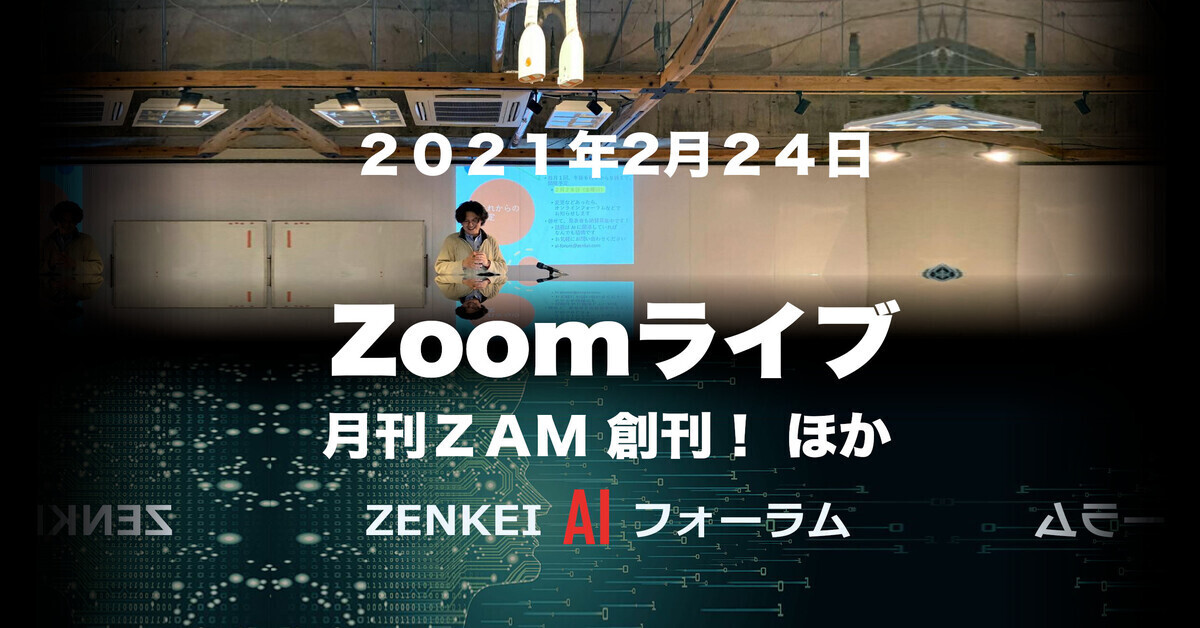
\includegraphics[width=1.5\textwidth,height=0.6\textwidth]
        {images/ZENKEI_AI_FORUM_zoom_20210224-1200x628_fb.jpg}
    };  
  \end{tikzpicture}\\
  \bfseries \Huge \color{white} 第 \thechapter 章 \color{black}\\
} % label
{0pt} % spacing
{} % in front of the title
[]

\chapter{当日のイベントの模様}
\label{sec:introduction}

\begin{tikzpicture}[remember picture, overlay]
  \node[xshift=-2.05cm,yshift=-2.93cm] at (current page.north east){
    \textcolor{white}{\bfseries \thepage}
  };  
\end{tikzpicture}

久しぶりの(?)いちきの独演会になりました。
いろんな人の幅広い話題を期待してたみなさま、すみませんでした。
(いろいろ立て込んでいて、フォーラムの計画やスピーカーの手配など、
計画立案している余裕がありませんでした。)

とは言え、いざ始まってみると
オーディエンスとしてフォーラムのみなさんが参加してくれて、
とてもうれしかったし、イベントとして単調にならなくて助かりました。

\vspace{1cm}

\begin{tikzpicture}
  \node[anchor=center] at (0, 0){
    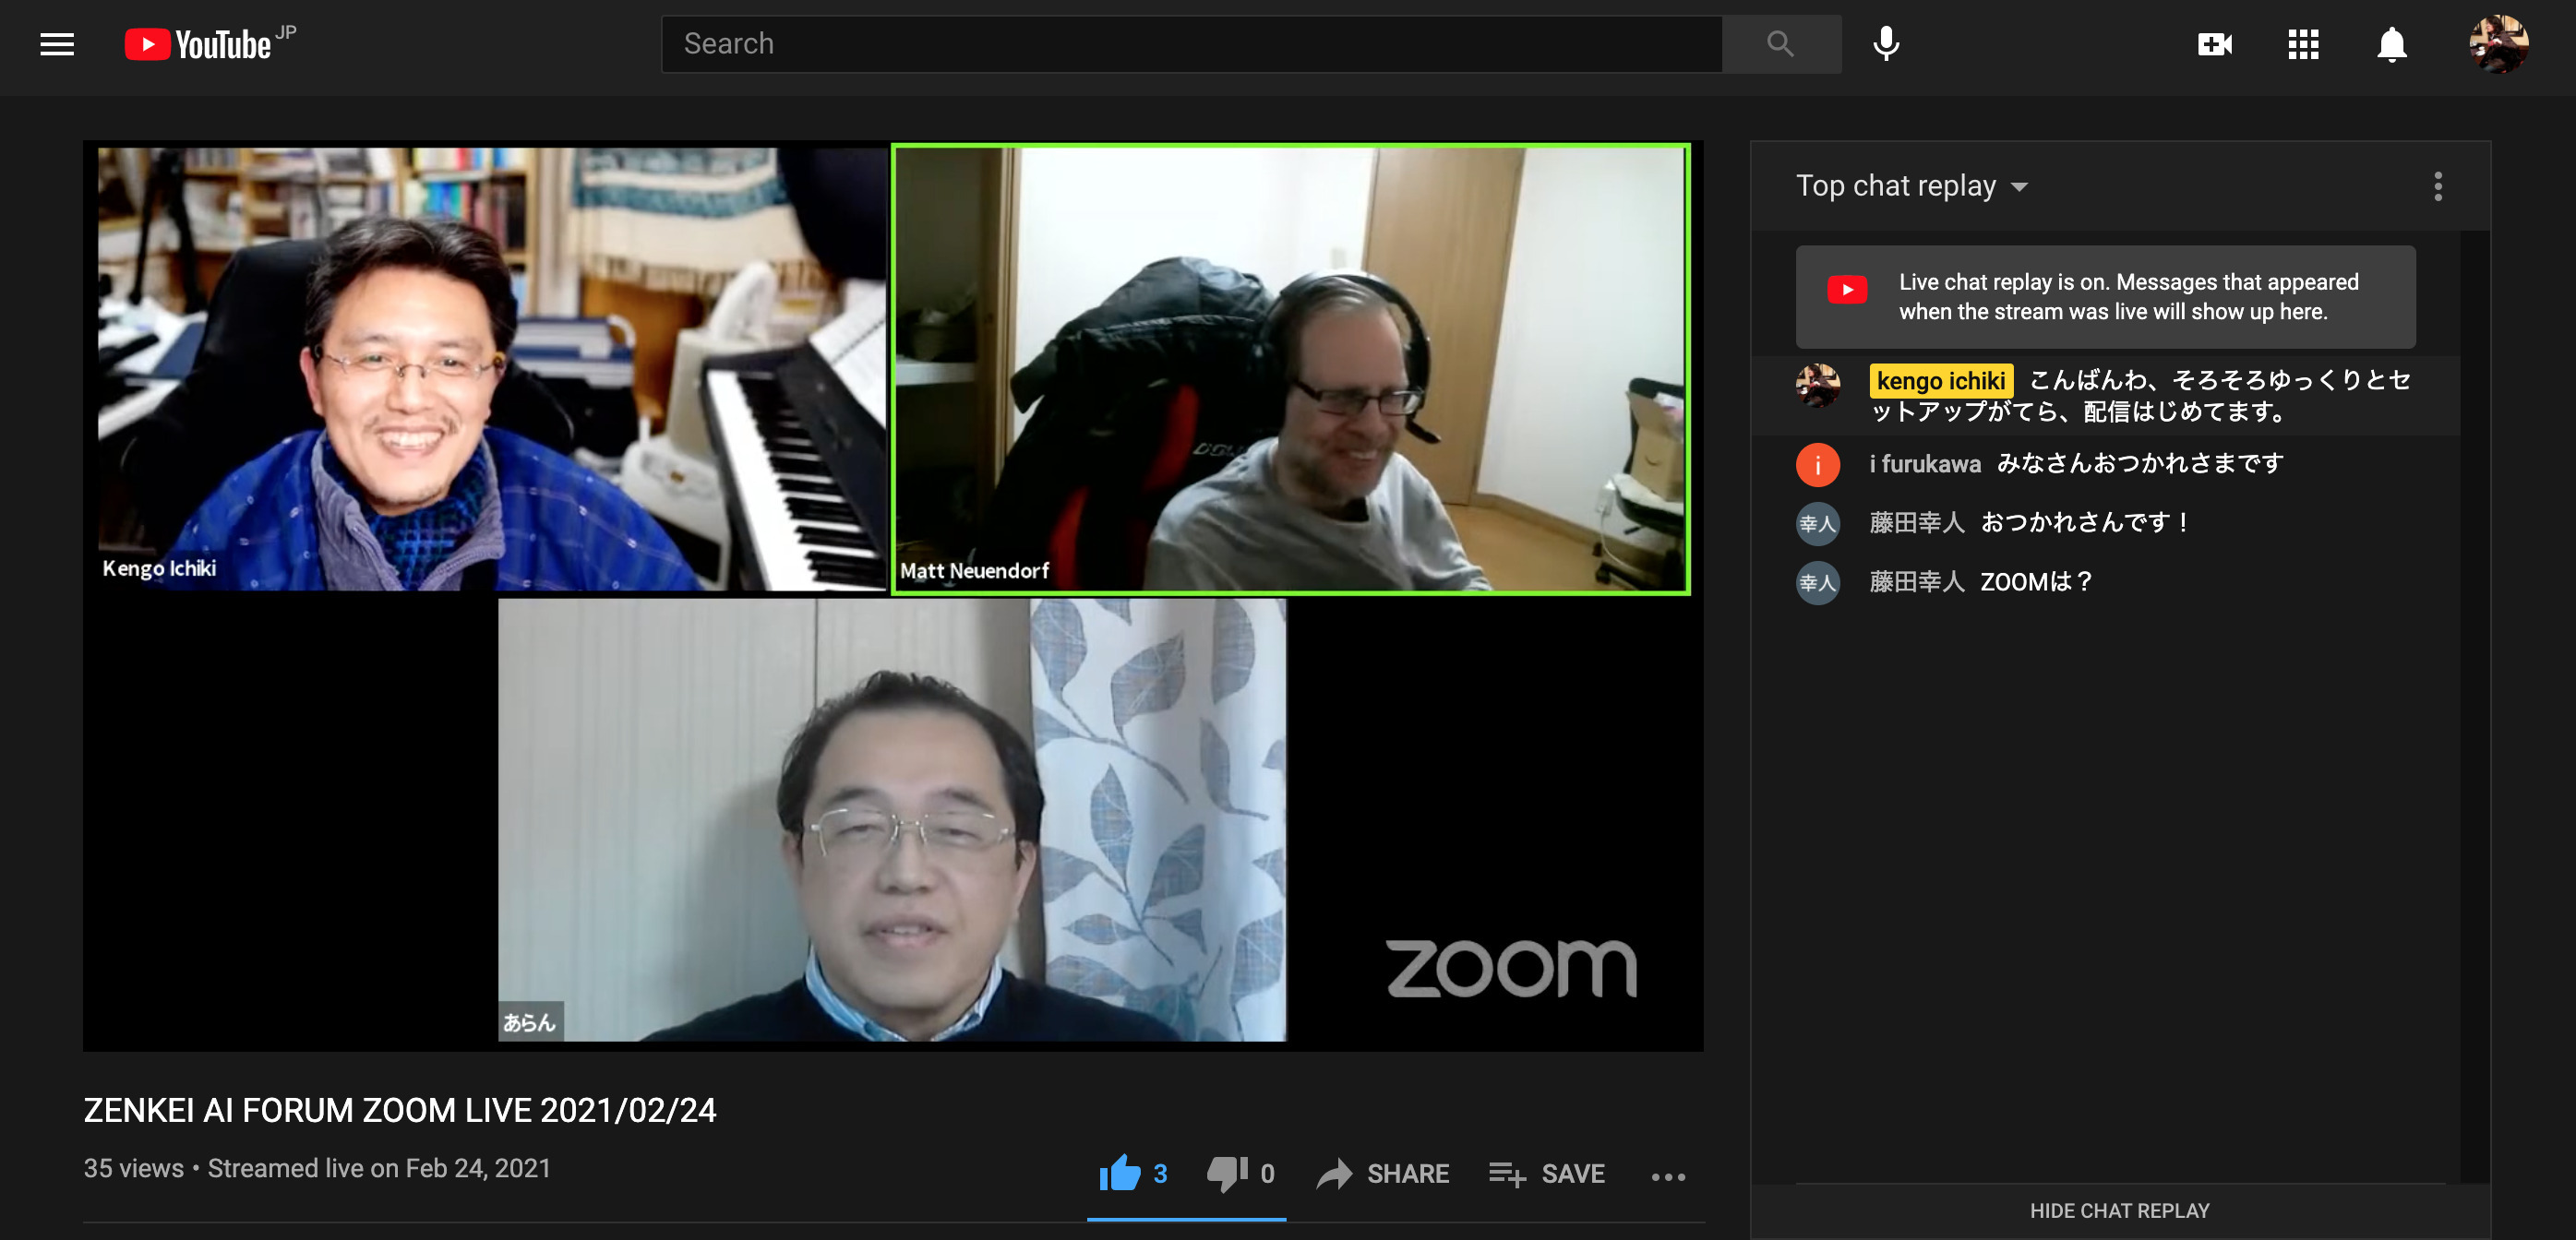
\includegraphics[width=\textwidth]
      {images/youtube.jpg}
  };  
\end{tikzpicture}

ZOOM には Matt さんとあらんさんがきてくれて、
トピックの合間の座談タイムでいつものわたしの無茶振りな質問に
(一部、英語になりましたが)答えてくれました。
また YouTube のチャットには furukawa さんがきてくれて、
コメントいただきました。
みなさん、いつもありがとうございます。


\AddToShipoutPictureBG*{%
  \AtPageLowerLeft{%
    % Your background image here
    \includegraphics[width=\paperwidth,height=\paperheight]%
      {images/ZAM202102-p04-bg.jpg}
  }%
}%
内容は、これから紹介していくように、以下の3つのトピックを話しました。
\begin{itemize}
\item {\gtfamily\bfseries  
  【第 \ref{ch:zenza} 章】 はじめに}\\
  ここ1ヶ月の時事ネタから話題をピックアップ
\item {\gtfamily\bfseries  
  【第 \ref{ch:ai-news} 章】 AI 最近の話題から}\\
  最近画像分類で SOTA を更新したと話題の NFNets を紹介
\item {\gtfamily\bfseries  
  【第 \ref{ch:zam} 章】 『月刊 ZENKEI AI MAGAZINE』創刊}\\
  1月のフォーラムで創刊すると宣言した ZAM を実際に刊行
\end{itemize}

\vspace{1cm}

\begin{center}
\color{teal}
\begin{tikzpicture}
\node[regular polygon, regular polygon sides=7, 
      minimum size=8cm,inner sep=0pt](h)  {}; 
\foreach \i [count=\next from 2] in {1,...,7}
  {% 
   \draw (h.corner \i) to [ornament=81] (h.corner \next);
   \pgfmathtruncatemacro{\next}{mod(\next,7)}%
  }
  \node[inner sep=6pt,yshift=1.5cm] (text) at (h.center){
    \calligra \HUGE Zenkei};
  \node[inner sep=6pt] (text) at (h.center){
    \calligra \Huge AI};
  \node[inner sep=6pt,yshift=-1.5cm] (text) at (h.center){
    \calligra \Huge Magazine};
\end{tikzpicture}
\color{black}
\end{center}

\vspace{2cm}

% 2
\begin{tikzpicture}[remember picture, overlay]
  \begin{scope}[thick,rounded corners=8pt,
      xscale=1.3, xshift=-1.75cm, yshift=-3.5cm] at (current page.south)
  \draw (0, 2) -- (2.5, 2) -- (1.5, 0) -- (3, 0);
  \draw (3, 0) -- (4, 2) -- (5, 0);
  \draw (5, 0) -- (6, 0);
  \draw (6, 0.8) -- (10, 0.8)
    -- (10.7, 2) -- (11.7, 0) -- (12.7, 2) -- (12.7, 0) -- (14, 0);
  \end{scope}
\end{tikzpicture}


\newpage

\chapter{はじめに}
\label{ch:zenza}

\begin{tikzpicture}[remember picture, overlay]
  \node[xshift=-2.05cm,yshift=-2.93cm] at (current page.north east){
    \textcolor{white}{\bfseries \thepage}
  };  
\end{tikzpicture}

発表者が自分だけとは言え、ウォーミングアップは必要だろうということで、
いつも通り「前座」をやりました。
内容は、時事ネタを3つほど取り上げて、しゃべりました。

\begin{multicols}{2}

\section{追悼 Chick Corea}
\begin{tikzpicture}[remember picture, overlay]
  \node[xshift=-4.6cm,yshift=-5.4cm] at (current page.center){
    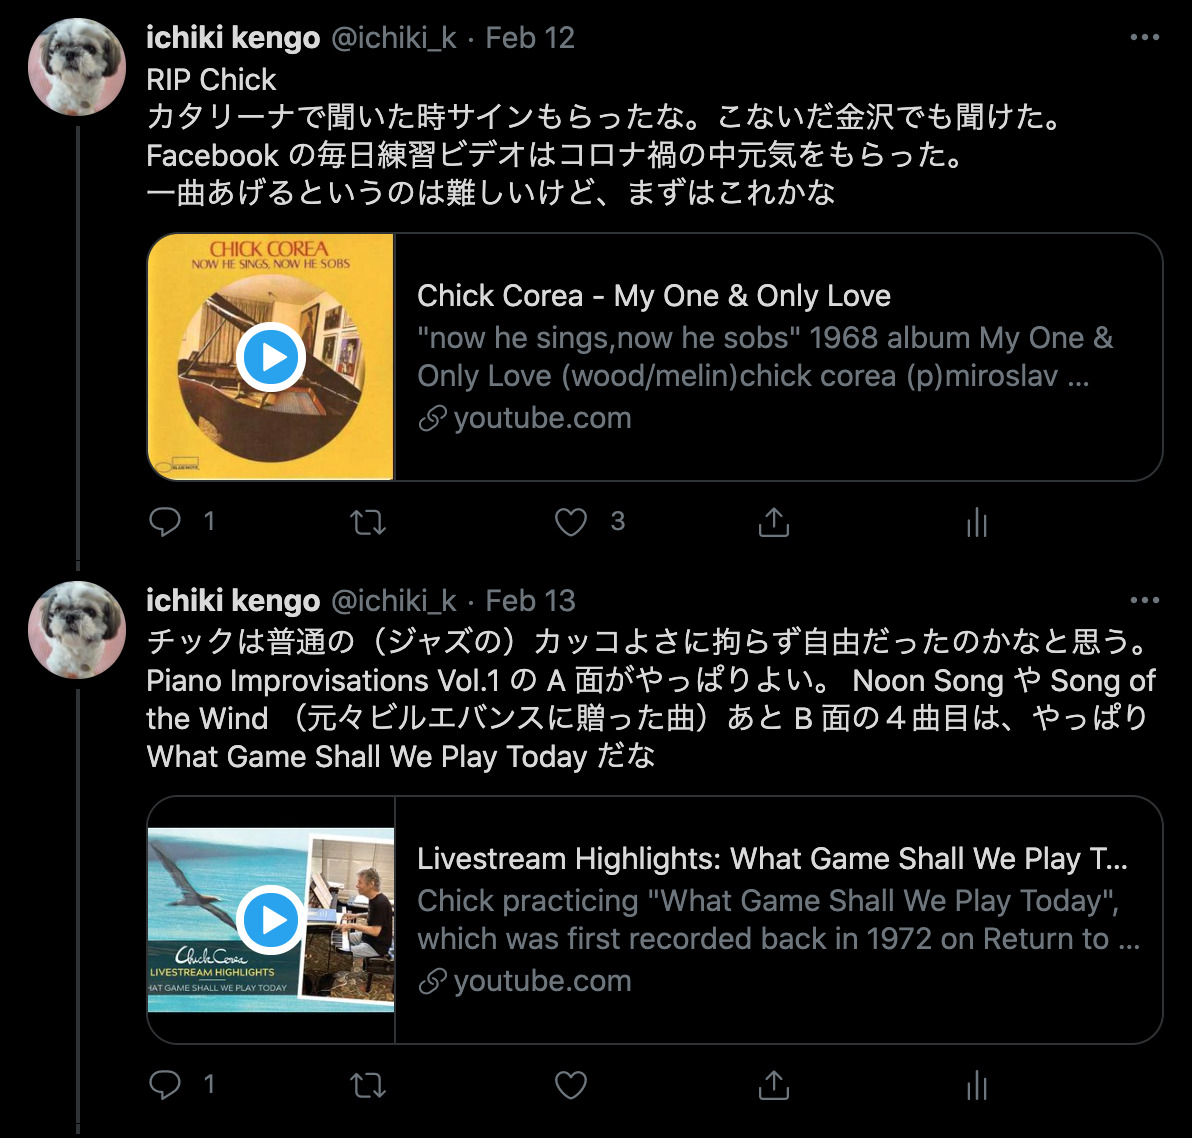
\includegraphics[width=0.63\textwidth]
      {images/chick-01.jpg}
  };  
\end{tikzpicture}

\vspace{7.8cm}

このひと月の間に起こった出来事の中で、個人的に一番大きな出来事は、
Jazz Pianist の Chick Corea 氏が亡くなったというニュースでした。

わたしは家にテレビがないので、日々のニュースなどはインターネットを通じて
目にすることになります。主に Twitter のタイムラインで、
フォローしてる人たちのつぶやきから「あぁ、こんなことが起きてるのか」
と知るのですが、 Chick の訃報も最初だれかミュージシャンの人が
急に古い Chick の曲か写真を(具体的なコメントなしに)ツイートしてて
「まさかね」と思ってあちこち調べたら、フォローしている彼の Facebook
のアカウントに「2月9日、79歳で亡くなった」との投稿がありました。

訃報に接した後、徒然につぶやいたツイート
(\url{https://twitter.com/ichiki_k/status/1360031015377330188})
のスクリーンショットを添えておきます。

わたしはこれまで2度 Chick Corea の演奏を生で見たことがあります。
1度はアメリカの LA 郊外に住んでいた頃(1997年から1999年)、
2度目は数年前金沢に Vigil というバンドで来た時です。

\begin{tikzpicture}[remember picture, overlay]
  \node[xshift=-4.6cm,yshift=3.3cm] at (current page.center){
    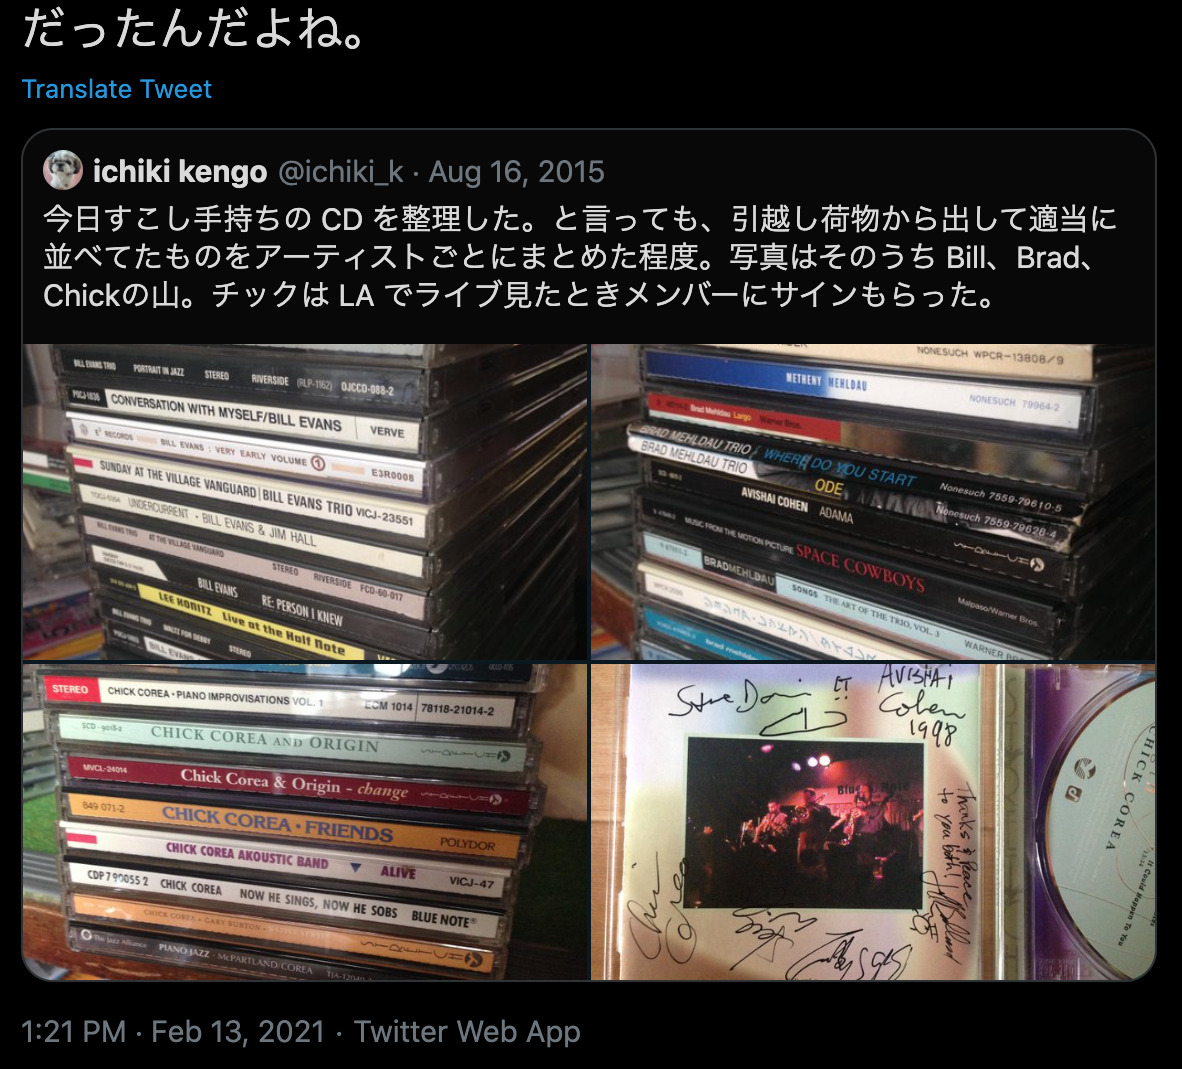
\includegraphics[width=0.63\textwidth]{images/chick-03.jpg}
  };  
\end{tikzpicture}

\vspace{7.9cm}

LA でのライブは当時結成したアコースティックなバンド Origin で、
既に持ってた CD を持って行って、
そこにメンバー全員のサインをもらったのはいい思い出です。
\AddToShipoutPictureBG*{%
  \AtPageLowerLeft{%
    % Your background image here
    \includegraphics[width=\paperwidth,height=\paperheight]%
      {images/ZAM202102-p06-bg.jpg}
  }%
}%

\begin{tikzpicture}[remember picture, overlay]
  \node[xshift=-4.6cm,yshift=-8.3cm] at (current page.center){
    
\includegraphics[width=0.63\textwidth]{images/chick-05.jpg}
  };  
\end{tikzpicture}

\vspace{9cm}

Chick は世間的には Return to Forever でのエレクトリックな側面が有名ですが、
わたしが聴き始めたのはそのブームが終わった辺りからで、
ちょうど ``Akoustic Band'' くらいから(リアルタイムで)聞いてきたことになります。
その後、彼のキャリアを遡ったりもしましたが、
個人的に Piano が好きというのもあって
Pianist としての Chick がわたしにとっての Chick です。
ツイートでも何曲か好きな演奏をピックアップしました。
\begin{itemize}
\item My One and Only Love
\item Song of the Wind
\item Someone to Watch Over Me
\item Yellow Nimbus
\end{itemize}
網羅するのは無理だし、かなり偏った選曲ですが。

\begin{tikzpicture}[remember picture, overlay]
  \node[xshift=4.6cm,yshift=-5.5cm] at (current page.center){
    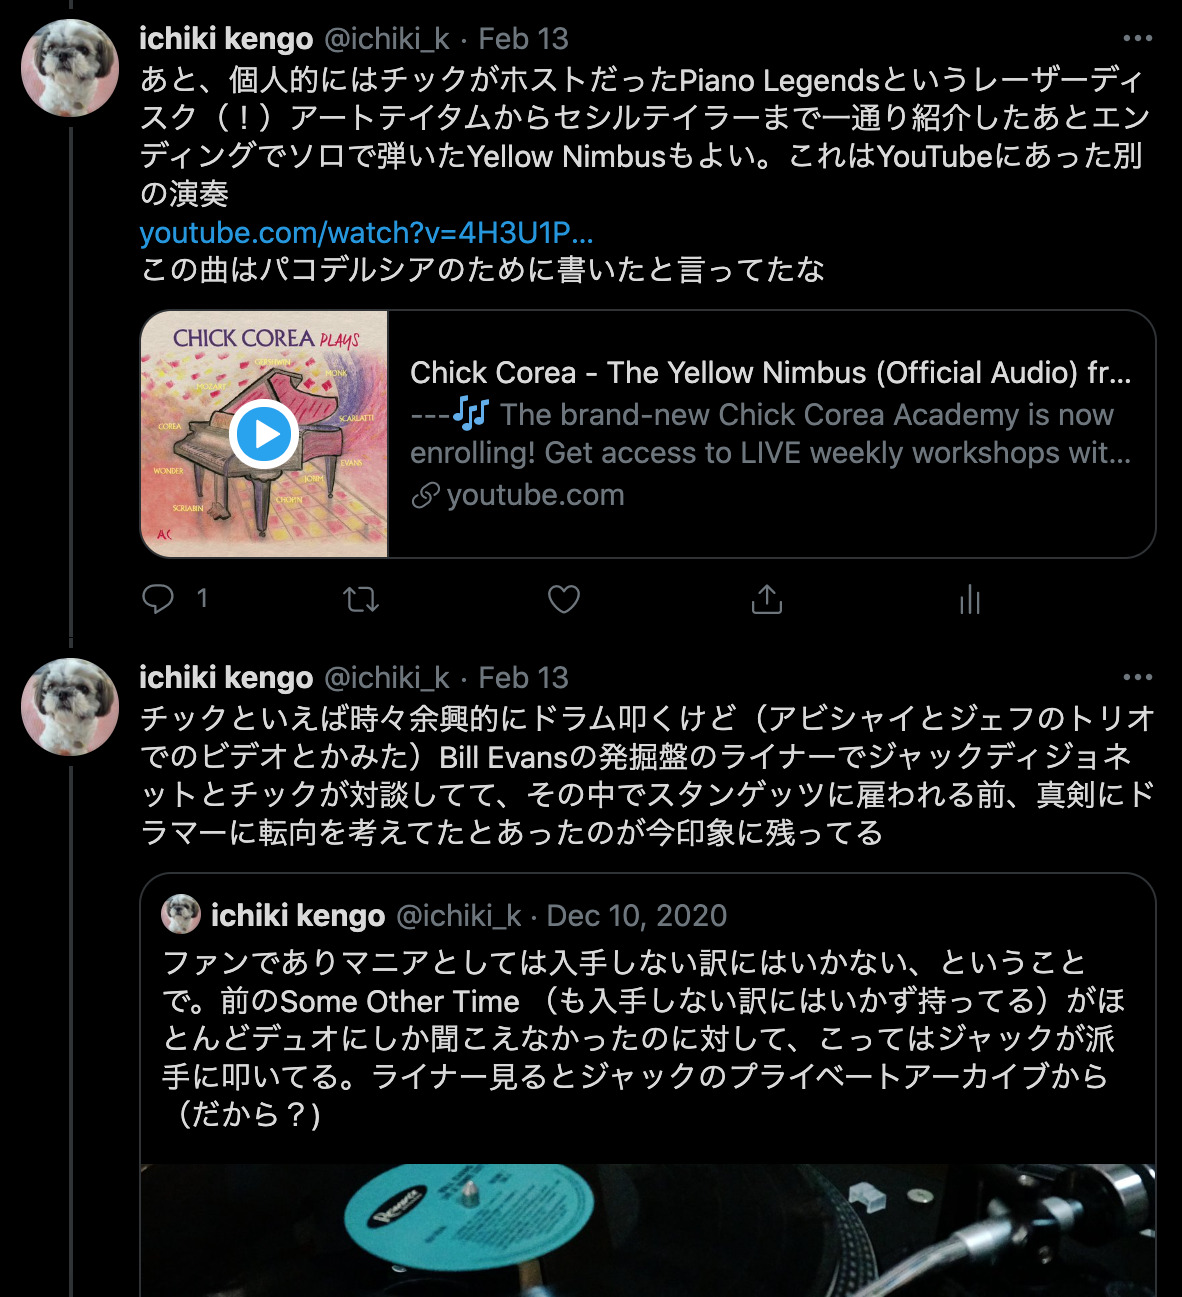
\includegraphics[width=0.63\textwidth]{images/chick-06.jpg}
  };  
\end{tikzpicture}

\vspace{10cm}


実際に去年の春頃のコロナ禍による(自主的)ロックダウンに伴う
環境の変化に際してわたしの気持ちを支えてくれた大きな要素の1つは音楽で、
その中でも Chick が Facebook で毎日配信していた練習ビデオでした
(と実際につぶやいてますね
\url{https://twitter.com/ichiki_k/status/1242301669200674816})。

\begin{tikzpicture}[remember picture, overlay]
  \node[xshift=-4.6cm,yshift=0.0cm] at (current page.center){
    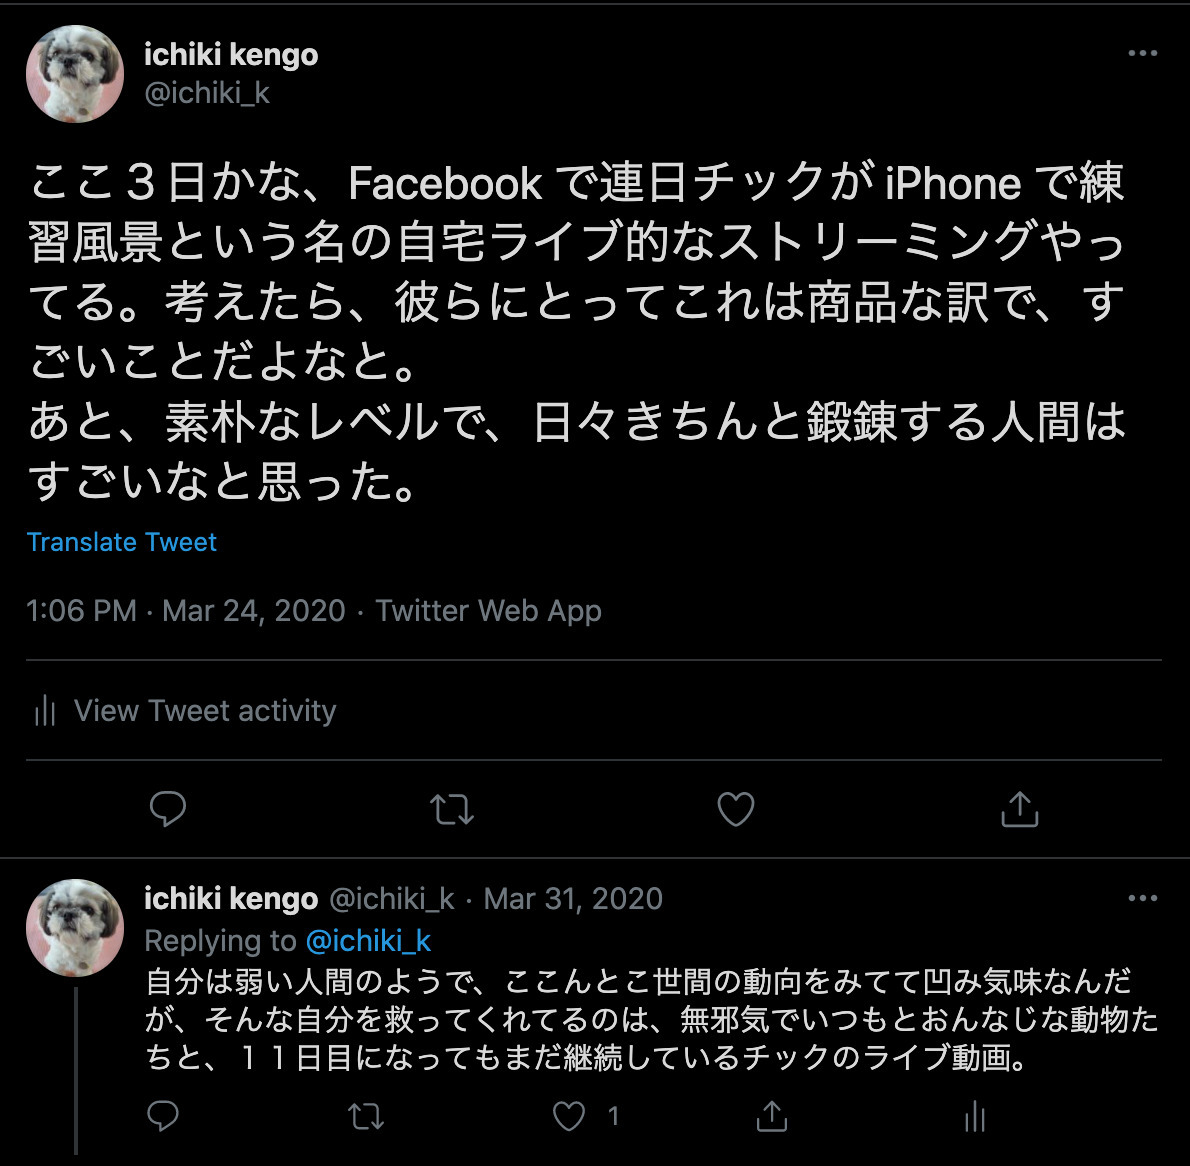
\includegraphics[width=0.63\textwidth]{images/chick-08.jpg}
  };  
\end{tikzpicture}

\vspace{10cm}

これからは YouTube などで Chick の演奏や映像を見るときの気持ちが変わるんだろうな。
ご冥福をお祈りします。 R. I. P.

\vspace{3cm}

\section{「忍耐力」}
\begin{tikzpicture}[remember picture, overlay]
  \node[xshift=4.6cm,yshift=4.8cm] at (current page.center){
    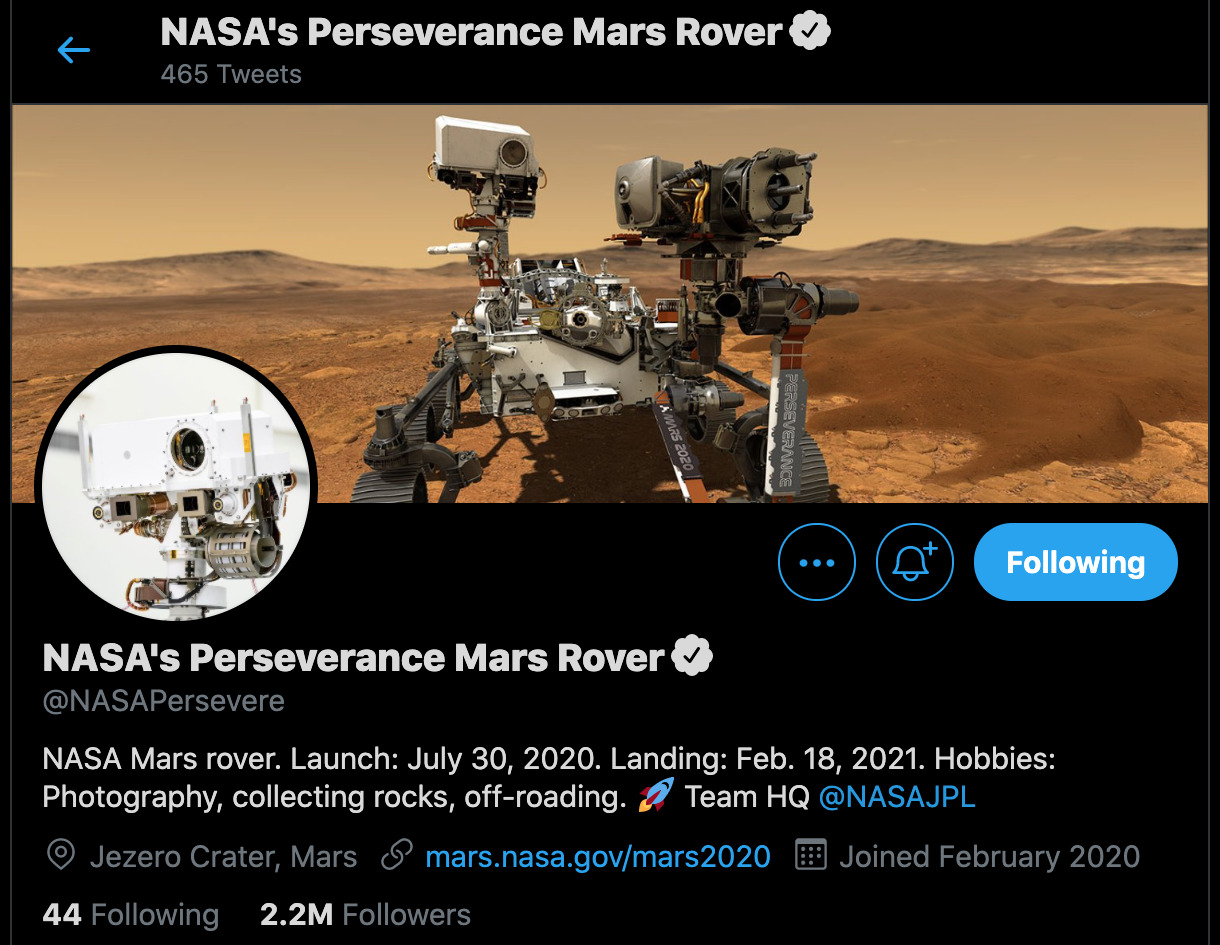
\includegraphics[width=0.63\textwidth]{images/perseverance-01.jpg}
  };  
\end{tikzpicture}

\vspace{6.5cm}

みなさんは英語は得意ですか?
授業や受験でたくさん英単語を覚えましたね?
``perseverance'' という単語は、大学受験で出てきたか
ちょっと記憶が怪しいですが、意味は分かりますか?
分からない人でも今この単語を目にしたりしてると思いますが、
思い当たらないかな?
あ、分かった。それはきっと悪しきカタカナ語のせいですね。
わたしがこの英単語にカタカナを当てるとすると
「パーシ{\bfseries ビ}アランス」ですが、ニュースなどを見ると
「パーサヴィアランス」という表記を使っていますね。
(「{\bfseries 太字}」はアクセントという気持ち。)

と、前振りが長くなりましたが、
このひと月の間に起こった出来事のもう1つの話題は
火星探査機 Perseverance の着陸成功のニュースです。
(公式ツイッターアカウントはこちらです。
\url{https://twitter.com/NASAPersevere})

当日のビデオでもコメントしましたが、
わたしたちは地球の上で日々あくせく暮らしていますが、
人類は宇宙に向かって着実に進んでいるんだなぁ、と感じました。
わたしが大学の頃から大好きだった Star Trek: The Next Generation の
オープニングのナレーションを引用しておきましょう:
\begin{quotation}
  \noindent
  {\it Space: the final frontier}.
  These are the voyages of the starship Enterprise.
  Its continuing mission: to explore strange new worlds.
  To seek out new life and new civilizations.
  {\it To boldly go where no one has gone before!}
\end{quotation}


\AddToShipoutPictureBG*{%
  \AtPageLowerLeft{%
    % Your background image here
    \includegraphics[width=\paperwidth,height=\paperheight]%
      {images/ZAM202102-p08-bg.jpg}
  }%
}%
\subsection{大丸拓郎さん}
今回この火星探査機 Perseverance のことを知ったきっかけの1つに、
現在 NASA JPL で働いている日本人の大丸拓郎さんの Twitter の一連の投稿がありました。
しばらくは「へぇ、日本の人が NASA でバリバリやってるんだな、すごいな」と
普通に感心してたんですが、今回の盛り上がりに際して大丸さんの Note の記事
%『\textgt{日本人がNASAで働くには}』
『{\gtfamily\bfseries 日本人がNASAで働くには}』
(\url{https://note.com/takurodaimaru/n/n17e74fc49339})
を読みました。そして、いろんな意味ですごい人だなとの思いを深くしました。


この記事は大丸さんが現在の職場 (JPL) に至るまでの人生を振り返ったものです。
そういう形でまとめた故なのか、
彼自身がきちんと計画し、行動し、達成するタイプの人なのか
(おそらく、その両方なんでしょう)
本当に1つの目標(JPL で働くこと)に向かって
継続的に着実に\ruby{歩}{あゆ}みを進めて行ったんだなぁ、と。
これを読んで、有名な Steve Jobs の Stanford 大学の
2005 年の卒業式でのスピーチで喋った
``connecting the dots'' の話のことを思い出しました。
そこで彼は、
\begin{quotation}
  \noindent
  人生において、
  点と点の間に線がつながっているのは、
  その時には分からないけれど、
  事後的に、あとで振り返った時には、明瞭に見えるものだ
\end{quotation}
(意訳)とも語っていました。
わたしが感じたのは、
「今」にいる自分はとにかく「今」に全力を注ぐのが正しいのだろう、
その積み重ねをあとで振り返ると、そこに意味や結果が見えてくるのだろう、と。
    

あと今回きちんと大丸拓郎さんの記事を読んで、
自分とダブるところがいくつかあって、勝手に親近感がアップしました。
1つは大学が同じ(トンペイこと東北大学)ということ。
あと1つは JPL (これは最初から、そうだなと思ってたことですが)。
知らない人は知らないことですが、
歴史的な経緯があって NASA の JPL ことジェット推進研究所というのは
カリフォルニアにあって、それは元々ここが Caltech の研究所だったからのようです。
「Pasadena 懐かしい」という、これも一方的な親近感アップポイント。


と同時に、彼とわたしの違いもひしひしと感じました。
わたしは人生を振り返ると、結構、無自覚に生きてきたなと思います。
恐らくゴール指向で生きてないということなのかな。
一方、大丸さんは明確な目的意識を持って、
きちんと戦略的に計画をたてて、
きちんと行動してきたんだな、と。
こう言う部分で人生に「差」が付くんですよ、と若者のみなさんにアドバイスしたいですね。

% 3
\begin{tikzpicture}[remember picture, overlay]
  \begin{scope}[thick,rounded corners=8pt,
      %xscale=1.3, yscale=0.7, xshift=-7.5cm, yshift=-6.1cm]
      xscale=1.3, yscale=0.7, xshift=-7.5cm, yshift=-6.8cm]
  \draw (0, 2) -- (3.5, 2) -- (2.5, 0) -- (4, 0);
  \draw (4, 0) -- (5, 2) -- (6, 0);
  \draw (6, 0) -- (7, 0);
  \draw (5, 0.8) -- (9, 0.8)
    -- (9.7, 2) -- (10.7, 0) -- (11.7, 2) -- (11.7, 0) -- (14, 0);
  \end{scope}
\end{tikzpicture}

大丸さんの Note にもいくつかエピソードとして出てきますが、
人生のいろんなことを決定する要素は結局「人」だと思いました。
その時大切になるもの、つまり相手を動かす重要な要素は、
こちらの「熱量」だと。
複数形の ``we'' ではなく単数形の ``I'' できちんと立って勝負する姿勢だと。
その上で成立する「人と人のつながり」こそが大切だと(自分の人生を振り返って)感じた、
という話は拙著『厳密な計算』にも書きました。
こういう認識を確認できたことが、この本を書いたいちばんの収穫でしたね
(我田引水)。

 % 全角スペース

\begin{tikzpicture}[remember picture, overlay]
  \node[xshift=-4.6cm,yshift=-4.0cm] at (current page.center){
    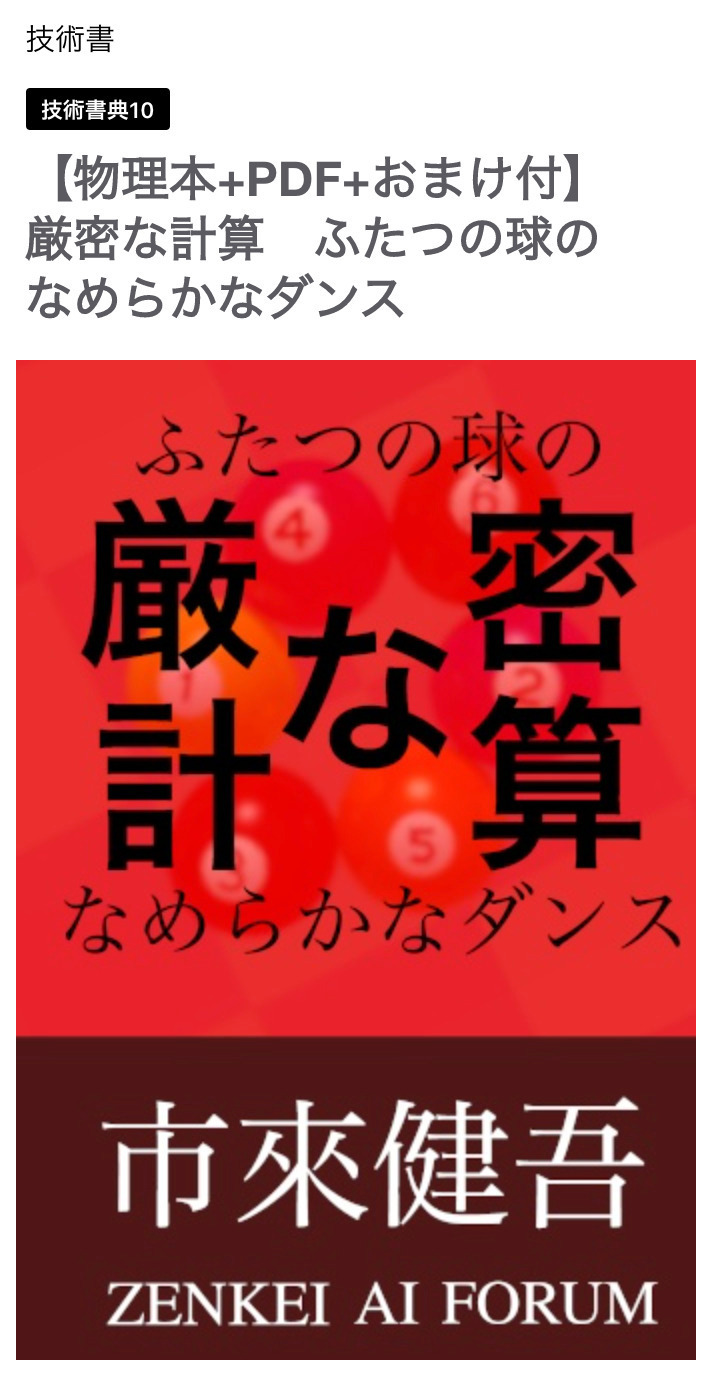
\includegraphics[width=0.63\textwidth]{images/exact-computation.jpg}
  };  
\end{tikzpicture}

\vspace{15cm}

\section{今日の数理ネタ}
\AddToShipoutPictureBG*{%
  \AtPageLowerLeft{%
    % Your background image here
    \includegraphics[width=\paperwidth,height=\paperheight]%
      {images/ZAM202102-p09-bg.jpg}
  }%
}%
『数理クイズ』の、これまでのまとめ(つまり回答編)を「やります!」
と言い続けて数か月がたちますが、すみません。
今月もバタバタしていて準備ができていません。
ということで、今日もお話だけです。
それでも面白い話があったので紹介します。
以下のツイート
(\url{https://twitter.com/potetoichiro/status/1360811105442926592})
です。
\begin{quotation}
  \noindent
  【吃驚仰天!正七角形!?】\\
  なな、なんと、円と2本の放物線の交点を結んで正七角形をつくることができるそうです。先ほど初めて知りわたしもやってみました。そして、その美しさに感動しました。松田康雄先生が発見し、2019年に算額が高見神社に奉納されたとのことです。いつか実物を見に行きたいです!
\end{quotation}
正多角形ですから、円周上に載ることは自明ですが、
同時に2本の放物線の上に載る、
つまりそれらの交点として決まる、と。
美しい。

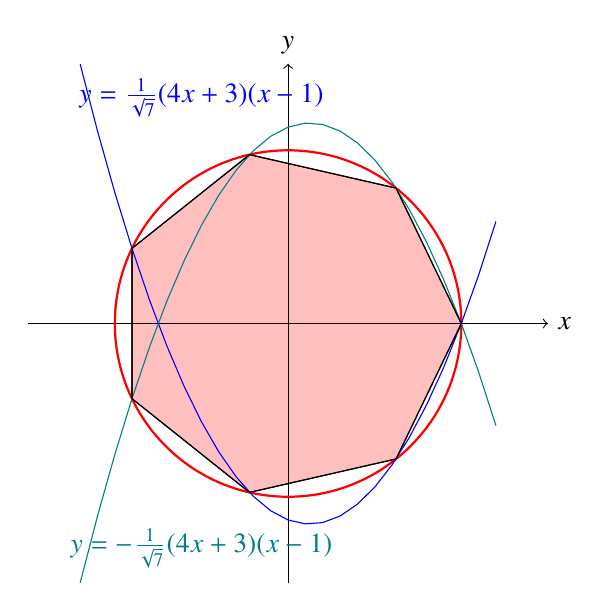
\begin{tikzpicture}[domain=-1.2:1.2,scale=2.2]
\filldraw[fill=pink,domain=0:360,samples=8] plot({cos(\x)}, {sin(\x)});
\draw[->] (-1.5,0) -- (1.5,0) node[right] {$x$};
\draw[->] (0,-1.5) -- (0,1.5) node[above] {$y$};
\draw [red, thick] (0,0) circle (1);
\draw[color=blue] plot (\x,{(4*\x*\x-\x-3)/sqrt(7)}) node[at={(-0.5,1.3)}] {$y = \frac{1}{\sqrt{7}}(4x+3)(x-1)$};
\draw[color=teal] plot (\x,{-(4*\x*\x-\x-3)/sqrt(7)}) node[at={(-0.5,-1.3)}] {$y = -\frac{1}{\sqrt{7}}(4x+3)(x-1)$};
\draw[color=black,domain=0:360,samples=8] plot({cos(\x)}, {sin(\x)});
\end{tikzpicture}


\end{multicols}


\chapter{AI 最近の話題から}
\label{ch:ai-news}
\AddToShipoutPictureBG*{%
  \AtPageLowerLeft{%
    % Your background image here
    \includegraphics[width=\paperwidth,height=\paperheight]%
      {images/ZAM202102-p10-bg.jpg}
  }%
}%

\begin{tikzpicture}[remember picture, overlay]
  %\node[xshift=-2.05cm,yshift=-2.93cm] at (current page.north east){
  \node[xshift=2.12cm,yshift=-2.93cm] at (current page.north west){
    \textcolor{white}{\bfseries \thepage}
  };  
\end{tikzpicture}

みなさん、画像分類、好きですよね?
今日は最近 DeepMind から出た論文で、
画像分類の SOTA となった NFNets を、
サクッと紹介して、ドヤっってしたかった
(けど、オヤっとなった)という話です。


\begin{multicols}{2}

\section{はじめに}
日常的なニュースも、技術的なはなしも、 Deep Learning に関する最新の話題も、
最近わたし Twitter のタイムラインに依存してしまってます
(フィルター・バブルにはまっていることをきちんと自覚して、
その上でツールとして利用できる部分は利用していこうと思ってます。
ミイラにならないように)。
今回の NFNets の件も最初は Twitter でした。
Kaggle の強い人、という認識のある \href{https://twitter.com/ZFPhalanx}{phalanx} さん
のツイート (\url{https://twitter.com/ZFPhalanx/status/1363622203917443072})
\begin{quotation}
  \noindent
  nfnet、過去コンペで試してるけど\\
  毎回こんな感じで結構ヤバイ。
\end{quotation}
です。論文に載ってる結果ではなく自分で計算したらしい図をみると、
「SOTA 更新!」というニュースによくある
「コストがちょっとかかるけど精度は少し上だね」というレベルではなく、
同程度の精度を得るのに必要な epoch 数が既存の40〜50に対して10と圧倒的に速い。

それでちょっと真面目になってググって、論文を見つけました。
``\textbf{High-Performance Large-Scale Image Recognition Without Normalization}''
(\href{https://arxiv.org/abs/2102.06171}{arxiv: 2102.06171})
です。
PDF をダウンロードして著者
(Andrew Brock, Soham De, Samuel L. Smith, Karen Simonyan)
の所属を見て、ちょっとびっくりしました。あの AlphaGO で有名な DeepMind でした。
「画像分類の論文なんて出すんだ」と思いました。
今時の論文は1ページ目に一番大事な図を載せるんですね。
ということで(本文はまだほとんど読んでない段階で)
その目玉の図1をみると、確かに画像分類で SOTA を達成したらしい。
これまでの SOTA だったモデルが比較としてあれこれ出ています。例えば
{\bfseries EfficientNet}。これはしばらくすごいすごいと言われていて、
実際にわたしも使ったことありました
(cf. github: \href{https://github.com/lukemelas/EfficientNet-PyTorch}{lukemelas/EfficientNet-PyTorch})。
{\bfseries LambdaNet} というのも最近話題にのぼっていましたが、
こちらはまだきちんと勉強できてません。
これらのモデルに対して精度と学習時間をプロットした図が示されていますが、
精度は高く、学習時間も短く、しかも他のモデルはかすりもしない。
先の \href{https://twitter.com/ZFPhalanx}{phalanx} さんが
論文とは別のデータセットで同様な結果を示していたことと、
著者が DeepMind ということで、
よくありがちな、いい結果だけをピックアップした、
という訳ではなさそうという印象で、期待が膨らみます。


今回は ZAF の『最近の話題から』ネタとして紹介するつもりだったので、
手早く使えるソースコードを探しました。
DeepMind 自身も GitHub でソースコードを公開してましたが、
TensorFlow ベースで、かつ JAX を使ってるようで
(詳しくないので)パス。
PyTorch での実装がないかと調べたら、以下の2つのコードがヒットしました。
\begin{itemize}
\item github: \href{https://github.com/vballoli/nfnets-pytorch}{vballoli/nfnets-pytorch}
\item github: \href{https://github.com/rwightman/pytorch-image-models}{rwightman/pytorch-image-models}
  の中の \href{https://github.com/rwightman/pytorch-image-models/blob/master/timm/models/nfnet.py}{nfnet.py}
\end{itemize}

先に進む前に一言、ここまで ``NFNets'' と呼んできましたが、
これはどう言う意味かというと ``Normalizer-Free Networks'' ということです。
ここで言っている normalizer というのは batch normalization layers のことです。


\section{実際に、試してみよう!}
ZENKEI AI FORUM で画像分類といえば
何は無くとも「五郎島」ですね。
ということで先日 ViT や BYOL で試した8階級分類のデータセットを使って、
実際に NFNets の実力をみていきましょう。


\section{vballoli/nfnets-pytorch}
先ほど探して見つけた PyTorch 実装の2つのうち、まず最初に
\href{https://github.com/vballoli/nfnets-pytorch}{vballoli/nfnets-pytorch}
のコードで実験していきましょう。
インストールは \texttt{pip} で簡単にできました。
\begin{quote}
  \texttt{\$ pip install nfnets-pytorch}
\end{quote}
実際に使い方は、
既存のモデルに対して、対応する畳み込み層を置き換える関数
\texttt{replace\_conv()} を適用することで NFNets 化します。

そのモデルを既存の \texttt{zenkei\_ai} のトレーニング関数で学習させてみましたが、
どうもうまく学習してくれません。

\begin{tikzpicture}[remember picture, overlay]
  \node[xshift=4.6cm,yshift=-6.5cm] at (current page.center){
    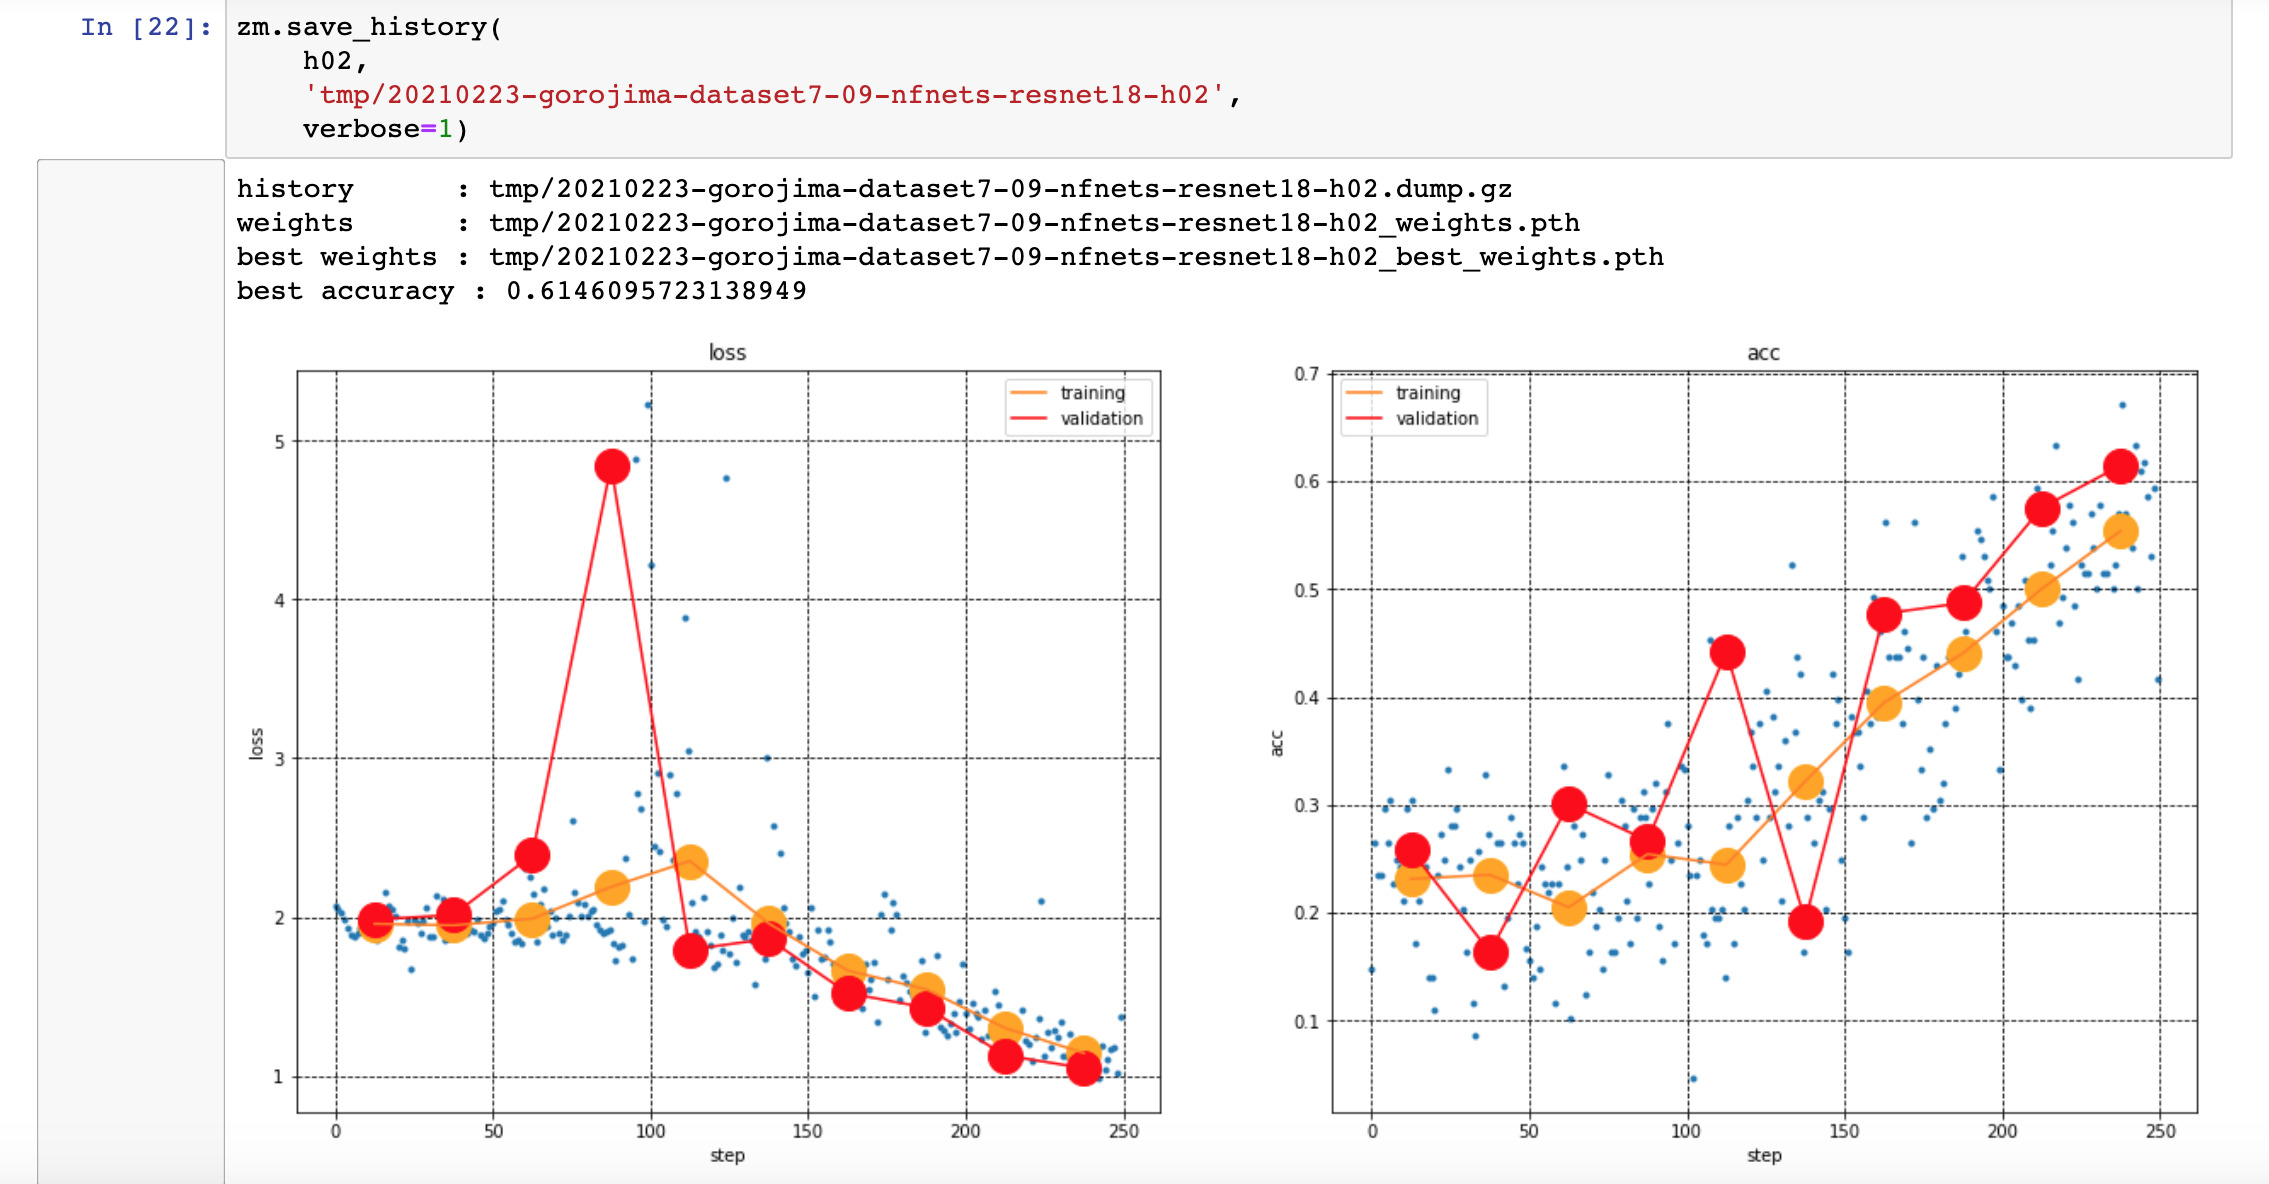
\includegraphics[width=0.63\textwidth]{images/nfnets-vballoli-01.jpg}
  };  
\end{tikzpicture}

\vspace{5cm}

この図を見ると validation accuracy が $60 \%$ を超えていますが、
元々このデータセットは ResNet18 を使うと $10$ エポックもかからないで
$90 \%$ を超えることを考えると、うまくいっていません。


\section{timm - PyTorch Image Models}
次に、たくさんのモデルを含んでいて評判の高い
\texttt{timm} (github: \href{https://github.com/rwightman/pytorch-image-models}{rwightman/pytorch-image-models}) を試してみることにします。
(ちなみに、どうして PyTorch Image Models が \texttt{timm} か、というと
  Py{\bfseries T}orch {\bfseries Im}age {\bfseries M}odels と言うことのようです。難しい。)
\texttt{timm} 自体のインストールは \texttt{pip} でもできますが、
今使いたい NFNets は最新のコミットが必要なので
github から直接 clone してくる必要がありました。
この clone してきたフォルダをパスに追加してモジュールをインポートすると、
\texttt{nf\_resnet26} などの NFNets モデルを使うことができます。

\begin{tikzpicture}[remember picture, overlay]
  \node[xshift=-4.6cm,yshift=-4.5cm] at (current page.center){
    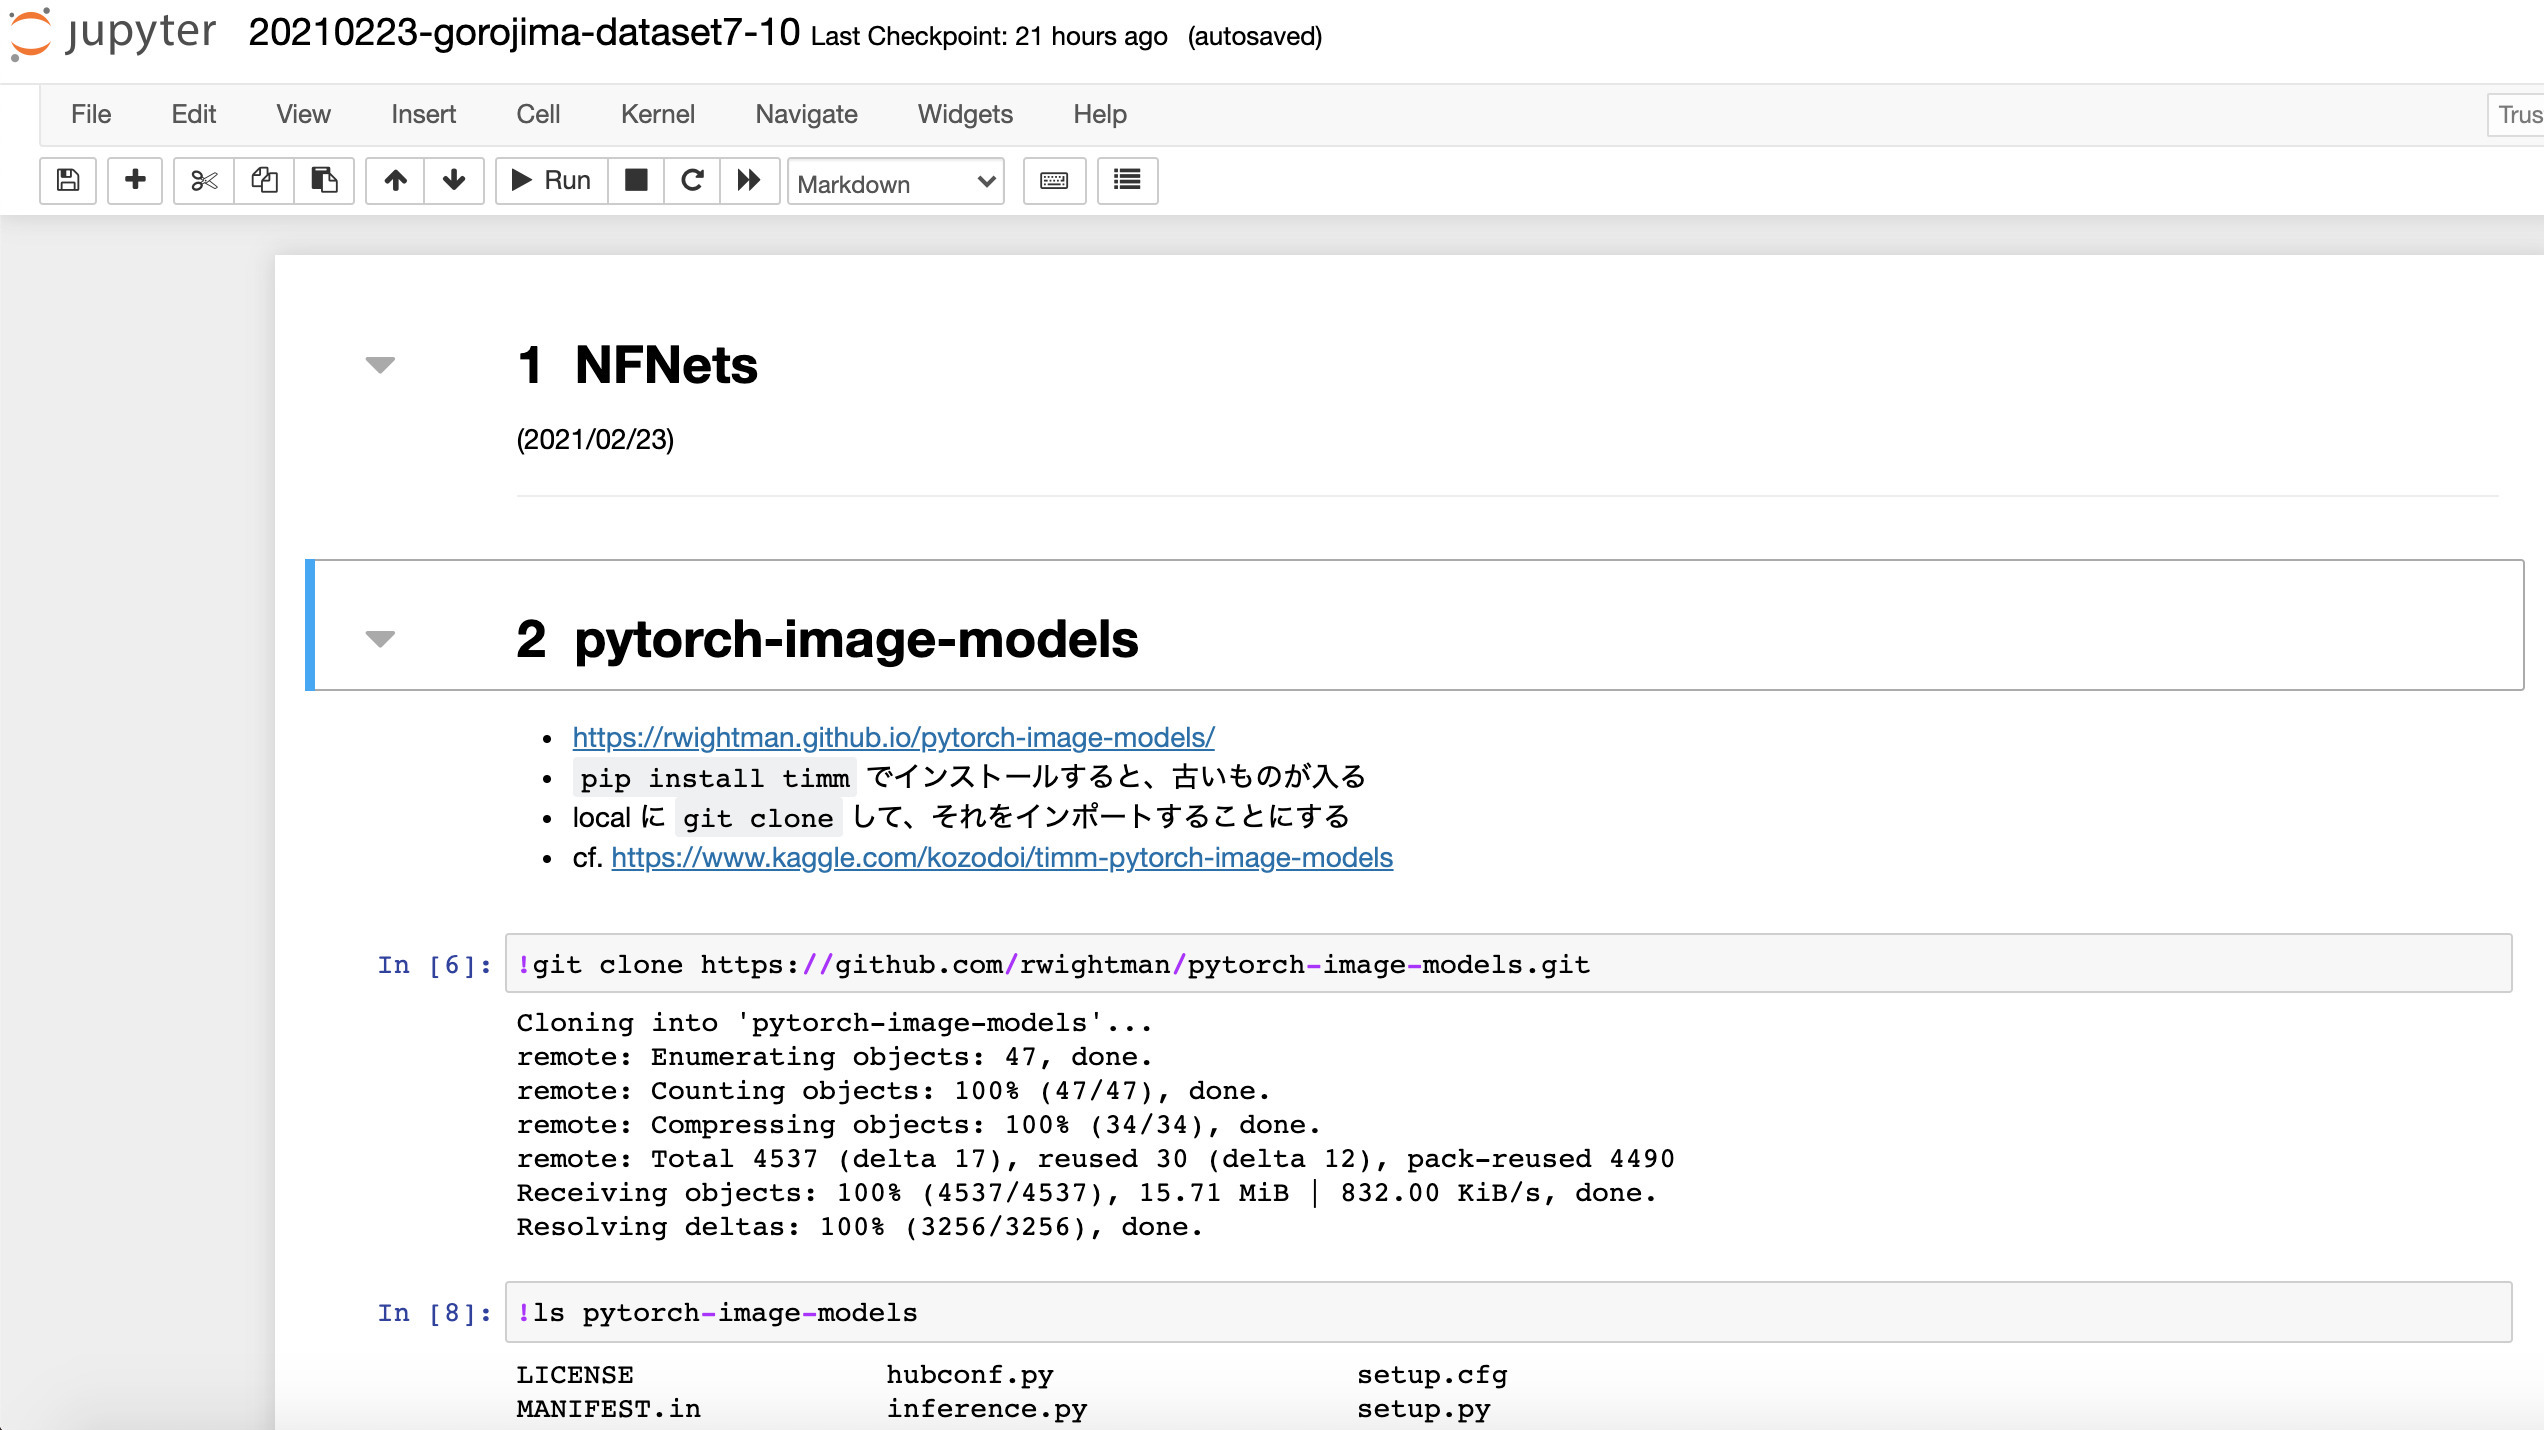
\includegraphics[width=0.63\textwidth]{images/nfnets-timm-01.jpg}
  };  
\end{tikzpicture}

\begin{tikzpicture}[remember picture, overlay]
  \node[xshift=-4.6cm,yshift=-10.0cm] at (current page.center){
    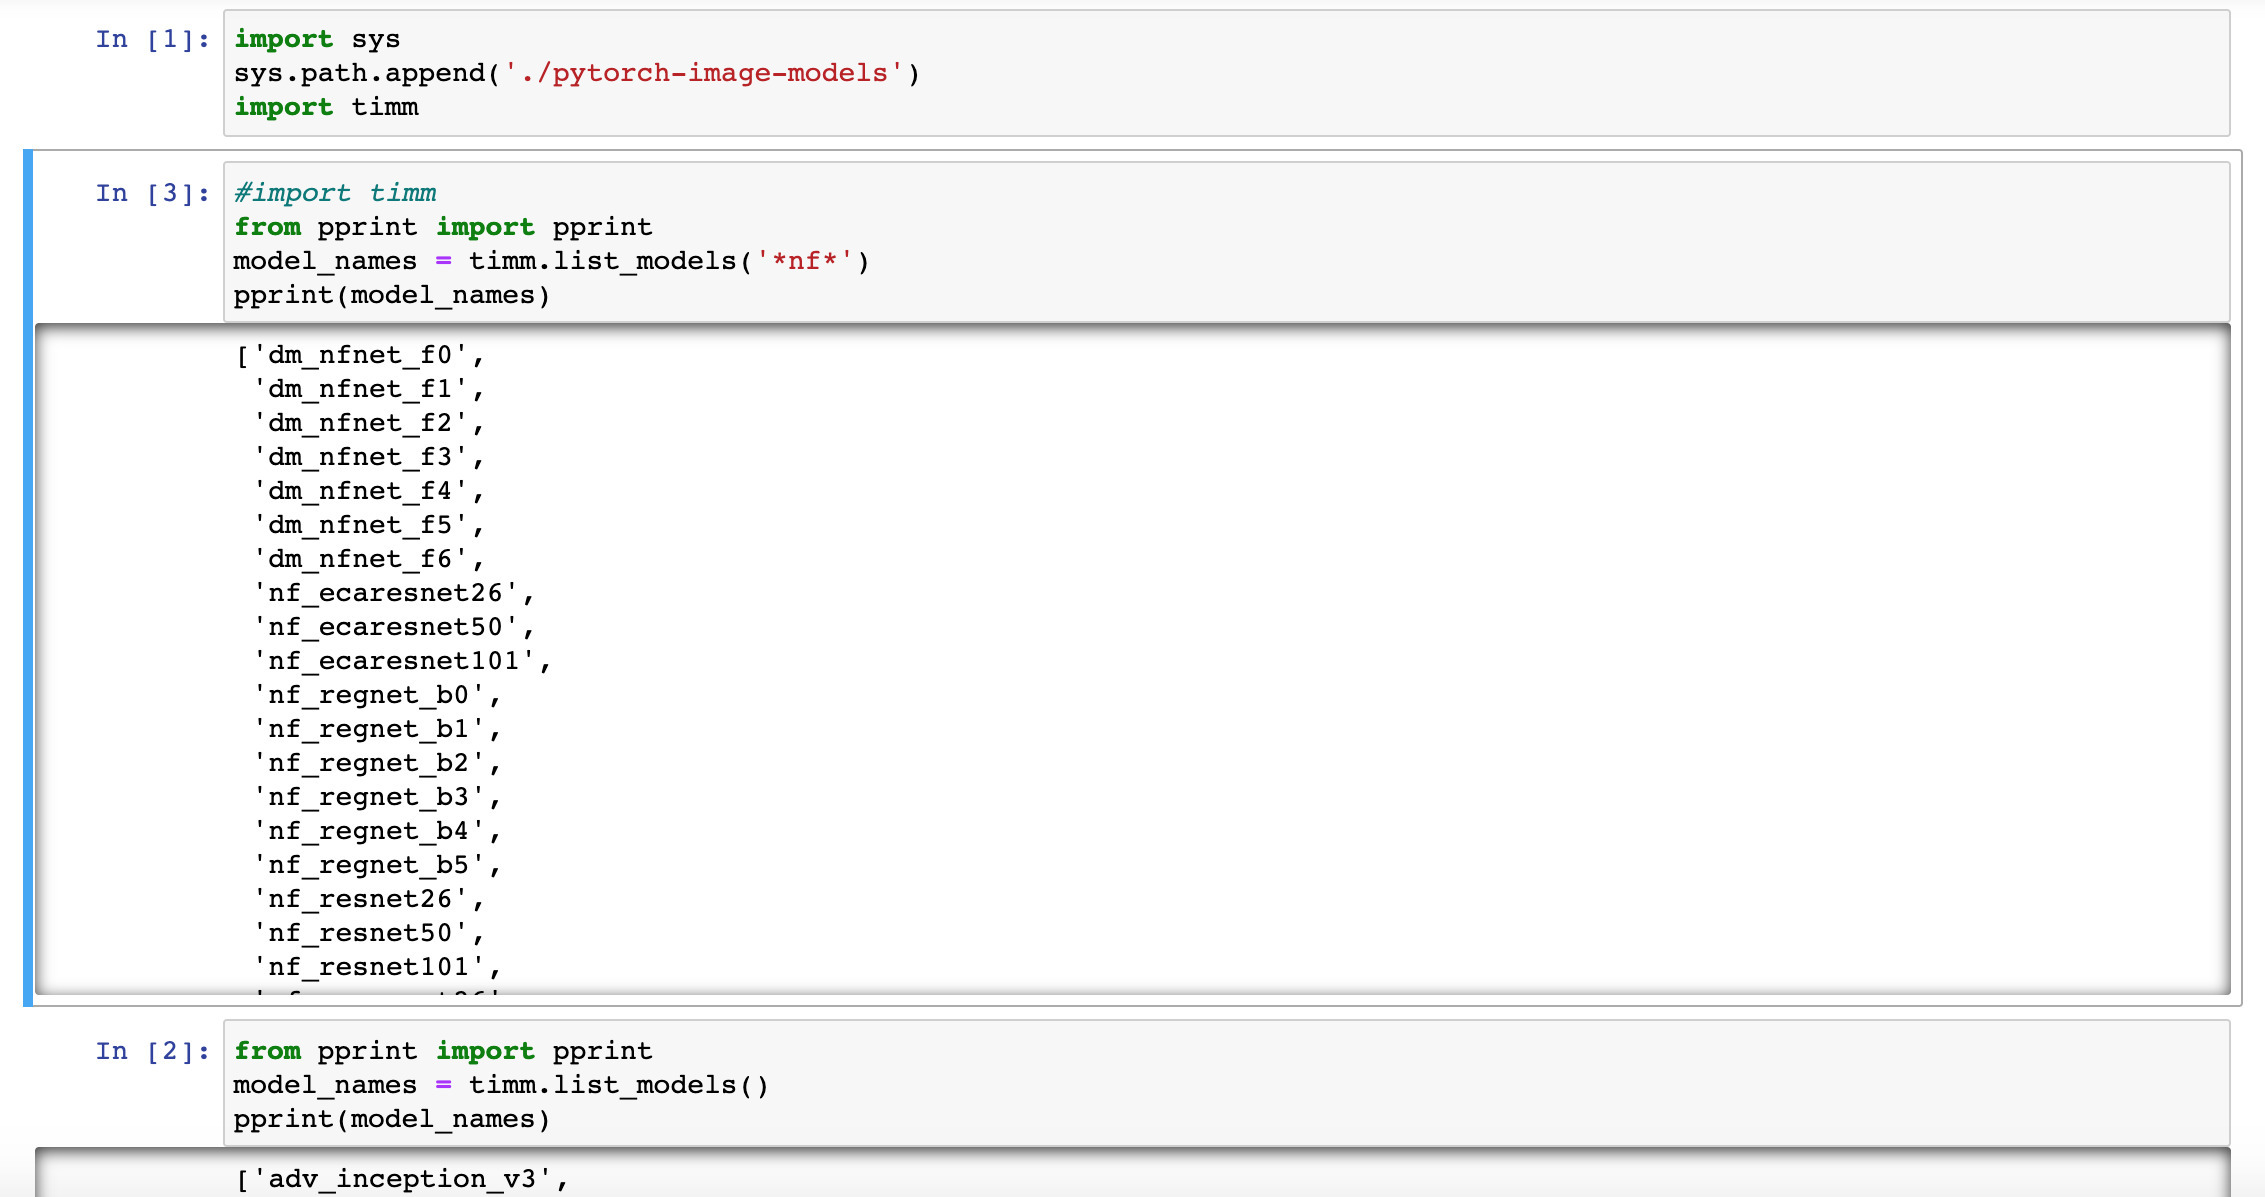
\includegraphics[width=0.63\textwidth]{images/nfnets-timm-02.jpg}
  };  
\end{tikzpicture}

\vspace{8.0cm}
%\vspace{9.0cm}
 %全角スペースで調整……

ここではこの \texttt{nf\_resnet26} を使うことにします。
最初 10 エポック学習させてみると loss は下がり、先の
\href{https://github.com/vballoli/nfnets-pytorch}{vballoli/nfnets-pytorch}
よりは良さそうです。

\begin{tikzpicture}[remember picture, overlay]
  \node[xshift=4.6cm,yshift=4.5cm] at (current page.center){
    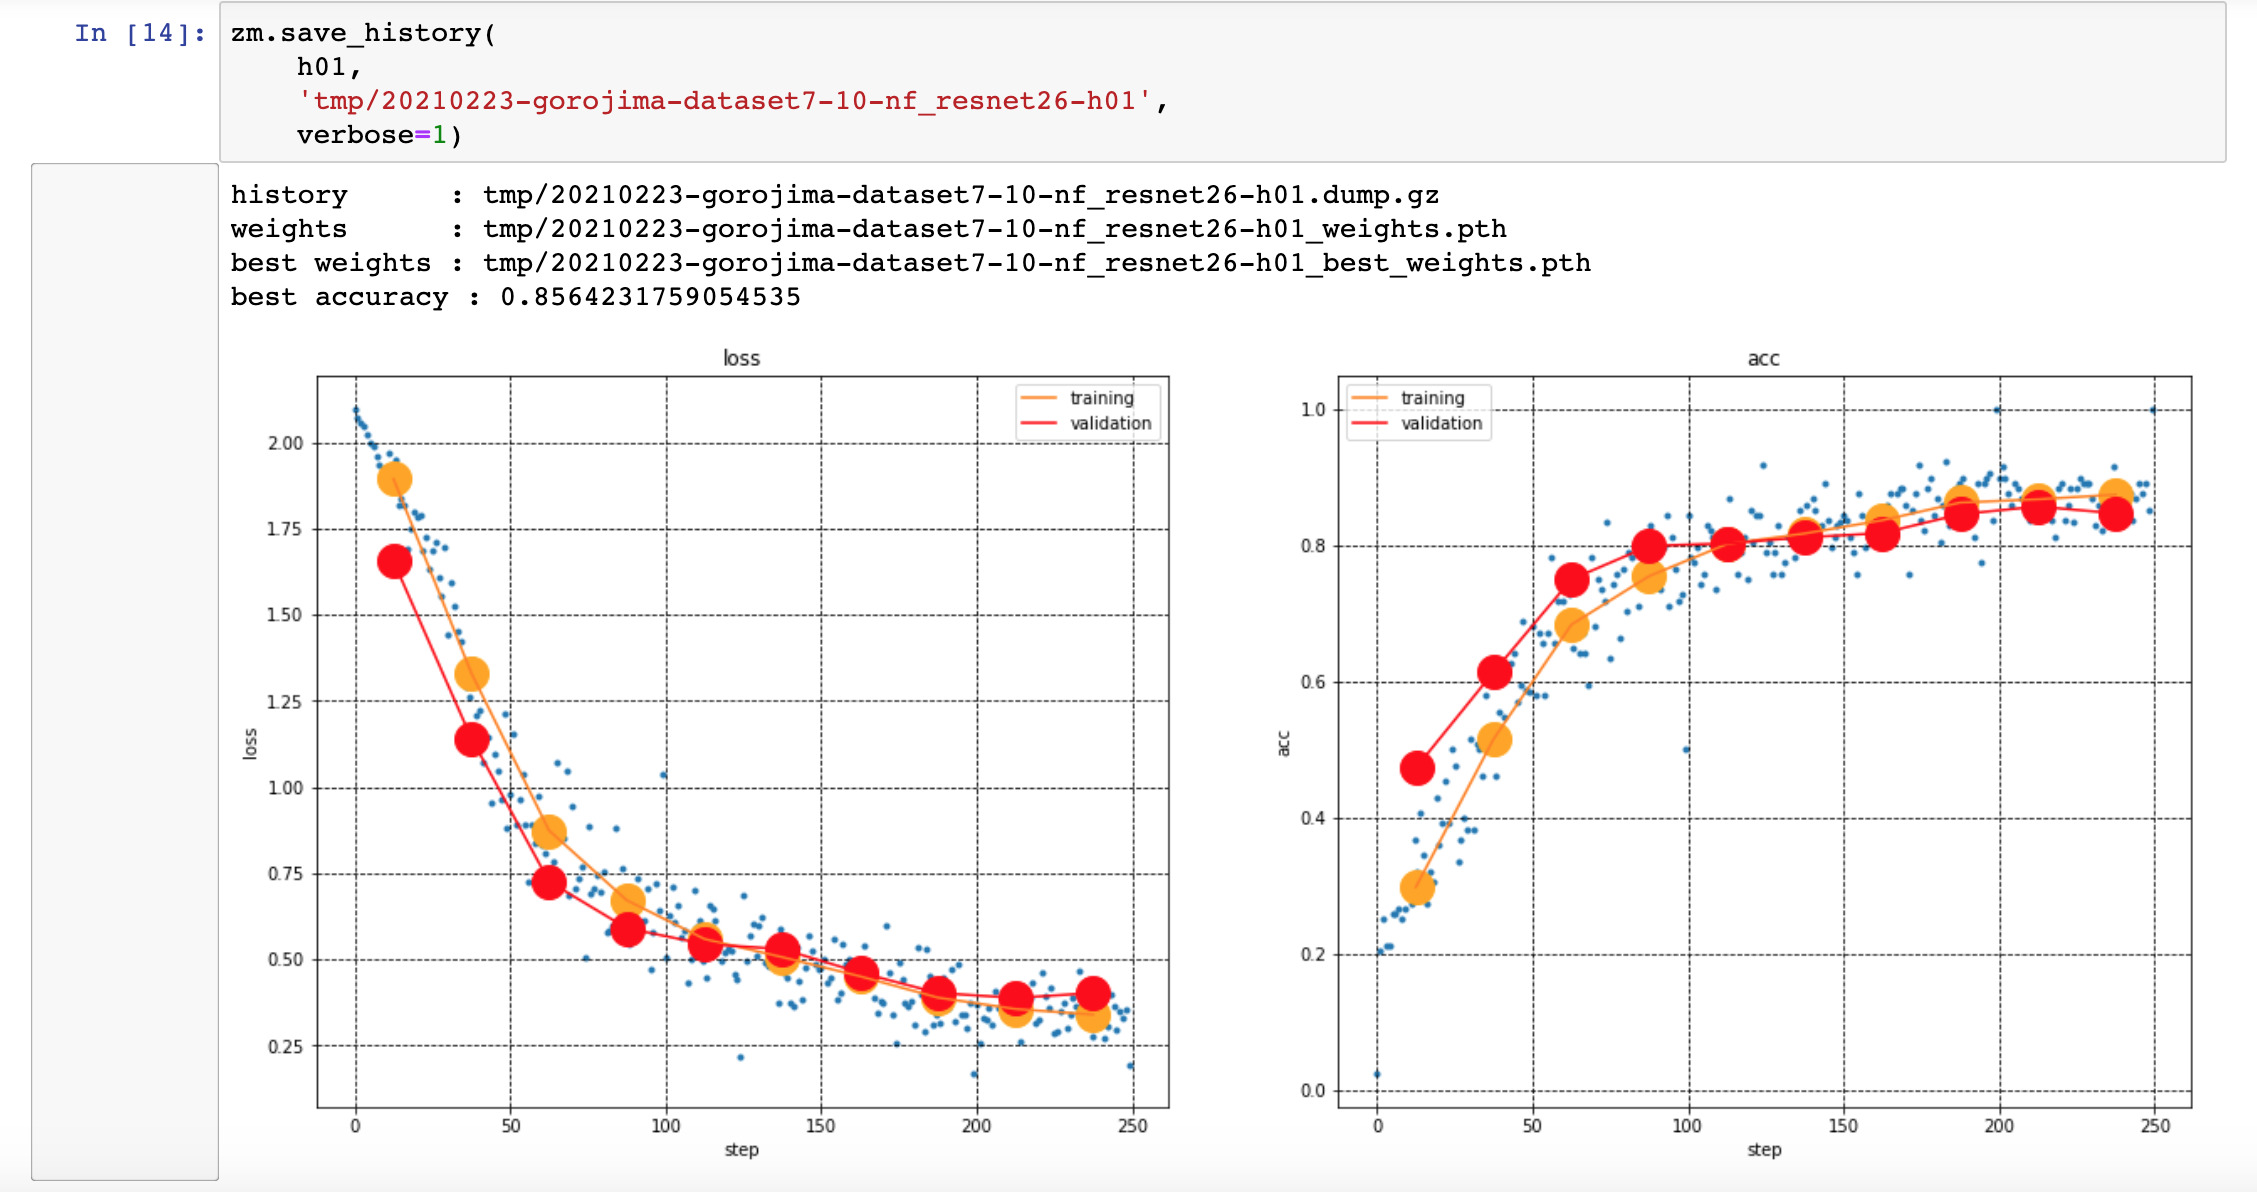
\includegraphics[width=0.63\textwidth]{images/nfnets-timm-03.jpg}
  };  
\end{tikzpicture}

\vspace{4.5cm}

この後も継続して 50 エポックまで学習を続けたところ、
validation accuracy が $91.7\%$ まで上がりました。
この結果だけみるとうまく行ったようにも見えますが、
先にも述べたとおりで、この五郎島データセットを普通の ResNet18 で学習させると
$94\%$ を超えるので、
これでは SOTA を出したモデルとは言えませんね。
まだ何か根本的に誤解しているか、使い方を間違っているようです。


\section{論文を読んてみよう!}
画像分類タスクのような単純な問題の場合、
これまでも新しいモデルが出てきたら、
まずネットに公開されている実装をそのまま使って、
精度がどれくらい出るかを検証してきました。
今回もそれで簡単に精度がアップすればうれしいなと思っていましたが、
うまくいきませんでした。

ということで、本来なら一番最初に行うべきことですが、
改めて論文 (\href{https://arxiv.org/abs/2102.06171}{arxiv: 2102.06171})
に目を通すことにします。
(良い子の皆さんは、この手戻りを「反面教師」として、
はじめから、きちんと論文を読むようにしましょう!)

改めて読むと、この論文は「ポッと出」の仕事ではなく
(さすがに DeepMind が出すだけのことはある)
筋の通った論文でした。
文脈としては、
安定性のために導入され今や de facto standard となっている
batch normalization layers がない場合でもきちんと学習するための
息の長い一連の仕事の3本目の論文でした。
ResNet などを代表として数多くの成功を目にし、
我々が当然必要だと思い込んでいた batch normalization layers ですが、
行き着くところまで行ってしまった感のある状況で、
その先を目指した時、
いろいろと問題となることが顕在化している、と。
1つは学習過程と推論過程で構造が全く別のものになっていること。
もう1つは小さいとはいえ学習パラメータを含んだ層であり計算コストが掛かっていること。
このような背景から batch normalization layers を取り除いたモデルのことを
normalizer-free networks (NFNets) と呼んでいます。
しかし、そもそも batch normalization layers が導入された理由から分かる通り、
この NFNets は学習が不安定になるという問題に再び直面します。
この論文は(NFNets というモデルを主張するというよりは)
学習を安定に行うために Adaptive Gradient Clipping (AGC) という
処方を導入することがポイントでした。
なるほど、だから先に試したようにモデルを変更しただけはでうまく行かないということを
逆に確認できた、ということですね。
また AGC は学習のコアのステップに導入する必要があるので、
今まで使っていた \texttt{zenkei\_ai} パッケージの学習ループに修正を入れる必要があります。

よし、全て理解した!


\section{AGC を使ってみる - vballoli/nfnets-pytorch 篇}
ということで、まず最初に
\href{https://github.com/vballoli/nfnets-pytorch}{vballoli/nfnets-pytorch}
で AGC を使ってみることにします。
ドキュメントを見ると(きちんと書いてありました)
\texttt{optimizer} に wrapper をかぶせる形で対応しているようです。

\begin{tikzpicture}[remember picture, overlay]
  \node[xshift=4.6cm,yshift=2.0cm] at (current page.center){
    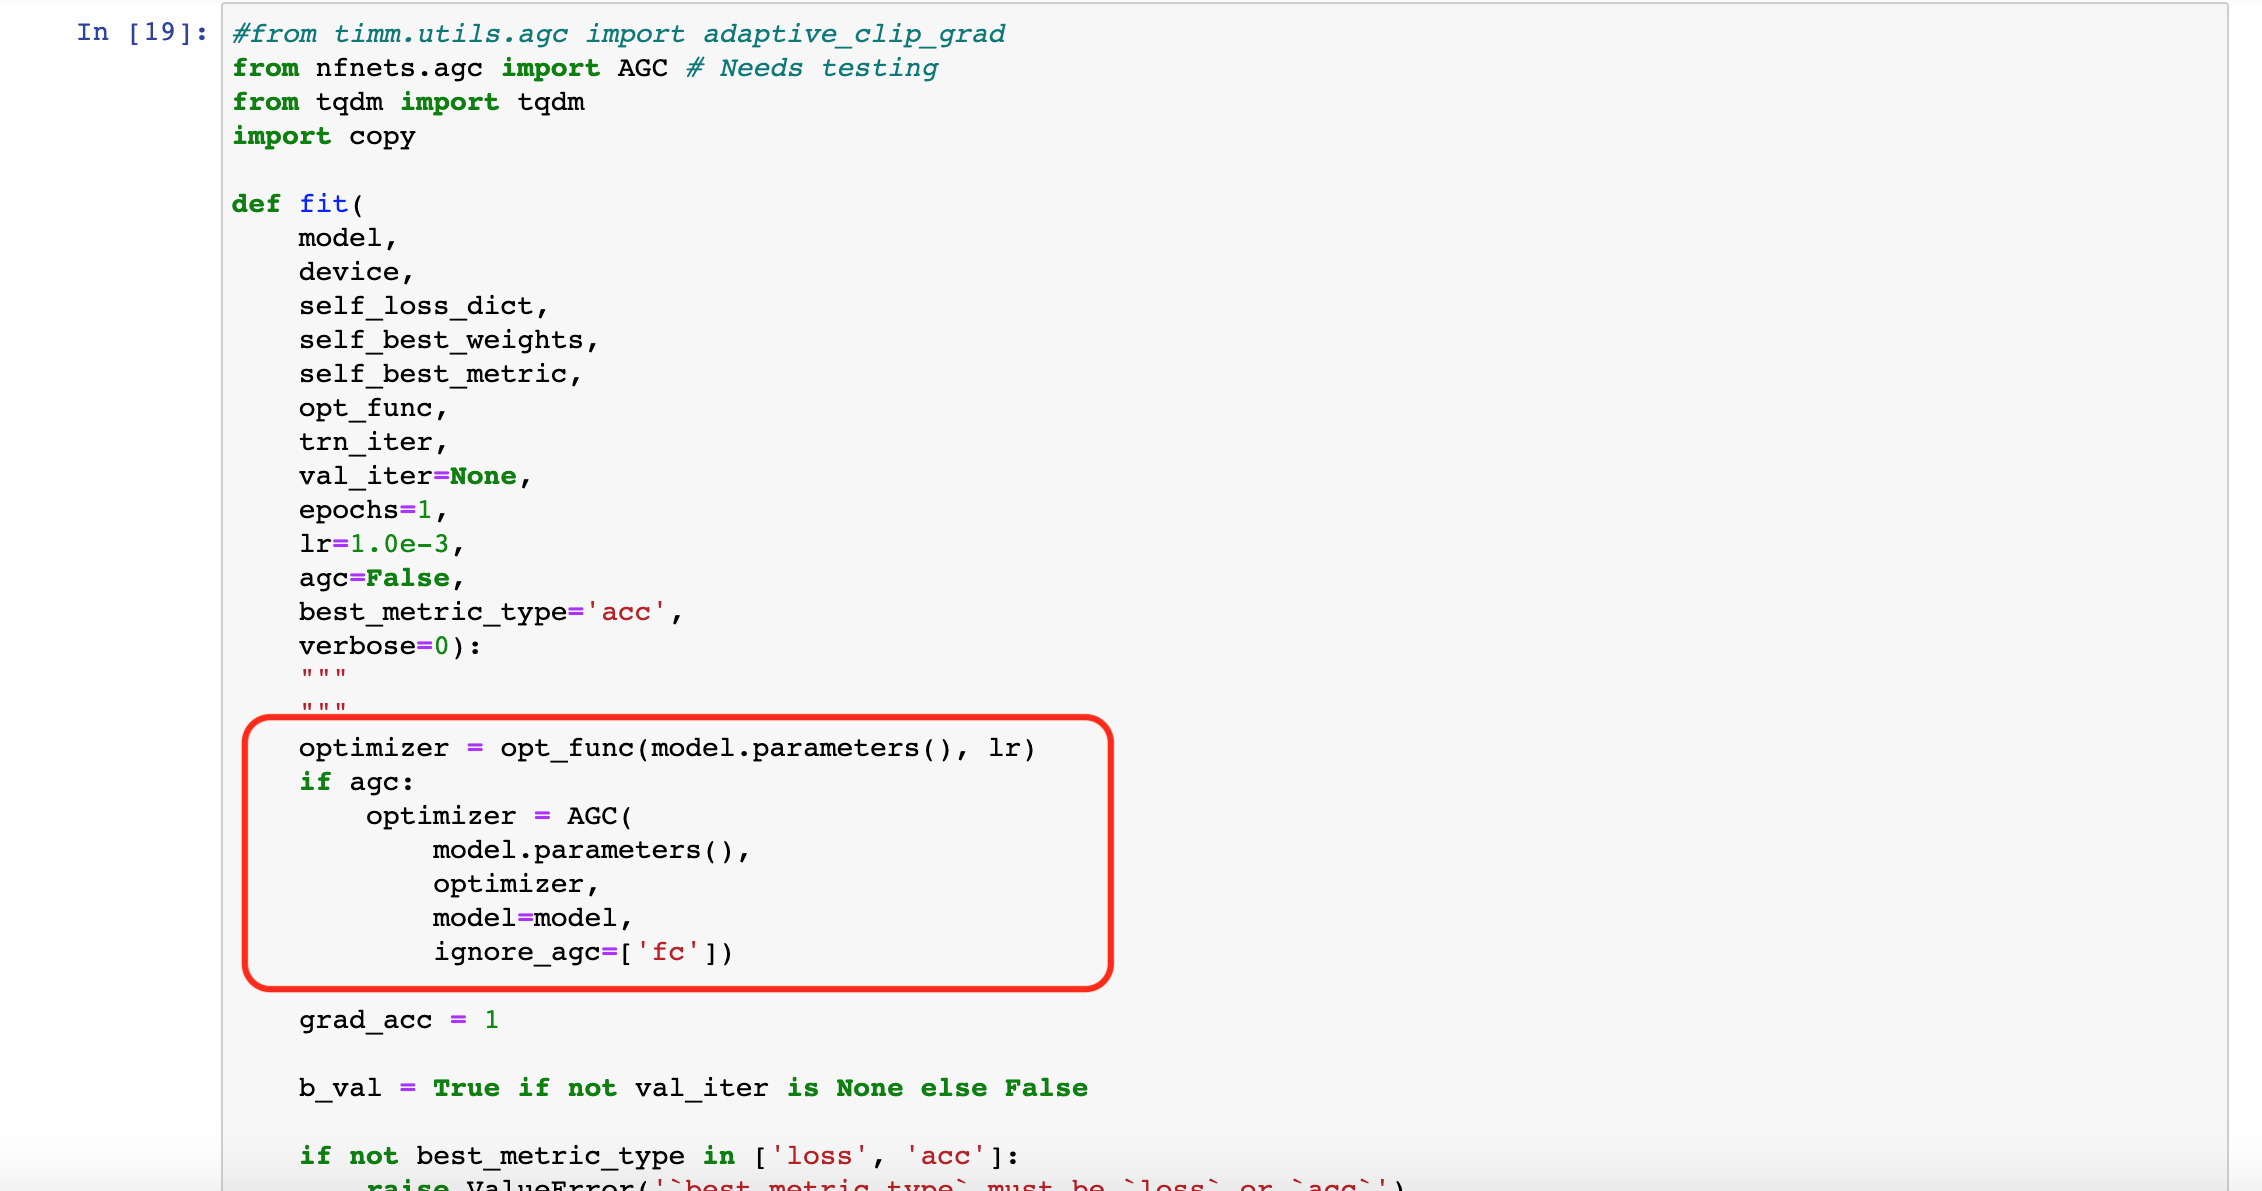
\includegraphics[width=0.63\textwidth]{images/nfnets-agc-vballoli-01.jpg}
  };  
\end{tikzpicture}

\vspace{5.0cm}

早速 AGC を使って学習してみましたが、やっぱりうまくいってないようで、
10 エポックで validation accuracy が 35.8\% ほど。

\begin{tikzpicture}[remember picture, overlay]
  \node[xshift=4.6cm,yshift=-5.5cm] at (current page.center){
    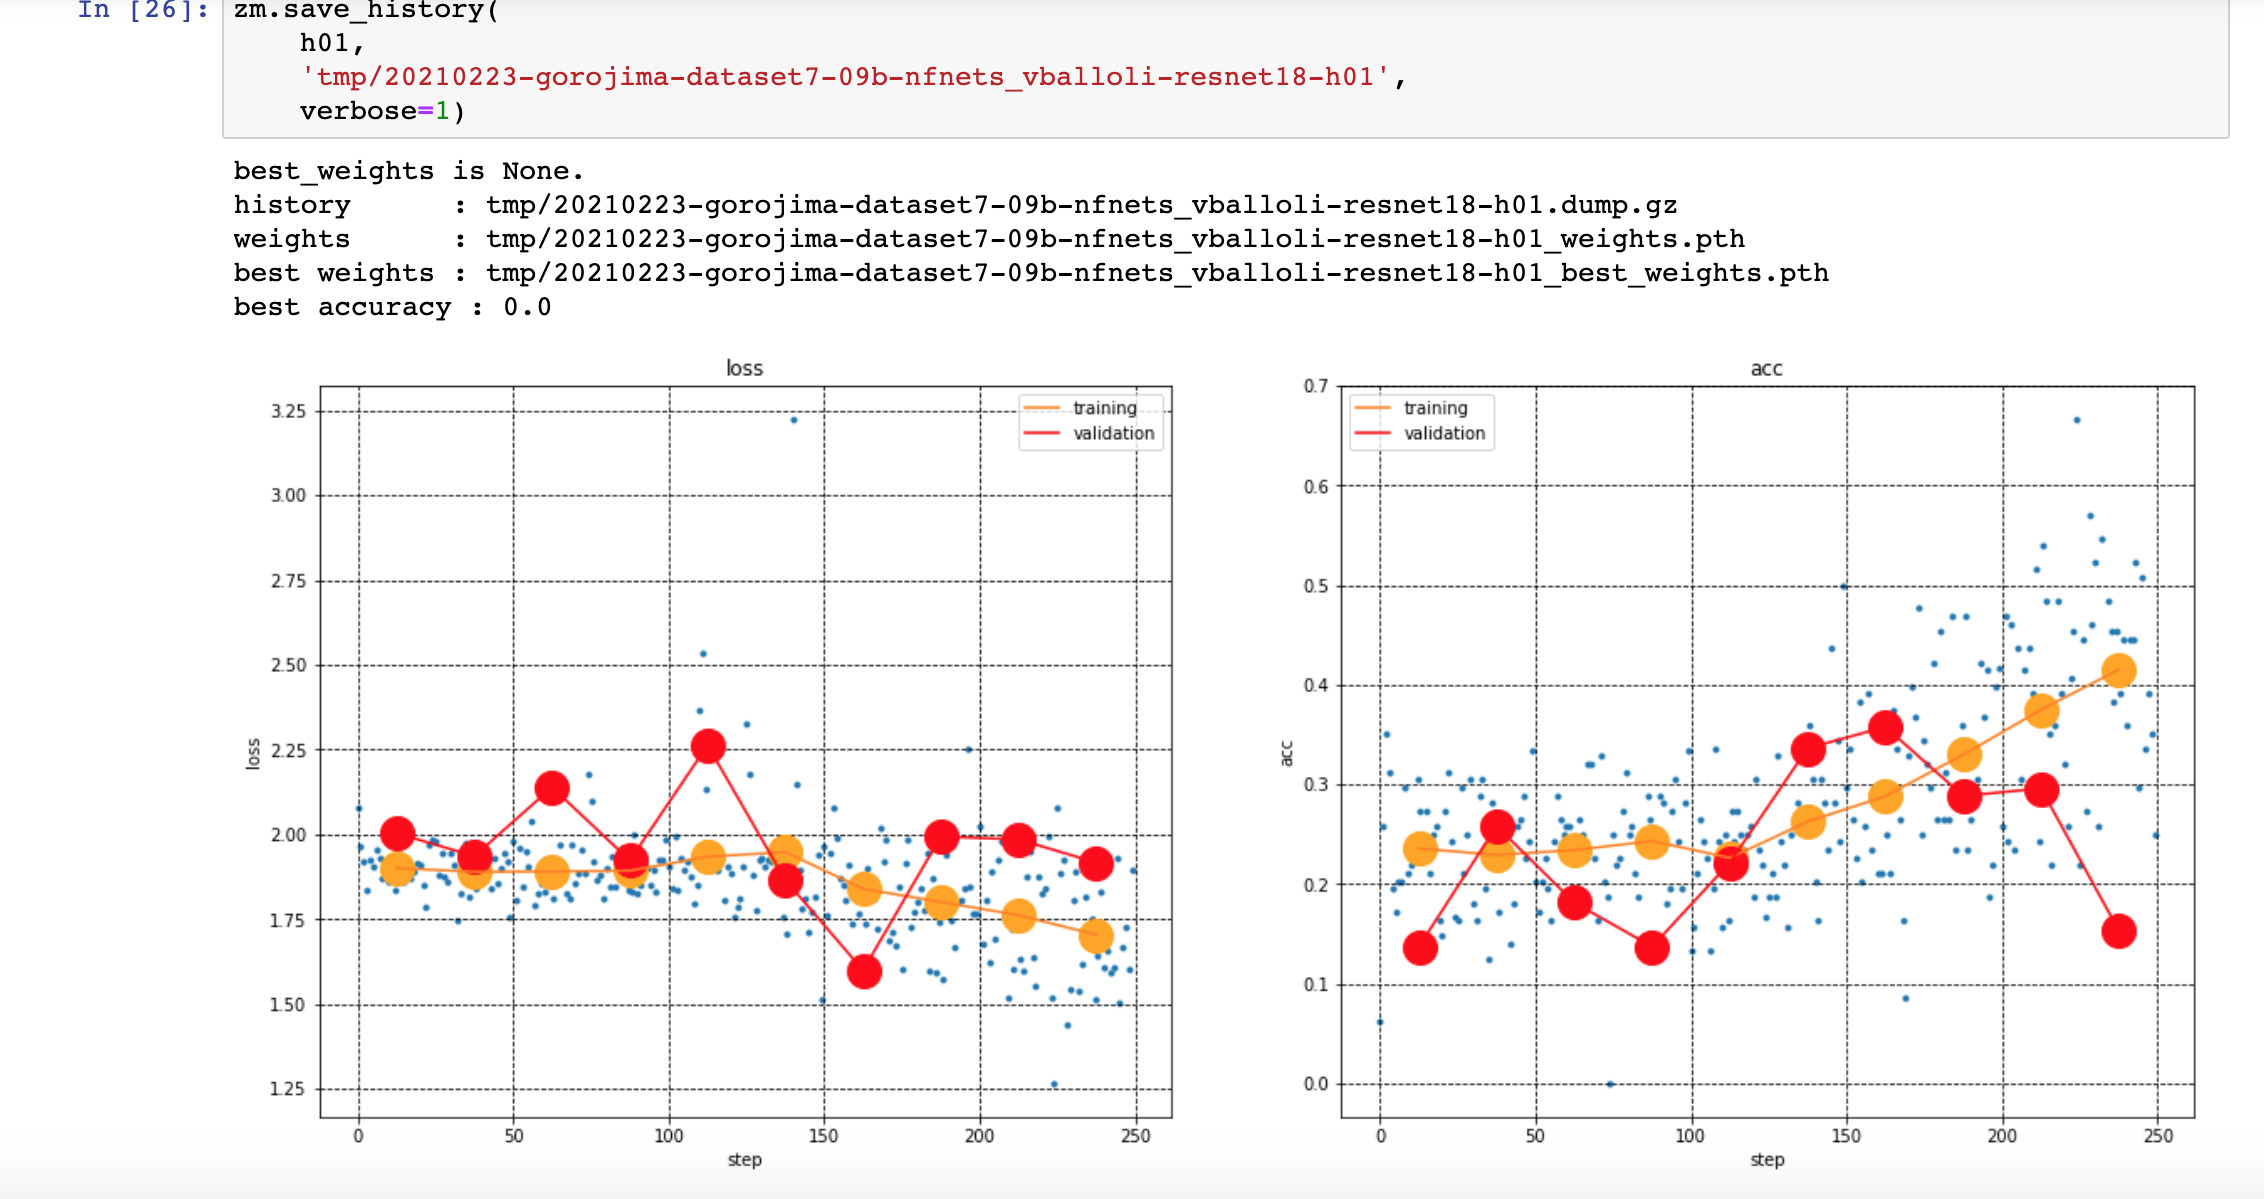
\includegraphics[width=0.63\textwidth]{images/nfnets-agc-vballoli-02.jpg}
  };  
\end{tikzpicture}

\vspace{5.0cm}

まだ何か根本的に理解できてないところがあるのでしょうか?

 %全角スペース

 %全角スペース

 %全角スペース


\section{AGC を使ってみる - timm 篇}
試行錯誤するときに、2つのオプションを持っていると言うのはいいことですね。
ということで、今手元にある実験台のもう一方の \texttt{timm} を今度は試してみます。
こちらは勾配を計算
\begin{quote}
  \texttt{loss.backward()}
\end{quote}
をした後で、パラメータの更新
\begin{quote}
  \texttt{optimizer.step()}
\end{quote}
をする前のところで、勾配を修正する関数
\texttt{adaptive\_clip\_grad()} を呼ぶという使い方をするようです。

\begin{tikzpicture}[remember picture, overlay]
  \node[xshift=-4.6cm,yshift=-2.5cm] at (current page.center){
    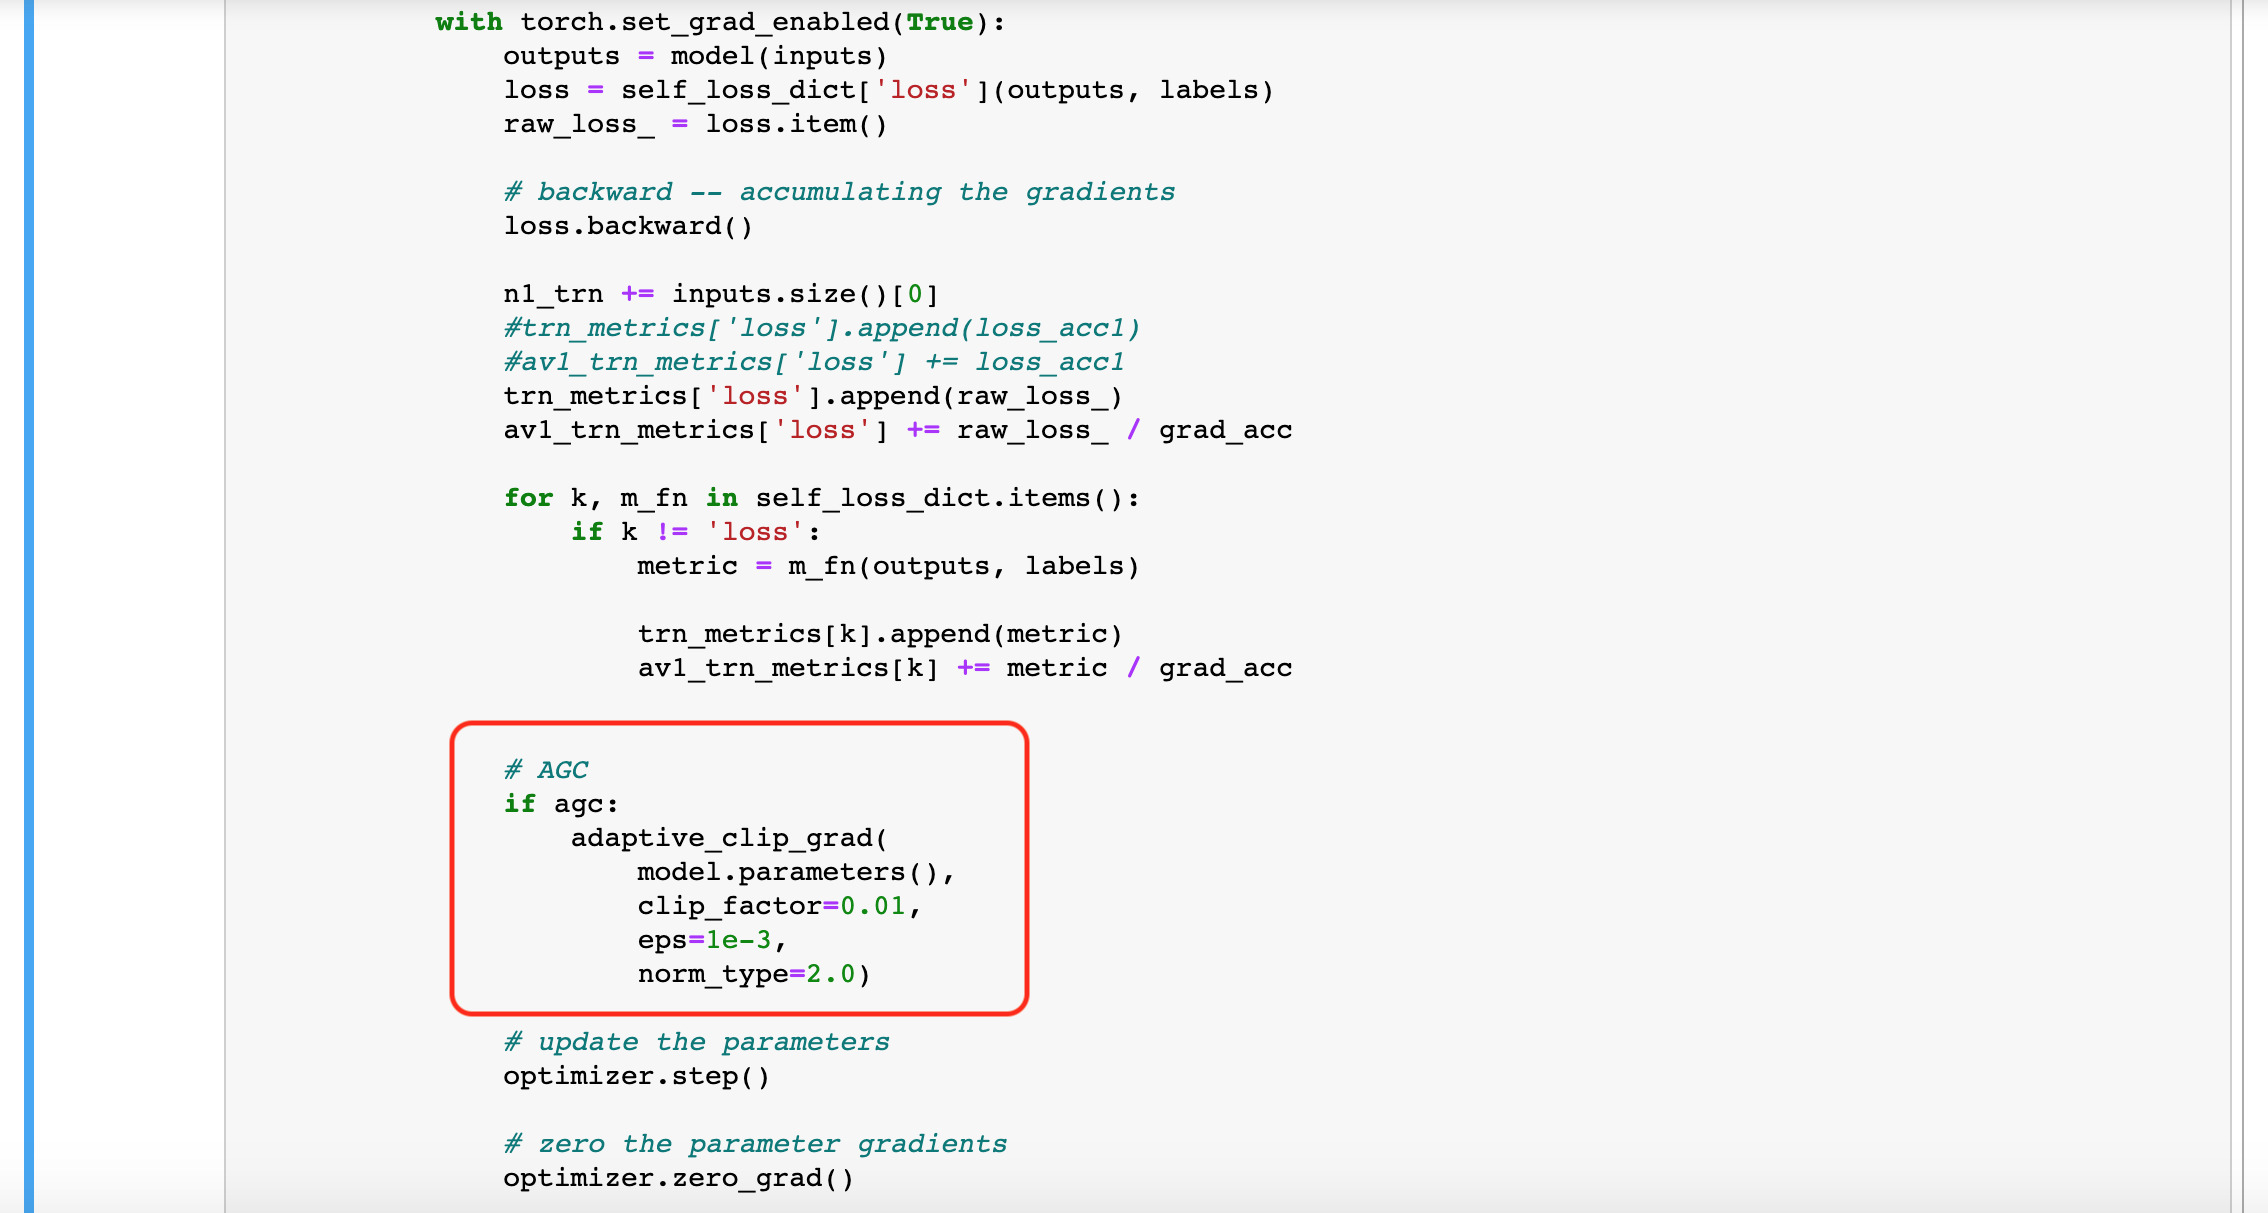
\includegraphics[width=0.63\textwidth]{images/nfnets-agc-timm-01.jpg}
  };  
\end{tikzpicture}

\vspace{5.0cm}

先と同様に AGC を使って 10 エポックほど学習したところ、
こちらは validation accuracy が 84.6\% まで上がりました。

\begin{tikzpicture}[remember picture, overlay]
  \node[xshift=-4.6cm,yshift=-10.0cm] at (current page.center){
    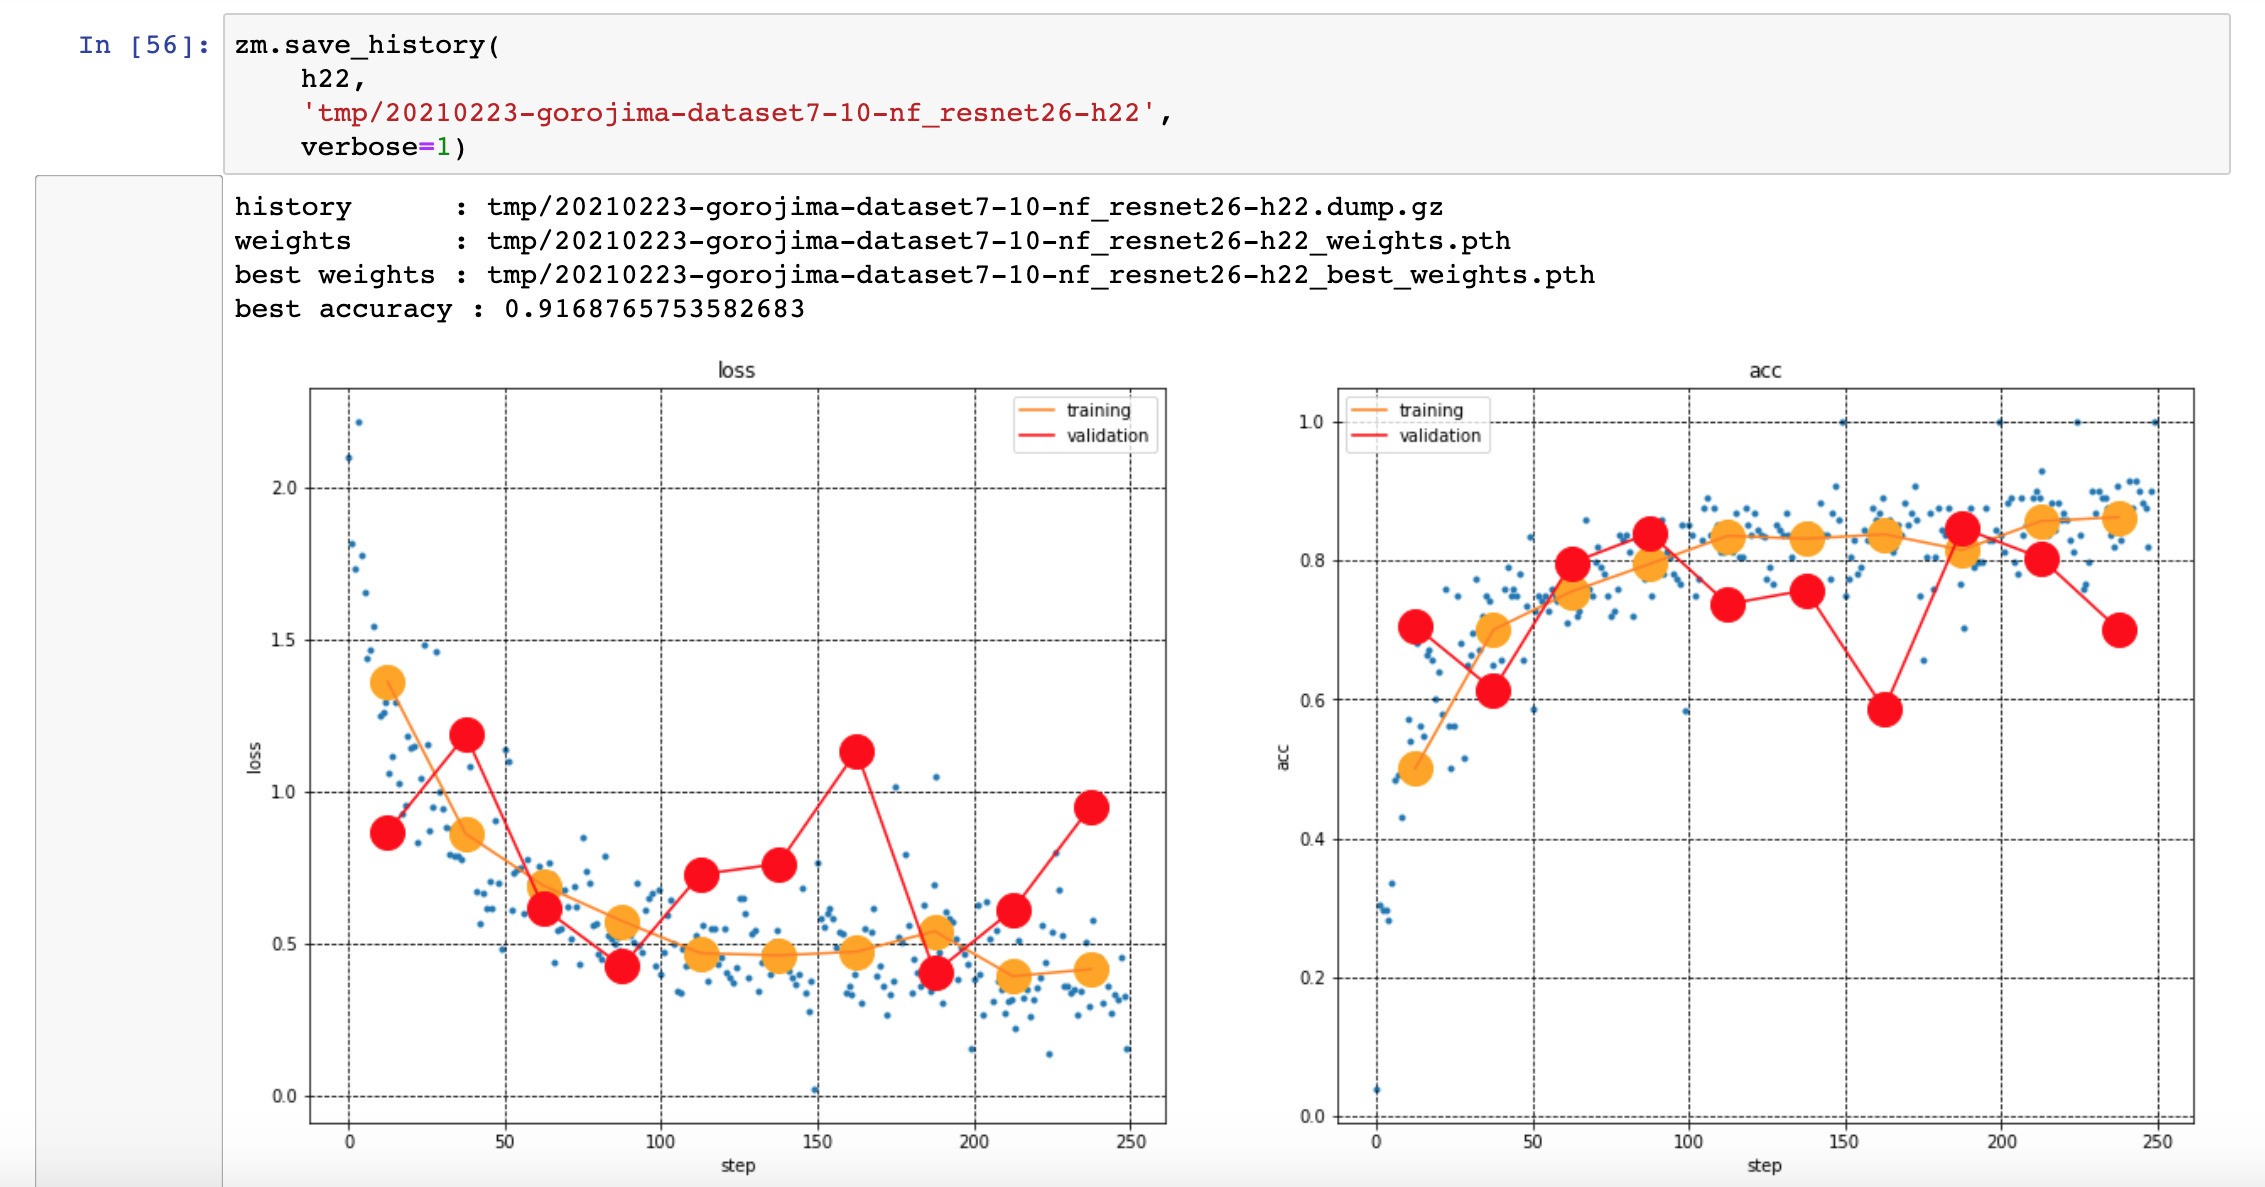
\includegraphics[width=0.63\textwidth]{images/nfnets-agc-timm-02.jpg}
  };  
\end{tikzpicture}

\vspace{2.8cm}

 %全角空白

しかし同じ学習ループを使って AGC を使わないで 10 エポック学習させた結果の方が
 85.1\% と僅かですがよくなりました。

\begin{tikzpicture}[remember picture, overlay]
  \node[xshift=4.6cm,yshift=5.0cm] at (current page.center){
    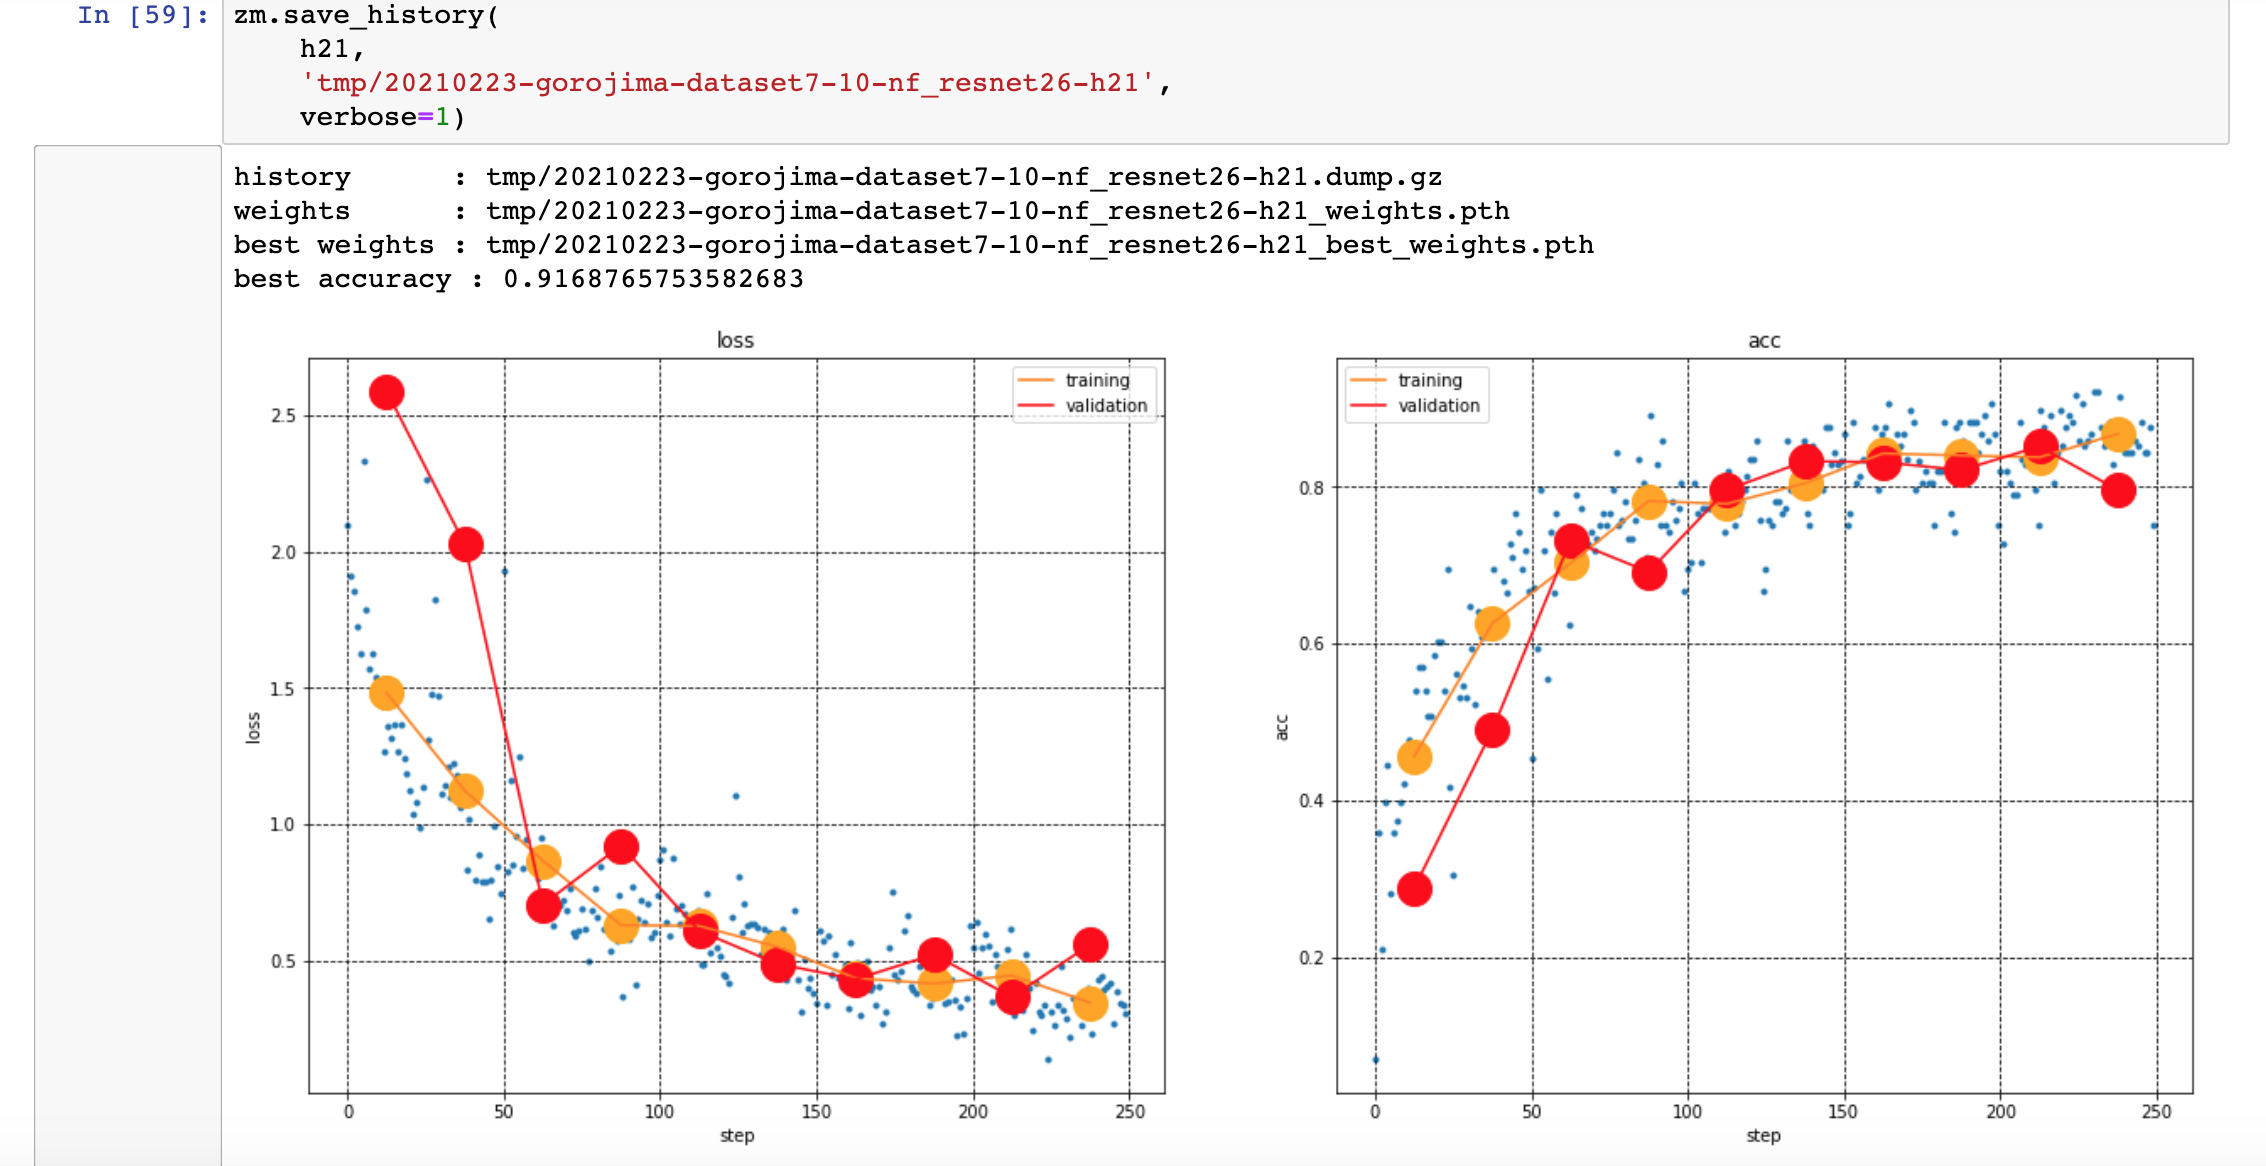
\includegraphics[width=0.63\textwidth]{images/nfnets-agc-timm-03.jpg}
  };  
\end{tikzpicture}

\vspace{4.5cm}

それに前に言ったとおり、このデータセットは単純な ResNet18 で $94\%$ を超えるので、
やはり期待していた SOTA の性能が出ているとは言えません。
関数 \texttt{adaptive\_clip\_grad()} はいくつかのパラメータを持っていて、
今はデフォルト値を使っていますが、
きちんとこれらの hyper parameter tuning しないと性能は出ないのかなと思います
(当たり前のことですね)。


\section{世間の情報を探してみる}
今回の調査は ZAF の自分の発表用に、深く掘り下げないでササっと調べて
「簡単に使ってみた、そして動いた」というデモをしたいという浅はかな考えで進めてきました。
その結果ここまでで紹介したように、そんな簡単な話ではないということを
身を以て味わったということです。
さて、世の中の人たちもみんなこんなに苦労しているのかどうか、
最後にちょっとググってみました。
出てきたページの1つ『TadaoYamaokaの日記』というブログサイトの
2021年2月20日のエントリー『将棋AIの実験ノート:Normalizer-Free Networks』
(\url{https://tadaoyamaoka.hatenablog.com/entry/2021/02/20/160626})
に、同じように NFNets を使おうとしている記事がありました。
コードは PyTorch で \texttt{timm} をベースに独自に書かれたもののようですが、
ResNet と比較して良い結果は得られなかったようです。
(そして、これをみて少し安心しました。)

一方で、今回の発端となった
\href{https://twitter.com/ZFPhalanx}{phalanx} さんですが、
その後フォローアップのツイート
(\url{https://twitter.com/ZFPhalanx/status/1364163567226773504})
をつぶやかれてます。

『ローマは一日にして成らず。』
今度きちんと論文を読み直して、
是非この画像分類 SOTA なモデル+学習方法をマスターしたいと思います。
(やっぱりパラメータ・チューニングかなぁ……)


\end{multicols}

\vspace{2cm}

\AddToShipoutPictureBG*{%
  \AtPageLowerLeft{%
    % Your background image here
    \includegraphics[width=\paperwidth,height=\paperheight]%
      {images/ZAM202102-p15-bg.jpg}
  }%
}%
\color{Maroon}
\begin{center}

\begin{tikzpicture}
\node[regular polygon, regular polygon sides=5, 
      minimum size=8cm,inner sep=0pt](h)  {}; 
\foreach \i [count=\next from 2] in {1,...,5}
  {% 
   \draw (h.corner \i) to [ornament=84] (h.corner \next);
   \pgfmathtruncatemacro{\next}{mod(\next,5)} }
\node[inner sep=6pt,yshift=1cm] (text) at (h.center){
  \Huge \sffamily \bfseries ZENKEI};
\node[inner sep=6pt] (text) at (h.center){
  \Huge \sffamily \bfseries AI};
\node[inner sep=6pt,yshift=-1cm] (text) at (h.center){
  \Huge \sffamily \bfseries MAGAZINE};
\end{tikzpicture}
\end{center}
\color{black}

\vspace{2cm}

% 4
\begin{tikzpicture}[remember picture, overlay]
  \begin{scope}[thick,rounded corners=8pt,
      xscale=1.3, xshift=-1.75cm, yshift=-3.5cm] at (current page.south)
  \draw (0, 2) -- (4.5, 2) -- (3.5, 0) -- (5, 0);
  \draw (5, 0) -- (6, 2) -- (7, 0);
  \draw (7, 0) -- (8, 0);
  \draw (4, 0.8) -- (8, 0.8)
    -- (8.7, 2) -- (9.7, 0) -- (10.7, 2) -- (10.7, 0) -- (14, 0);
  \end{scope}
\end{tikzpicture}

\newpage

\AddToShipoutPictureBG*{%
  \AtPageLowerLeft{%
    % Your background image here
    \includegraphics[width=\paperwidth,height=\paperheight]%
      {images/ZAM202102-cover-2-v2.jpg}
  }%
}%
\thispagestyle{empty}
\begin{tikzpicture}[remember picture, overlay]
  \node[xshift=2.12cm,yshift=-2.93cm] at (current page.north west){
    %\textcolor{white}{\bfseries \thepage}
    {\bfseries \thepage}
  };  
\end{tikzpicture}
\begin{tikzpicture}[remember picture, overlay]
  \node[xshift=-1.0cm,yshift=0.3cm] at (current page.south east){
    {\small \sffamily illustration}
  };  
\end{tikzpicture}

 % 全角スペース

\newpage

\AddToShipoutPictureBG*{%
  \AtPageLowerLeft{%
    % Your background image here
    \includegraphics[width=\paperwidth,height=\paperheight]%
      {images/ZAM202102-cover-3-v2.jpg}
  }%
}%
\thispagestyle{empty}
\begin{tikzpicture}[remember picture, overlay]
  \node[xshift=-2.05cm,yshift=-2.93cm] at (current page.north east){
    %\textcolor{white}{\bfseries \thepage}
    {\bfseries \thepage}
  };  
\end{tikzpicture}

\begin{tikzpicture}[remember picture, overlay]
  \node[xshift=1.0cm,yshift=0.3cm] at (current page.south west){
    {\small \sffamily furukawa}
  };  
\end{tikzpicture}
 % 全角スペース

\newpage

\chapter{『月刊 ZENKEI AI MAGAZINE』創刊}
\label{ch:zam}

\begin{tikzpicture}[remember picture, overlay]
  \node[xshift=2.12cm,yshift=-2.93cm] at (current page.north west){
    \textcolor{white}{\bfseries \thepage}
  };  
\end{tikzpicture}

ZENKEI AI FORUM (ZAF) 2021年1月で『技術書典10』を振り返る中で
いきなり雑誌創刊を宣言し、毎月のイベント時に、前月の内容を書籍化した月刊紙を
(オンラインで)発行することにしました。
この1月の ZAF の内容を、当日発表した(わたしを含む)3人が
その後1ヶ月を掛けて書き上げ、
ZAF 2021年2月のイベントにおいてこの記念すべき
ZENKEI AI MAGAZINE (ZAM) の創刊第1号を発刊しました。
ここでは ZAM 創刊に至る流れと、創刊号の共同執筆の内容を、まとめたいと思います。


\begin{multicols}{2}


\section{前兆}
長いもので、ZAF の前身の ZENKEI AI SEMINAR がスタートしたのが 2017 年なので、
この AI 技術の地域コミュニティ活動も既に3年を超えることになります。
わたし自身、要領が良くなかったり、手が早くなくスピード感に劣るということもあるので、
やると決めたことはきちんとやり切りたいし、
やりっぱなしにしたくないと思ってます。
当たり前のことですが、人生は有限なので、
瞬間々々意味のあることをやりたいし、
意味のあることはきちんと形にしておきたい。
そういう意味の「責任感」を持って、少なくとも自分の手の届く範囲のことがらは
やっていきたいなと思っています。

そういう偉そうなことを言わなくても、
単に、ふと自分はどれくらい頑張ったかなと振り返ってみたとき、
やってきたことがきちんと形になってたらいいなと時々思います。

実際にこれまでも ZAF のコンテンツ化、アーカイブ化は意識的に行ってきました。
具体的には
\begin{itemize}
\item YouTube のアーカイブ
\item スライド、資料などのアーカイブ
\item コンテンツのポッドキャスト化 - ZENKEI AI Podcast (ZAP)
\end{itemize}
などは既に行っています。
(ZAP は、気付くと 2020年8月の途中で止まってますね。)
一方、今のところできてないこと、やってないことには
\begin{itemize}
\item ウェブ化(オンライン・フォーラムだけ)
\item 書籍化(メンバーの個人プロジェクトはスタート)
\end{itemize}
が挙げられます(他にも沢山あると思います)。


\section{妄想と共感}
そんな気持ちを持ちながら、
ZAF の活動については、その時々に、あれこれ考えていて、
常に形を変えたり大きく広がったりしていると思います。
そういう流れの中の最近の「ふわっ」としたイメージをまとめられる範囲でまとめると、
以下のような言葉になります:
\begin{itemize}
\item ZAF は(地域)コミュニティを目指している。
\item コミュニティとは「主体的な人」の集まりであり、
  それはつまり「秘密結社」だ(瀧本哲史)
\item (秘密)結社は同人であり、
  同人といえば同人誌である
\item 人は、たのしそうなイベントに集まる
\item 思考やアイデアは、おもしろそうな雑誌のまわりに集まる
\item 「たのしそうなイベント」が ZAF である
\item 「おもしろそうな雑誌」が ZAM である!
\end{itemize}
なんか、いい感じに発展してきた気がします。

そんなことを感じながら日々あれこれ考えています。
そんな中、最近、共感したツイートがありましたので、
ここで2つほど紹介したいと思います。

\AddToShipoutPictureBG*{%
  \AtPageLowerLeft{%
    % Your background image here
    \includegraphics[width=\paperwidth,height=\paperheight]%
      {images/ZAM202102-p19-bg.jpg}
  }%
}%
\subsection{静かな活動}
1つ目は
``{\bfseries Jazz The New Chapter}'' という
%(きちんとした)
(わたしたちのような同人誌ではなく、きちんとした)
商業雑誌を運営している柳樂光隆さん
(\href{https://twitter.com/Elis_ragiNa/}{Elis\_ragiNa})
のツイート
(\url{https://twitter.com/Elis_ragiNa/status/1361522687621828608})
です。
\begin{quotation}
  \noindent
  個人的には「自分で枠を買ってやる」ってのと、
  「タイムリーじゃないことをやれる場所を作る」ってのが面白いと思ってて、
  現状、そういう場所が少ないって部分での提案でもある。

  プロモーションや広告、バズから離れるための試み。
  パーソナルな音楽との付き合いをシェアできる場所というか、ね。

  とはいえ、TUNEINは世界中で使われてるアプリだから、
  実はかなりの聴取者がいて、かなり驚く。

  radikoだと日本の番組しか聞けないから、
  海外の人が偶然聴くみたいなことはなかなか起きない。

  リアルタイムのみで不便なアプリだが、
  想像してたよりかなり可能性を感じて、好きになってる。
\end{quotation}
これは地方 FM ステーションの時間枠を自分で買って、
自分の好きな音楽を流そう、という話(なのかな?)。
仕組み的には企業がやっていることを
\ruby{私}{わたくし}がやるということですが、
「プロモーションや広告、バズから離れるための試み」
とあるように目的は明らかに違いますよね。

本来個人的なものであるはずの SNS
(という考え方自体が、あまりにも na\"{i}ve なんでしょう)
が、気付くと、大企業がアテンションを集めるロジックをそのまま
個人レベルで行ってる「やかましい」世界になっていて、
そういう個人の自発的な活動で結局プラットフォームを握っているところが商売しているという
ビジネスモデルが成立している訳ですが、
それで失われる(あるいは価値を認められない)しかし大切な「静かな活動」を
どのように育んでいくのか、という問題意識を、わたしも
(ZAF の活動などを通じて)考えています。
	  
ちなみに ZAP も TuneIn
(\url{https://tunein.com/podcasts/Technology-Podcasts/ZENKEI-AI-Podcast-p1313880/}) で聞けます!
もちろんその他のポッドキャスト・サービスからも聞けます。
詳しくは ZAP サイト \url{https://zenkei.seesaa.net/} をご覧ください。


\AddToShipoutPictureBG*{%
  \AtPageLowerLeft{%
    % Your background image here
    \includegraphics[width=\paperwidth,height=\paperheight]%
      {images/ZAM202102-p20-bg.jpg}
  }%
}%
\subsection{アンドレ・ヴェイユ}
もう1つのツイートは「数学の歩みbot」さん
(\href{https://twitter.com/Auf_Jugendtraum}{Auf\_Jugendtraum})
の以下のツイート
(\url{https://twitter.com/Auf_Jugendtraum/status/1361429835600470017})
です。
\begin{quotation}
  \noindent
  共同研究に対する忠告を3つ.\\
  先ず over organize し過ぎないこと.\\
  次に,常に,あらゆる種類の失望に対し備えていなければならないこと.\\
  失望は共同研究の一部であると考えるべきである.\\
  第三にアイデアは集団から生まれるのではなく 個人から生まれるということだ.\\
  (アンドレ・ヴェイユ)
\end{quotation}
研究者(数学者)が共同研究をする上での心得ですが、
上司が部下に仕事を振る時とか、
自分の手が回らない時に助けをお願いする時など、
幅広く応用できるなと深く肯きました
(実践できているとは言いませんが)。
特に今回一番「そうだよな」と思ったのは最後の項。
本来弱い存在である個人(および個人のアイデア)を
どのように\ruby{拾}{ひろ}い上げるか、それを継続的に系統的に行っていくのか、という点。
エンジニアという人種はともすると\ruby{人月}{にんげつ}でものごとを計画しますが、
ここが分かってないんだよな、と。(もちろん、タスクの内容によりますが。)


ところで、わたしが\ruby{殊更}{ことさら}に
このツイートに目が行った理由は「アンドレ・ヴェイユ」です。
とは言っても(わたしは数学には詳しくはないので)彼の数学者の業績というのは
何も知らないんですが、昔(何時ごろのことか忘れてしまいましたが、大学院の頃だと思います)
ネットで見た彼の言葉(でありエピソードである)
\begin{center}
  \textgt{\large 数学は体力だ!}
\end{center}
が当時も、そして今もまだ強烈に記憶に残っているからです。
改めてググってみると、当時のわたしが目にした記事(が転載されたもの)が見つかりました。
みなさんも是非読んでみてください。
『数学は体力だ!(木村達雄)』
(\url{https://nc.math.tsukuba.ac.jp/column/emeritus/Kimurata/})
です。
しかし改めて考えると、数学だけでなく人生は全て最終的には体力ですね。
あと『体が資本』という言葉もあります。こういう言葉が響くようになる、
ということが自分が年を取った証拠なのでしょうが、
まだまだ若いみなさんも意識した方がいいですよ、と(いつもの)
余計な事を言ってしまいました。

 % 全角スペース

\section{閃き}
\begin{tikzpicture}[remember picture, overlay]
  \node[xshift=-4.6cm,yshift=5.0cm] at (current page.center){
    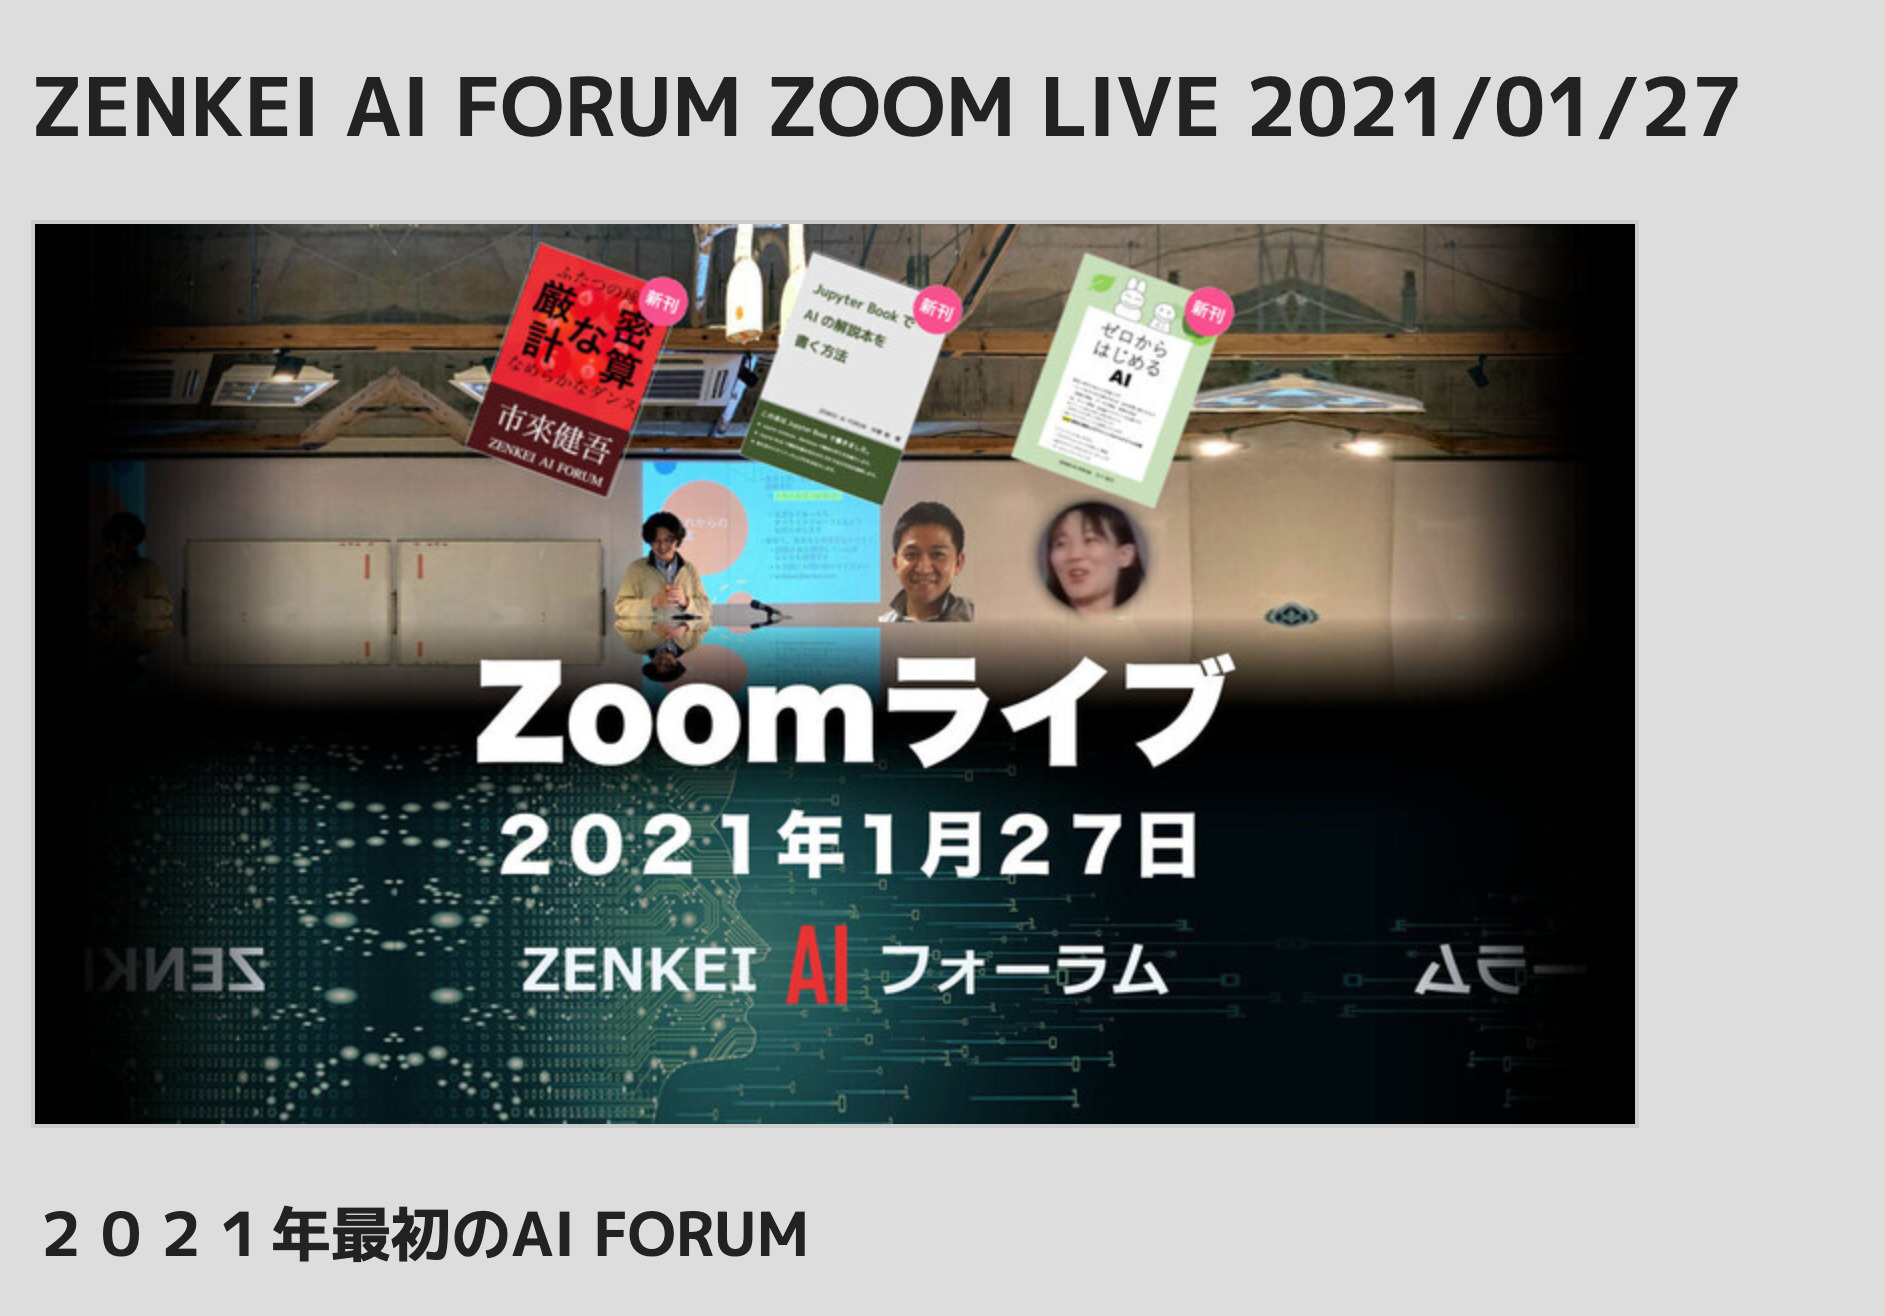
\includegraphics[width=0.63\textwidth]
      {images/ZAF202101-01.jpg}
  };  
\end{tikzpicture}

\vspace{6.0cm}

こんなことをあれこれと、あてもなく考えながら迎えた
前回 2021 年最初(2021年1月27日開催)の ZAF の自分の発表を準備していたときに
閃きました。
「雑誌を作ろう」と。
(わたしは定期的に「ひらめいた!」と叫んでいますね。)

\begin{tikzpicture}[remember picture, overlay]
  \node[xshift=-4.6cm,yshift=-5.7cm] at (current page.center){
    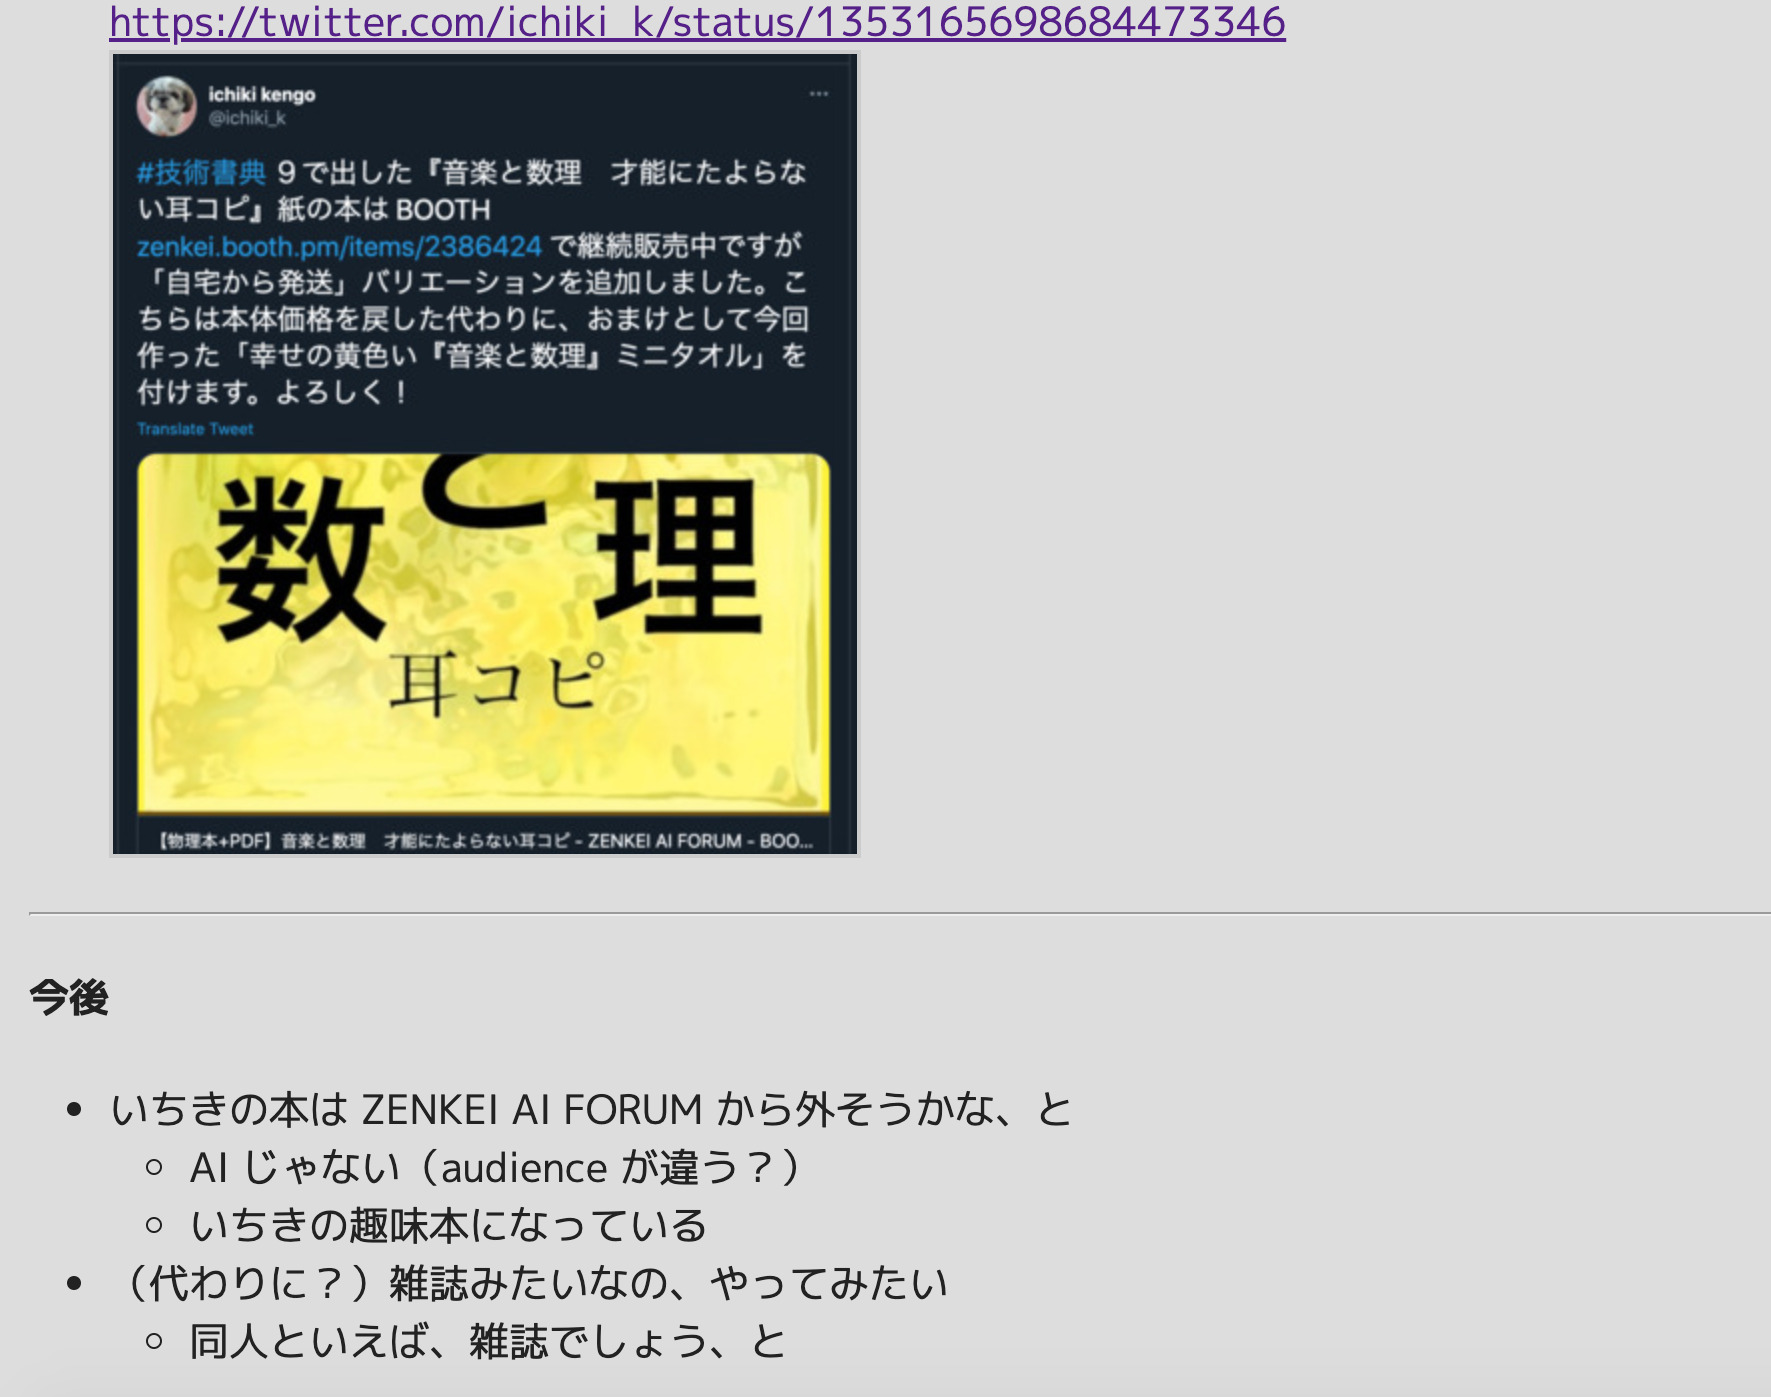
\includegraphics[width=0.63\textwidth]
      {images/ZAF202101-02.jpg}
  };  
\end{tikzpicture}

\vspace{6.8cm}

\AddToShipoutPictureBG*{%
  \AtPageLowerLeft{%
    % Your background image here
    \includegraphics[width=\paperwidth,height=\paperheight]%
      {images/ZAM202102-p21-bg.jpg}
  }%
}%
自分の子供のころからのことを振り返ると、
今の自分って実際のところ雑誌で育ってきたんだなと思います。
具体的に読んできた、影響を受け刺激を受けてきた雑誌を挙げると、
\begin{itemize}
\item 誠文堂新光社『\textgt{子供の科学}』
  (真ん中に厚紙の飛行機が付いてましたね)
\item 『\textgt{ラジオの製作}』
  (わたしは『初歩のラジオ』派ではありませんでした)
\item 『\textgt{月刊 \bfseries I/O}』
  (パックマンとかのバイトダンプを手で打ち込んでたな)
\item 『\textgt{トランジスタ技術}』
  (昔の分厚かった頃のやつ、硬派でしたね)
\item 『{\bfseries UNIX MAGAZINE}』
  (大学の頃、UNIX 系の情報源といえばこれしかなかった)
\item 『{\bfseries Jazz Life}』
  (譜面がたくさん載ってるJazzの本はこれしかなかった)
\end{itemize}
などがすぐに出てきます。
こうして並べてみるとさすがに時代を感じますが、
同時に、今本屋に行って手に取る雑誌にないものがあるように思います。
わたしが好きだったこれらの(当時の)雑誌に共通して言えることは、
読者を子ども扱いしない、素人扱いしない、という姿勢です。
逆に言うと、今の雑誌(に限らず、メディア一般と言ってもいいのかな)は
「分かりやすく」「受け入れられやすく」ばかりを優先し、
本質的に大切な、しかし説明するにはいろいろと面倒な事柄を
(意図的か否かは別として)結果的にスキップしていて、
歯ごたえの無いふわふわして真っ白な食パンみたいになってる気がします。
これでは読者は育たないだろうな、と思います。

脱線しました。
いずれにせよ ZAF 2021年1月のイベントで
\begin{center}
  \Large {\gtfamily\bfseries ZAM 爆誕!}
\end{center}
しました(少なくとも「やるぞ」ということだけは)。

 % 全角スペース

\end{multicols}

\AddToShipoutPictureBG*{%
  \AtPageLowerLeft{%
    % Your background image here
    \includegraphics[width=\paperwidth,height=\paperheight]%
      {images/ZAM202102-p22-bg.jpg}
  }%
}%
\begin{tikzpicture}[remember picture, overlay]
  \node[xshift=0cm,yshift=-5.4cm] at (current page.north){
    
\includegraphics[width=1.1\textwidth]
      {images/aiforum_20210129.png}
  };  
\end{tikzpicture}

\vspace{3.1cm}

\begin{center}
オンラインフォーラム 1 月 29 日の古川さんの投稿\\
(\url{https://forum.ai.zenkei.com/t/topic/340/43})
\end{center}

\begin{multicols}{2}

\section{計画}
``How to start a movement''
という約 10 年前の 2010 年の TED の有名な講演の1つ、
Derek Sivers によるわずか 3 分ほどのとても明快なビデオがあります
(\url{https://youtu.be/V74AxCqOTvg})。
まだ見たことのない人には是非人生の 3 分を投資することをお勧めします。
そこでのフォーカスは「どうやって」活動を始めるか、
その活動を成功に導く大切なポイントは何か、でした。
今ここで「爆誕!」と言っている ZAM もそういった「活動」の1つです。
「どうやったら成功するか」というのは気にならないと言えば噓になりますが、
今の時点ではむしろ、どうやったら継続的な、
今風に言えば sustainable な活動になるのかにわたしの関心はあります。
何かを始めること(ゼロを1にすること)は
それ自体大変と言えば大変ですが、
気合いとか勢いで結構できてしまうものです。
それに比べて、そうやって勢いで始めた活動を継続することは、
始めることに比べるとずっと大変なことだと思います。

難しい問題に取り組むには計画が必要です。
ということで始めるにあたってあれこれと構想を練ってみました。
まず考えたのは「無料版」と「有料版」を分けるという考えです。
「無料版」は、
\begin{itemize}
\item 月刊で、無料で誰でも読める形で、全世界に公開
\item 内容は、毎月開催している ZAF の内容がベース
\item 発行は毎月の ZAF 開催日で、前月の内容の ZAM を出す
\end{itemize}
という形。
既に毎月イベントを運営してきた経験があるし、
イベントのコンテンツはあるので、
それほど無理をしなくても実施できるでしょう。
ZAF のイベントが基本的にオープンなイベントなので
必然的に『月刊 ZAM』もオープンアクセスな雑誌にします。

ただそれだけだと、せっかく「雑誌」という媒体を作るのに
もったいない気がしました。
雑誌といえば「連載コーナー」ですよね。
ZAF サークルとしてこれまで2度の『技術書典』で4冊の本を
企画、出版してきました。
これらは「単行本」であり、執筆者それぞれのソロ活動的な側面があります。
執筆へのハードルという意味では、
雑誌への寄稿という形にすると一度の執筆の分量が減るので、
その結果サークルメンバーの執筆活動への参入を促すだろう
という思いもあります。
「有料版」は、
\begin{itemize}
  \item 季刊(あるいは年数回)で刊行
  \item 無料版の月刊の内容をまとめる
  \item 書き下ろしコンテンツなどを追加
  \item タイミングが合えば『技術書典』などのイベントで販売
\end{itemize}
というイメージです。
刊行が進んで書き下ろし連載の内容が増えてきたら、
それを「単行本」としてまとめて出版することもできます。
「有料版 ZAM」の売り上げは ZAF に、
単行本の売り上げは(これまで通り)執筆者に還元すれば、
よい循環ができるかなと思っています。


\section{共同執筆}
『ZAM 創刊』を 2021年1月の ZAF で(なんら根回しなしにいきなり)発表しました。
成り行き上、言い出しっぺの法則でわたしが編集長に就任することにして、
早速1月の ZAF の内容をベースに創刊号の執筆、編集作業を開始しました。

\begin{tikzpicture}[remember picture, overlay]
  \node[xshift=-4.6cm,yshift=-6.8cm] at (current page.center){
    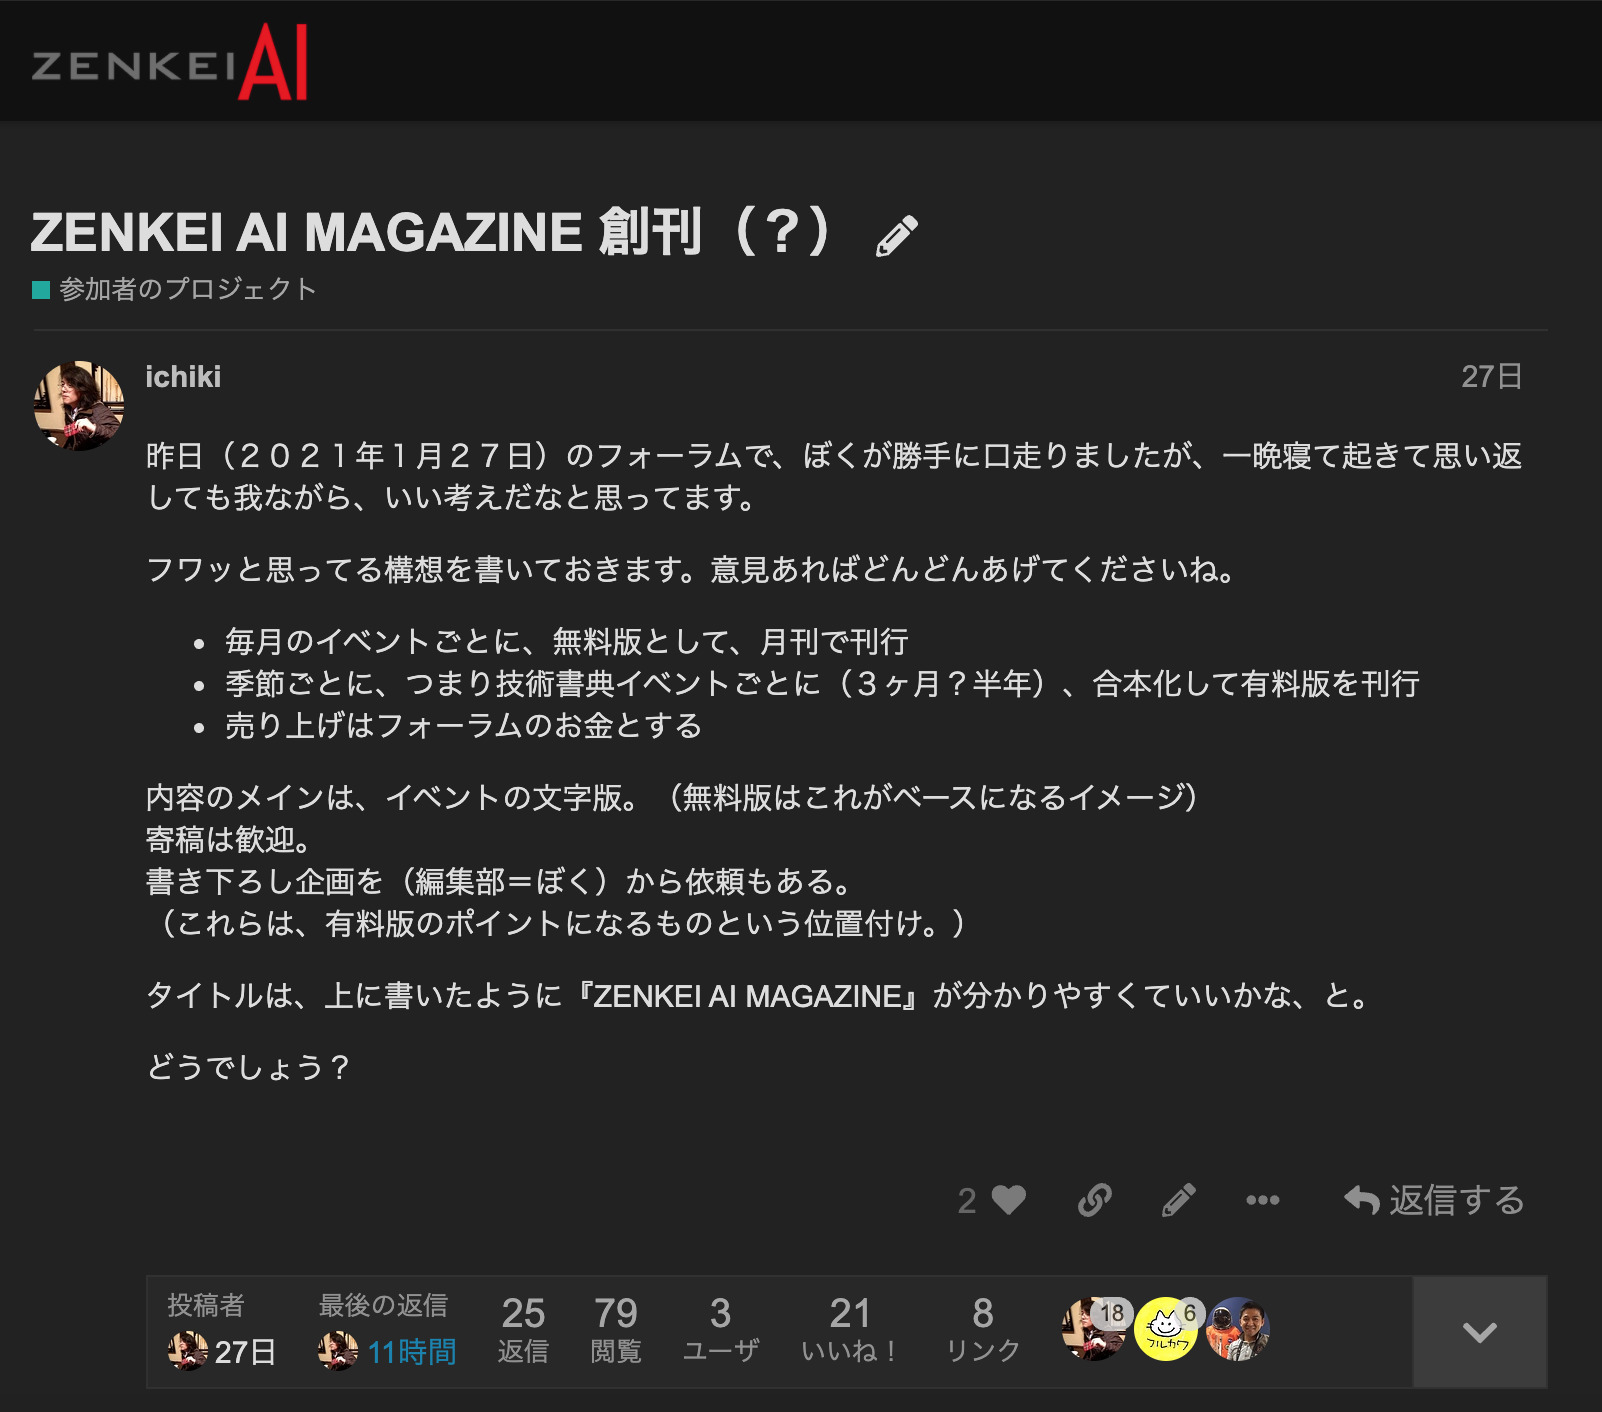
\includegraphics[width=0.63\textwidth]
      {images/online-forum-01.jpg}
  };  
\end{tikzpicture}

\vspace{7.2cm}

 % 全角スペース

まずオンラインフォーラムにスレッドを作りました。
(\url{https://forum.ai.zenkei.com/t/topic/349})
次に『月刊 ZAM』創刊号の執筆者、つまり
ZAF 1月の講演者の二人、古川さんと中野さんに早速原稿依頼しました。

\begin{tikzpicture}[remember picture, overlay]
  \node[xshift=4.6cm,yshift=3.5cm] at (current page.center){
    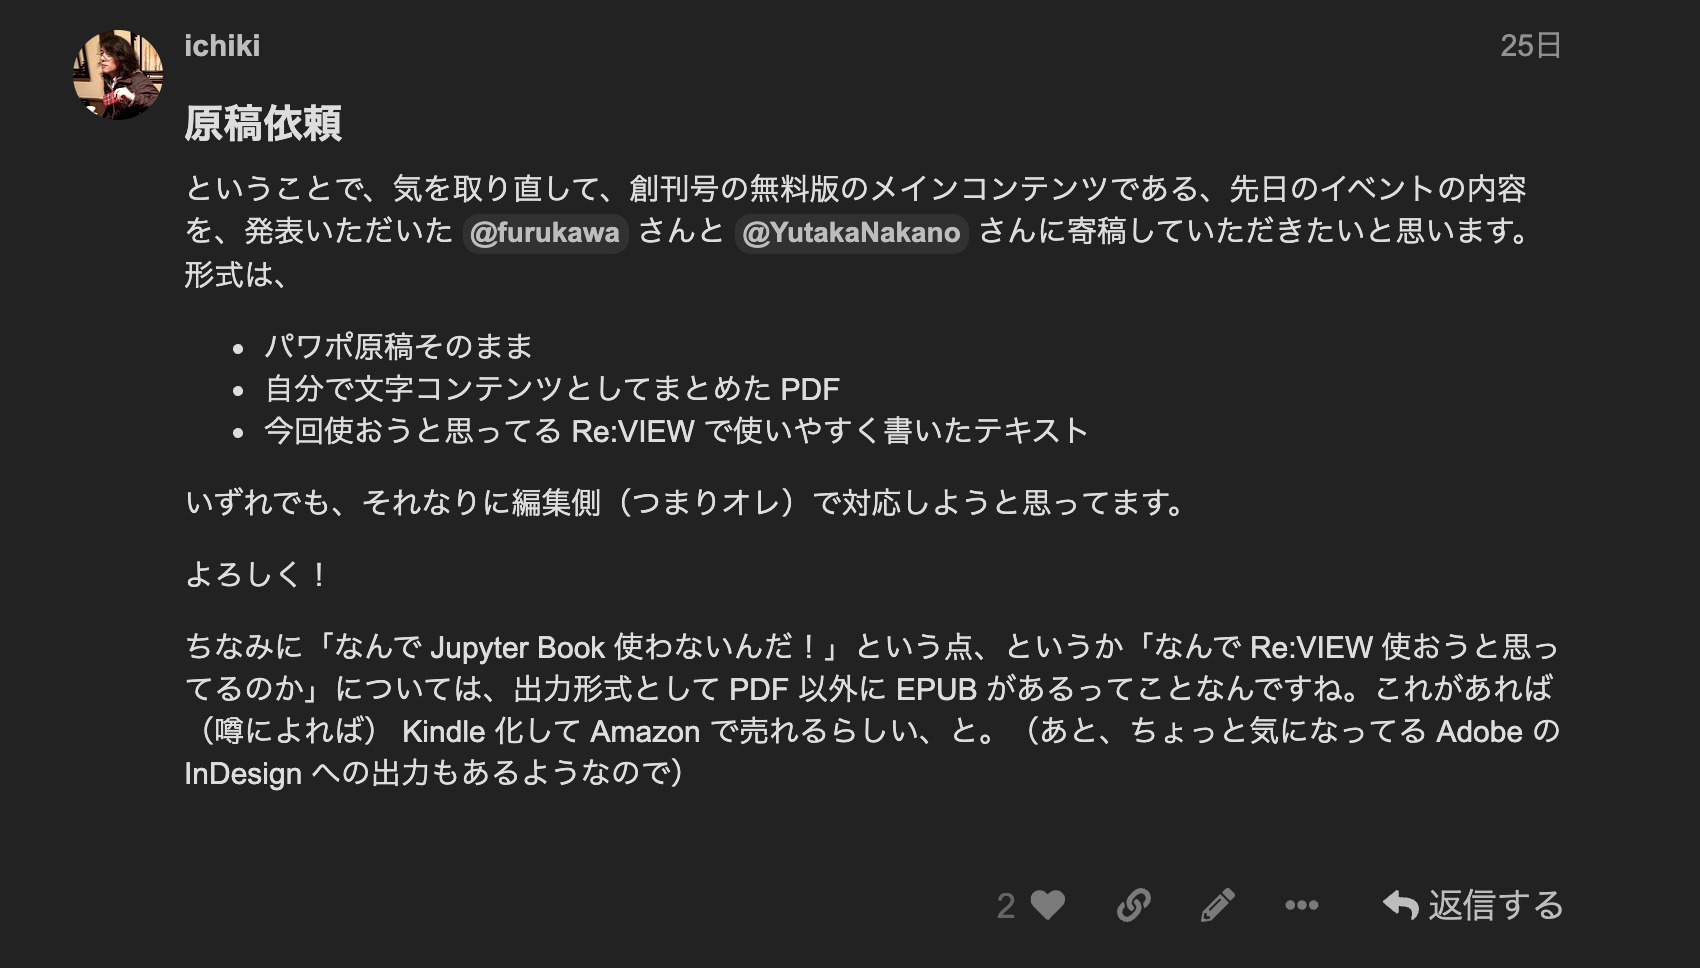
\includegraphics[width=0.63\textwidth]
      {images/online-forum-02.jpg}
  };  
\end{tikzpicture}

\vspace{5.2cm}

さて、この時点ではツール、つまり何で執筆するのかはまだ決まっていませんでした。
幸い1月の ZAF は『技術書典10』の振り返りということで、
二人ともそれぞれ同人誌執筆の経験はあるので、なんとでもなるだろうと思っていたし、
発表の素材をパワポでもワードでもプレーンテキストでももらえれば、
最悪「編集長(わたし)頑張る」でもよい、と考えていました。

とは言え、ソロで執筆するのと、共同で1つの書籍を執筆するのは、やはり違います。
新しい経験という意味では興味深いものです。
締め切りが迫っている(何しろ次回の ZAF までの約1ヶ月のうちにに仕上げなければならない)
こともあり現実的に考えて今回は Re:VIEW を使うことにしました。
理由は
\begin{itemize}
\item Markdown で書ける(\LaTeX{} より簡単だろう、という意味)
\item Techbooster さんによるテンプレートがある
\item Docker image が提供されている
\end{itemize}
ことが主なポイントでした。Docker 環境は、実は、電子書籍の執筆環境を
複数の執筆者の間で揃えることを考えると、極めて大きなポイントだと思います
(\LaTeX{} をみんなそれぞれインストールしてね、というのに比べて)。


共同執筆に関しては、ツールの選定の他に、作業環境の共有というか
各人の原稿のやりとり方法についても悩みどころです。
この点に関してはエンジニアっぽく GitHub を使おうと思っていました。
GitHub は一般にはプログラム開発においてソースコードを共同で修正していくために使われますが、
文書執筆や書籍編集もソースコードの共同編集に変わりはありません。
それにもう1つの利点として GitHub のレポジトリを作ると、
もれなくそのレポジトリに対応した web page
(GitHub の用語でいう ``GitHub Pages'')
を作ることができます。
つまり『月刊 ZAM 2021年1月号』のレポジトリを作って、
そこで原稿を共同編集してできたコンテンツの web 版を置く場所も自動的にできる
ということになります。

\begin{tikzpicture}[remember picture, overlay]
  \node[xshift=-4.6cm,yshift=-6.0cm] at (current page.center){
    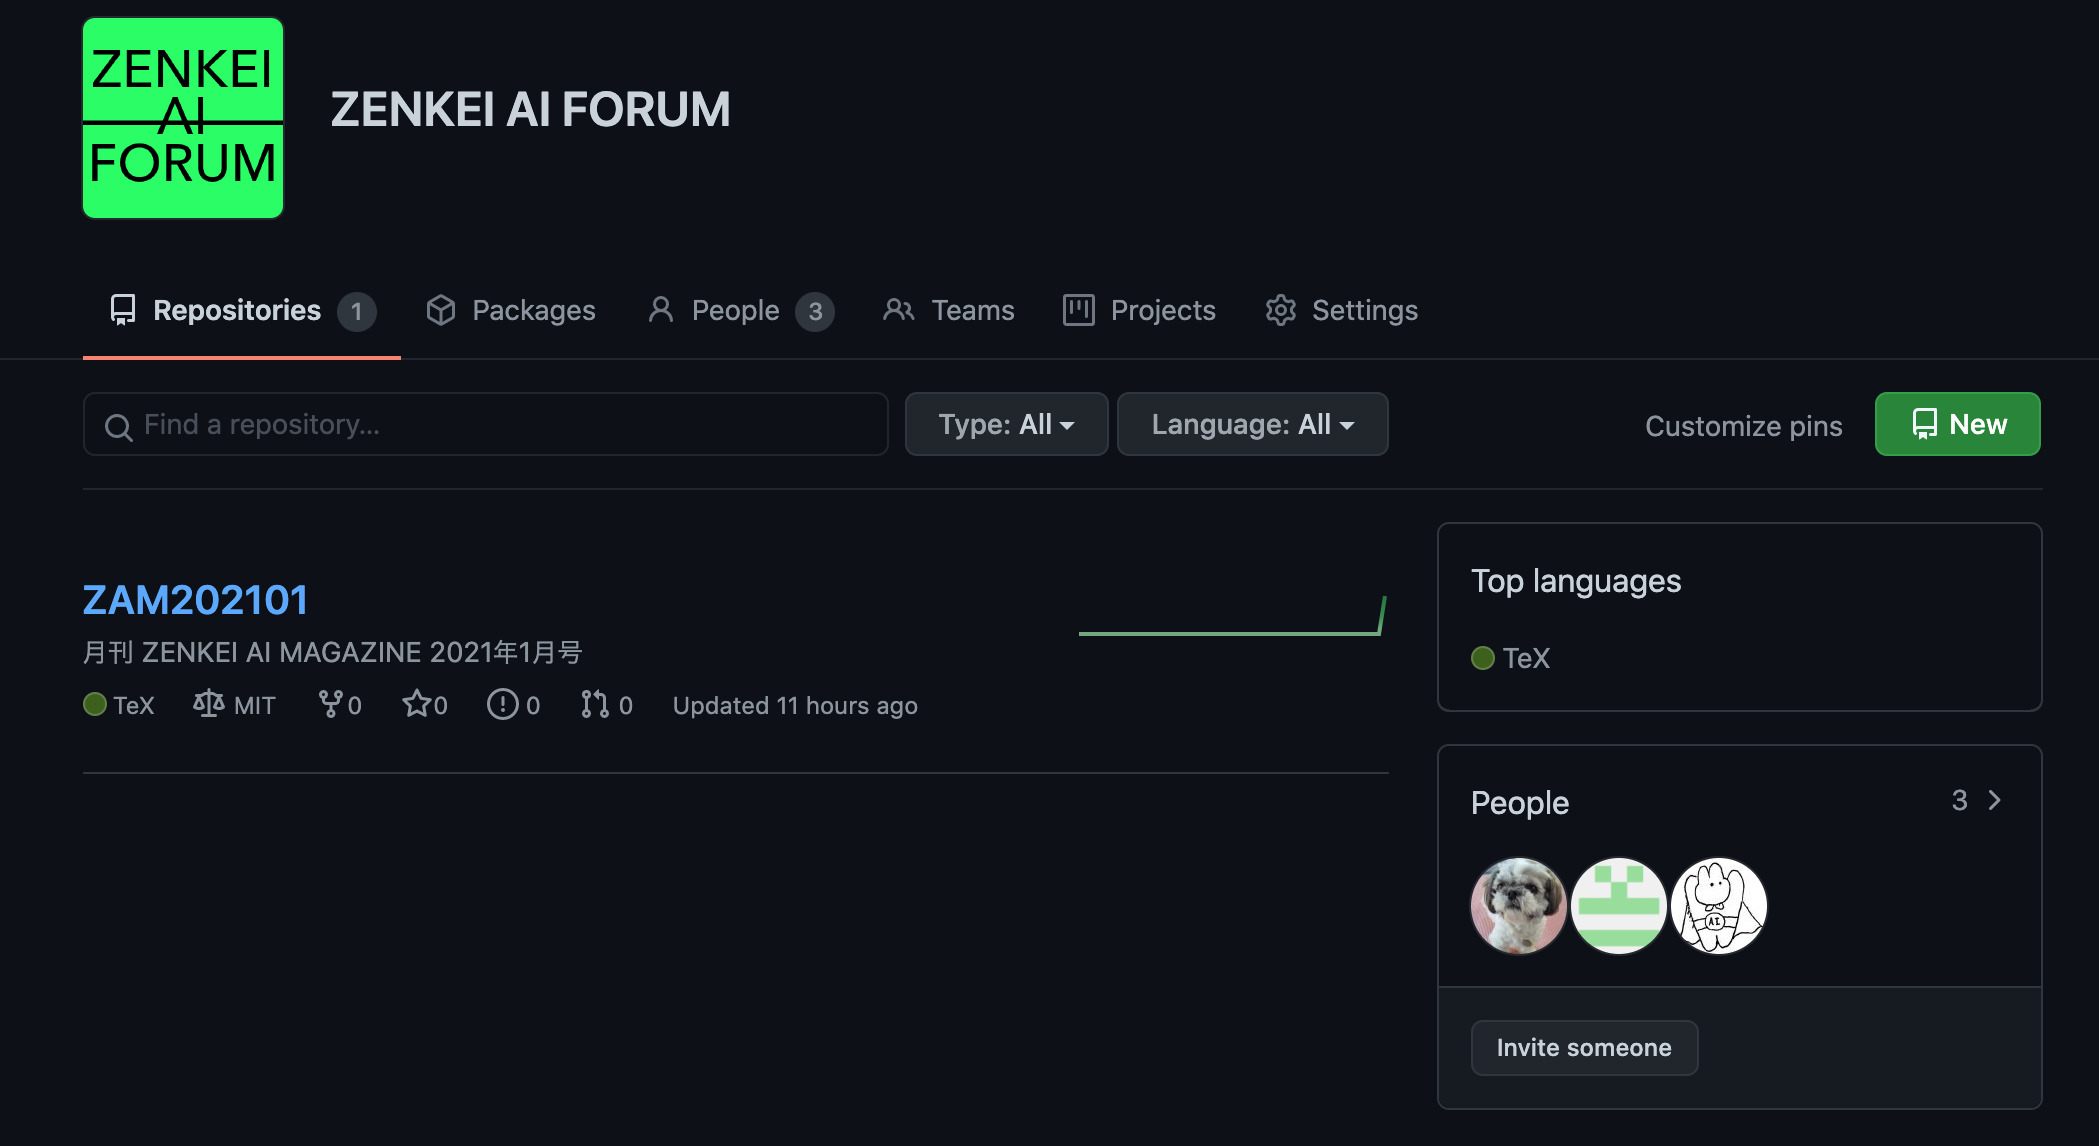
\includegraphics[width=0.63\textwidth]
      {images/github-01.jpg}
  };  
\end{tikzpicture}

\vspace{5.0cm}

ということで、まず \texttt{zenkei-ai-forum} という組織アカウント
(GitHub の用語でいう ``organization'')を作り、
そこに \texttt{ZAM202101} というレポジトリ
(\url{https://github.com/zenkei-ai-forum/ZAM202101})
を作りました。

\begin{tikzpicture}[remember picture, overlay]
  \node[xshift=4.6cm,yshift=5.5cm] at (current page.center){
    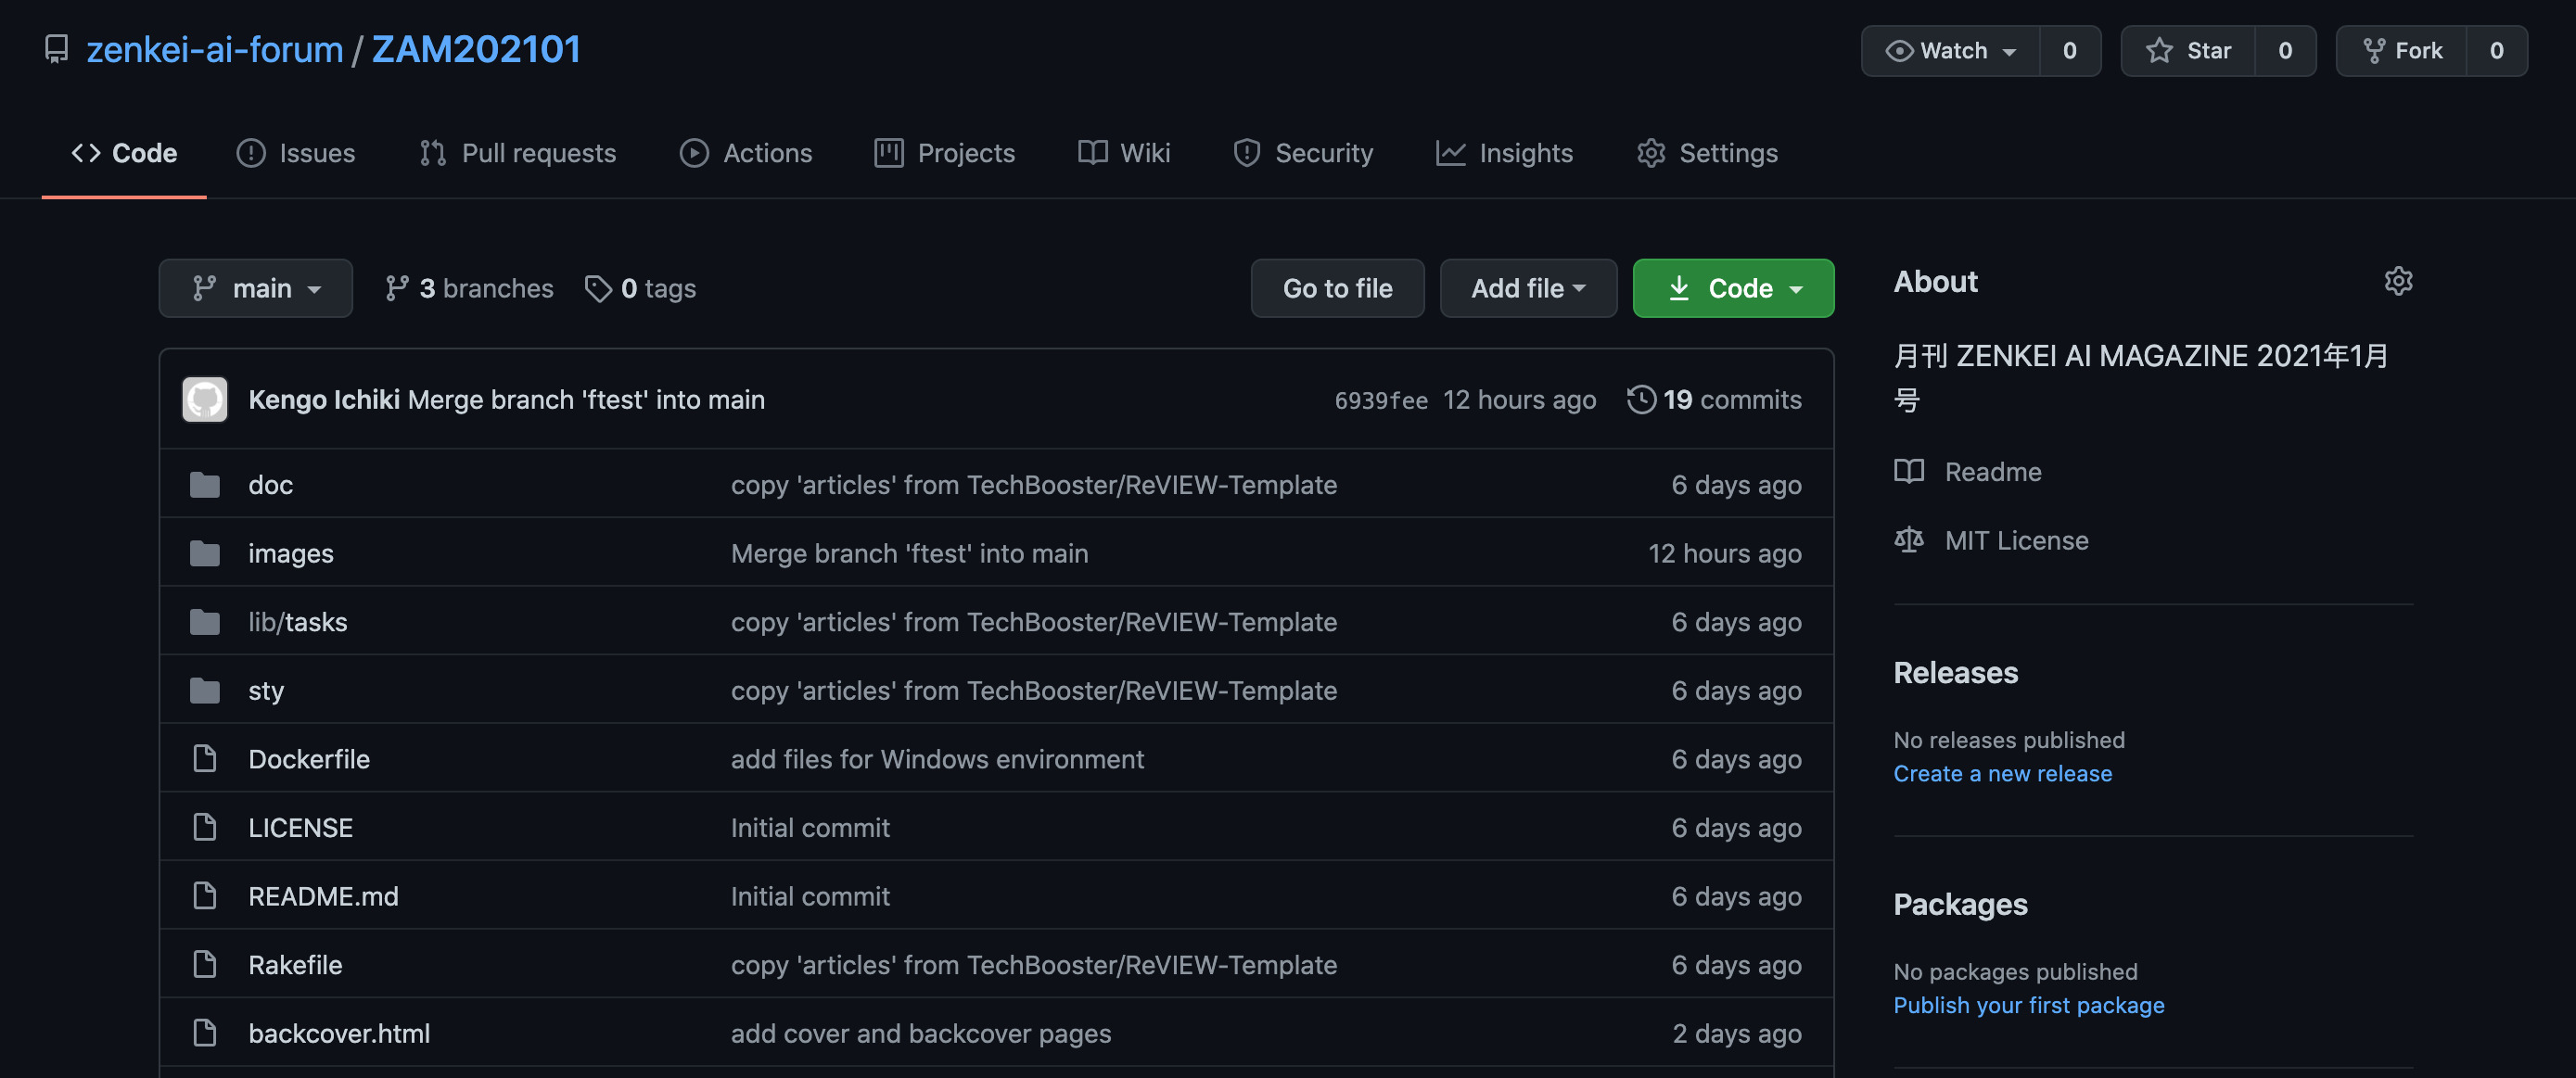
\includegraphics[width=0.63\textwidth]
      {images/github-02.jpg}
  };  
\end{tikzpicture}

\vspace{3.5cm}

このレポジトリをプログラム開発よろしく、各人が自分のコンピュータに
clone して加筆して commit して push して、
他のメンバーが pull して加筆して commit して push して、と。
なんか AI FORUM って感じですね。

\begin{tikzpicture}[remember picture, overlay]
  \node[xshift=4.6cm,yshift=-3.0cm] at (current page.center){
    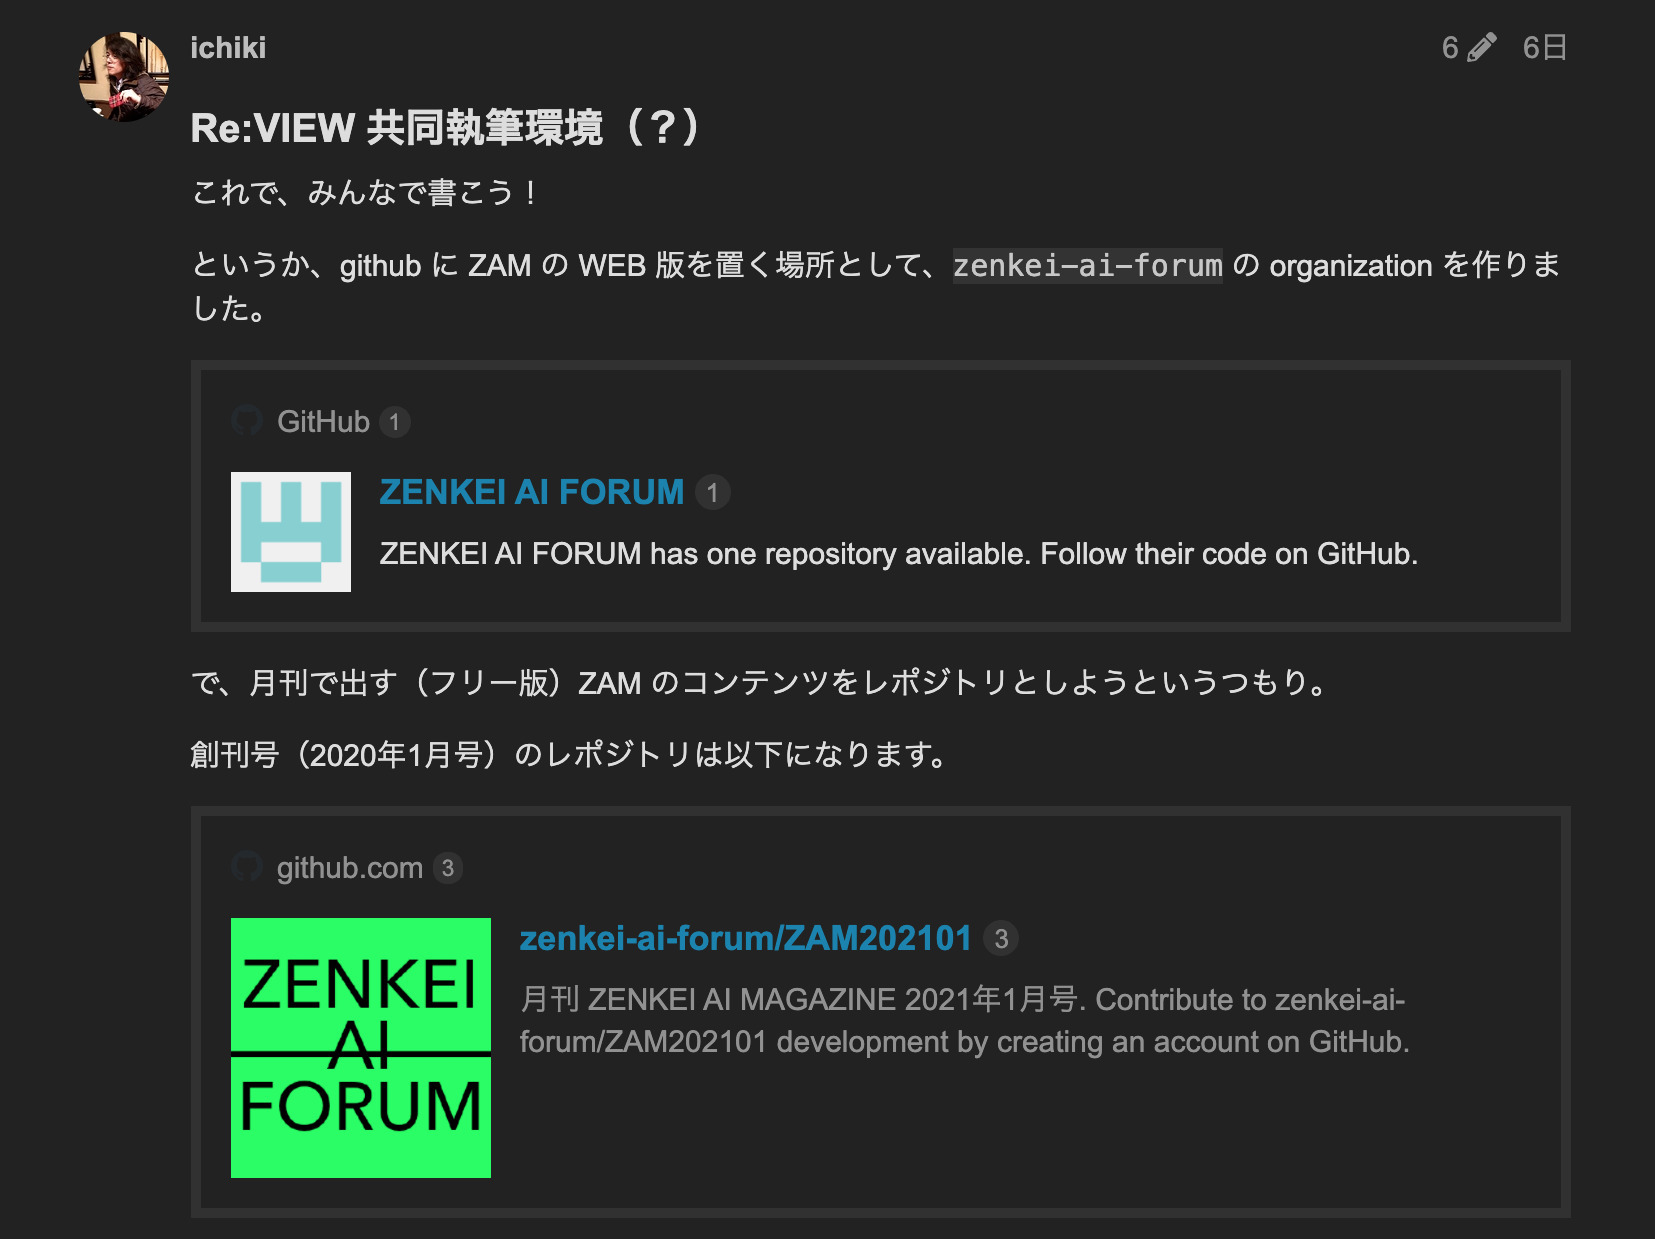
\includegraphics[width=0.63\textwidth]
      {images/online-forum-03.jpg}
  };  
\end{tikzpicture}

\vspace{7.0cm}

環境が整ったので、今回の執筆メンバーに声掛けして、実際に創刊号の執筆が始まりました。
実際の(共同)執筆は順調に進んだか、と言うと必ずしもそうではなかったです。
わたし自身が感じたことは Re:VIEW の表現力が限定的であること
(ここでの比較の対象は \LaTeX{} になりますが)。
実績として沢山の技術系同人誌の執筆に使われていて、
「本」「単行本」という形式(文字がメインのコンテンツ)においては
必要十分だと思いますが、
今回わたしたちが作っている『月刊 ZAM』は「雑誌」です。
雑誌といえば、カラフルな写真やイラストが誌面にあふれ、
デザインもバリエーションがあります。
それがあんまりできそうにない。
この辺のことは、上にも書いた共同執筆という状況と、
創刊号はまず出すことが大事ということで、この縛りの中でがんばることにします。
共同執筆に関しては、基本的に各人が担当の章を書くという形だったので、
原稿の投稿が GitHub への push になった(だけ)でした。

\begin{tikzpicture}[remember picture, overlay]
  \node[xshift=-4.6cm,yshift=-3.2cm] at (current page.center){
    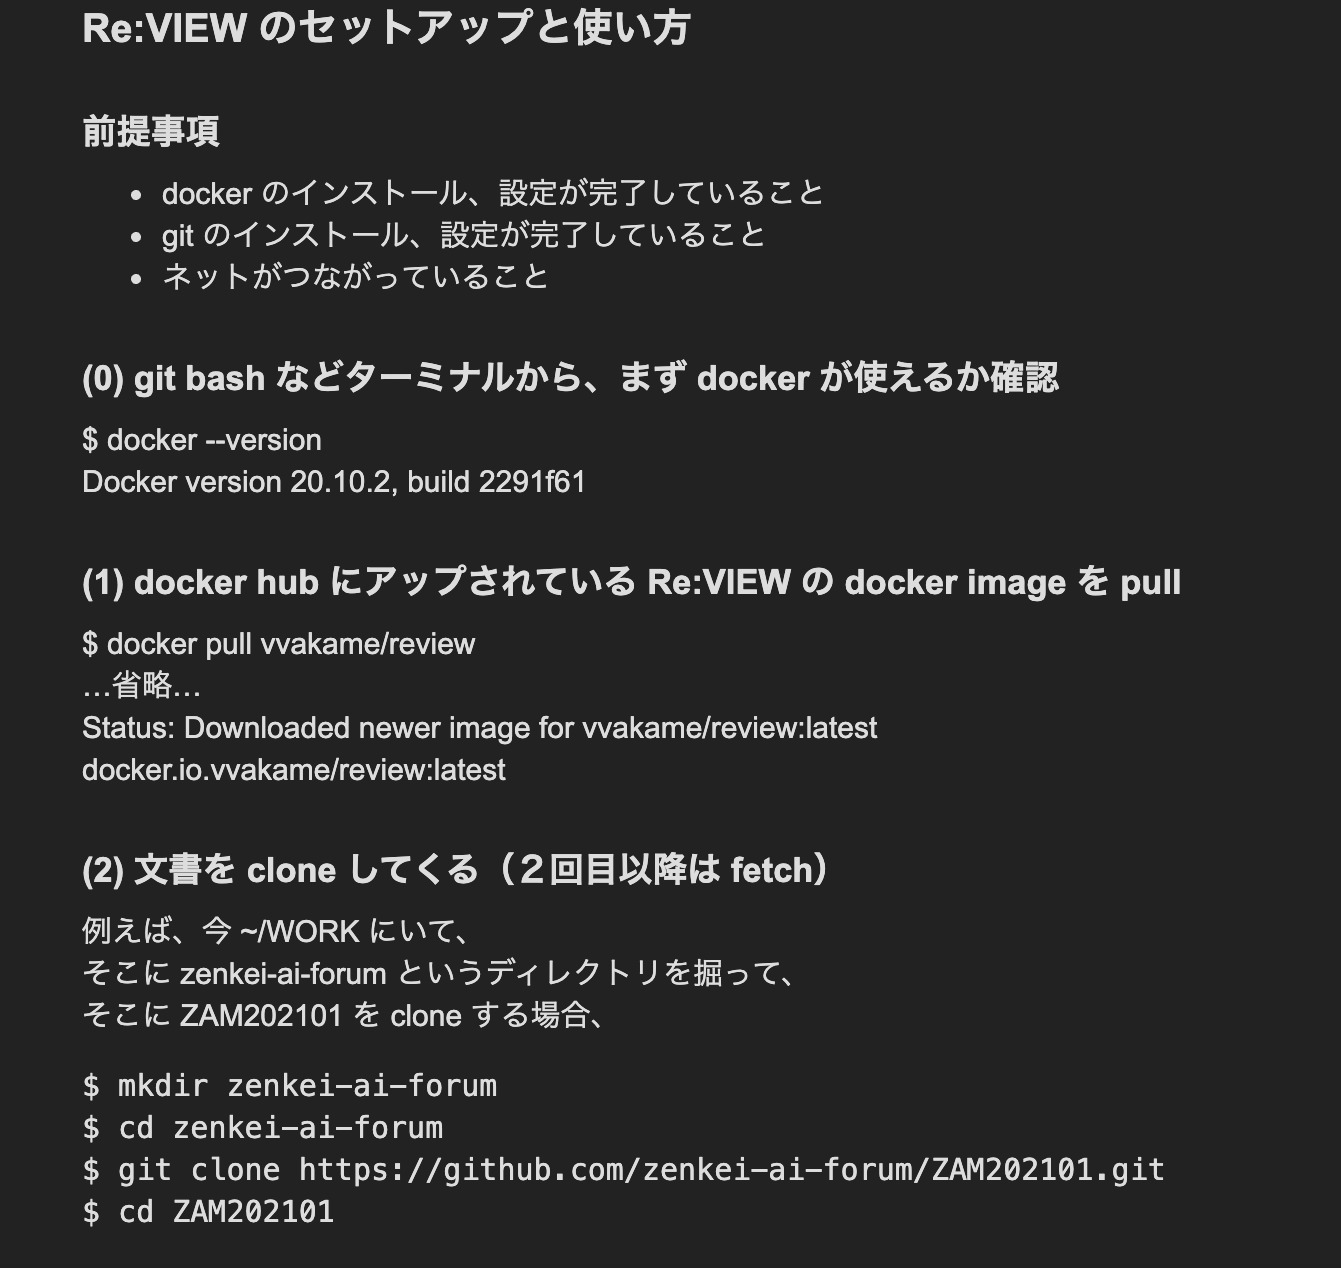
\includegraphics[width=0.63\textwidth]
      {images/online-forum-04.jpg}
  };  
\end{tikzpicture}

%\vspace{7.0cm}
\vspace{5.0cm}

\begin{tikzpicture}[remember picture, overlay]
  \node[xshift=-4.605cm,yshift=-10.15cm] at (current page.center){
    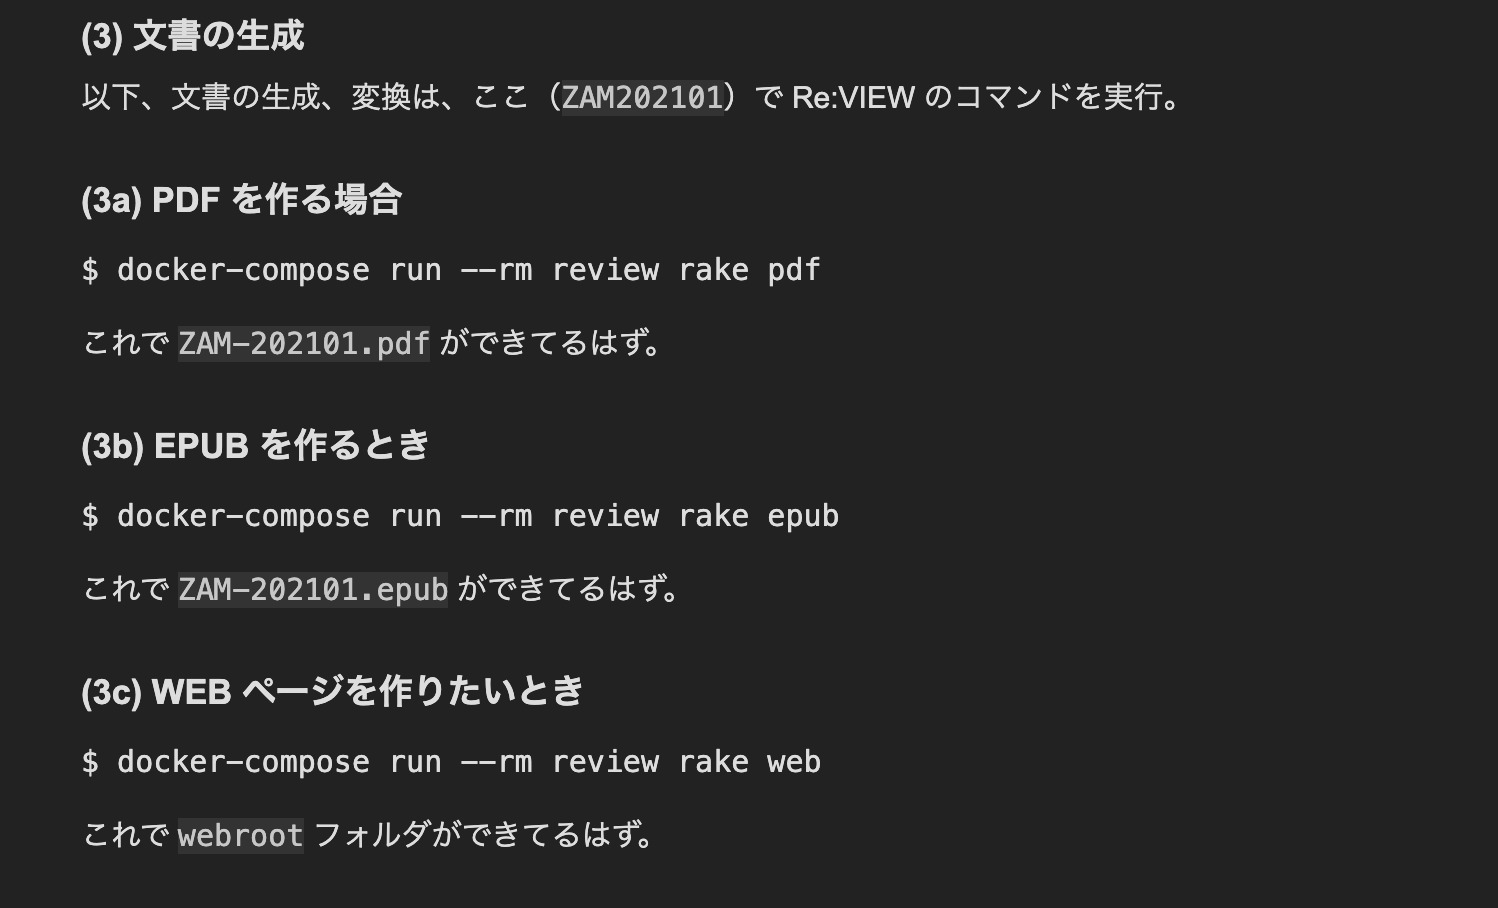
\includegraphics[width=0.63\textwidth]
      {images/online-forum-05.jpg}
  };  
\end{tikzpicture}

\vspace{7.0cm}

 % 全角スペース

\begin{tikzpicture}[remember picture, overlay]
  \node[xshift=4.6cm,yshift=5.5cm] at (current page.center){
    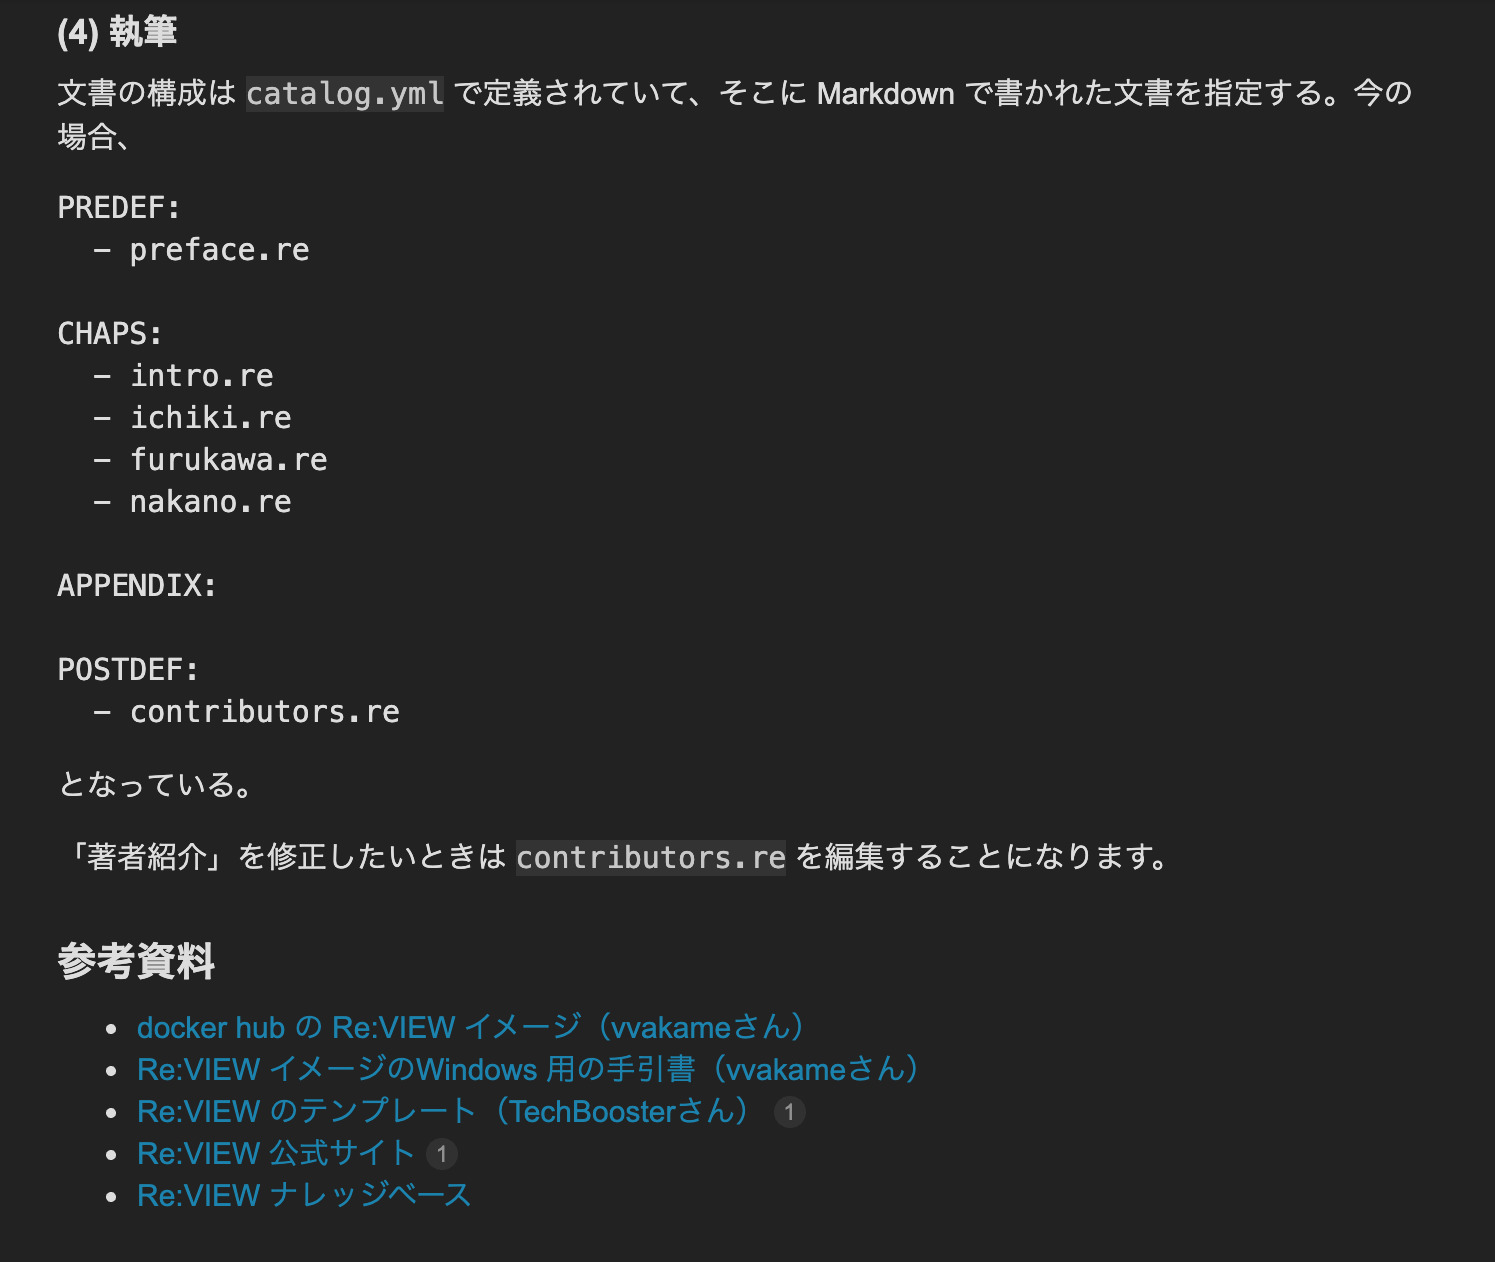
\includegraphics[width=0.63\textwidth]
      {images/online-forum-06.jpg}
  };  
\end{tikzpicture}

\vspace{7.0cm}

環境設定から執筆までの簡単な手引きをオンラインフォーラムに投稿しました。
興味ある方はご自身のコンピュータにセットアップして、
\texttt{ZAM202101} レポジトリ
(\url{https://github.com/zenkei-ai-forum/ZAM202101})
を clone して、手元でビルドしてみてはどうでしょうか。


\section{創刊号、完成!}
今回の執筆陣は(わたしを除いて)きちんとスケジュール管理ができる
『技術書典』を潜り抜けてきた人たちなので、
予定通り 2 月の ZAF に無事、記念すべき創刊号である
オンライン版『月刊 ZAM 2021年1月号』発行となりました!
(つまり、わたしの原稿が一番遅かった、ということです。
でも、雑誌創刊にあたり書き下ろす「巻頭言」とか、
表紙のデザインとか、いろいろとあったんですよ。)

Re:VIEW の利点として、1つのソースで複数のフォーマットに出力できる
ということがあります。
(電子)書籍の執筆においてはやはり PDF がメインになると思いますが、
web 版、 epub 版もコマンド一発で出力できます(基本的には)。
ただし、やはり細かいデザインとか気になる部分が出てきます
(表紙ページ、裏表紙ページの扱いや、目次、ページ遷移のリンクなど)。
今回は一度出力された HTML を手で修正して最終版としました。

『月刊 ZAM 2021年1月号』 web 版のリンクは
\url{https://zenkei-ai-forum.github.io/ZAM202101/}
PDF 版は \url{https://zenkei-ai-forum.github.io/ZAM202101/ZAM202101-v2.pdf}
になります。

\end{multicols}

\hrule

\begin{tikzpicture}[remember picture, overlay]
  \node[xshift=-7.4cm,yshift=3.5cm] at (current page.center){
    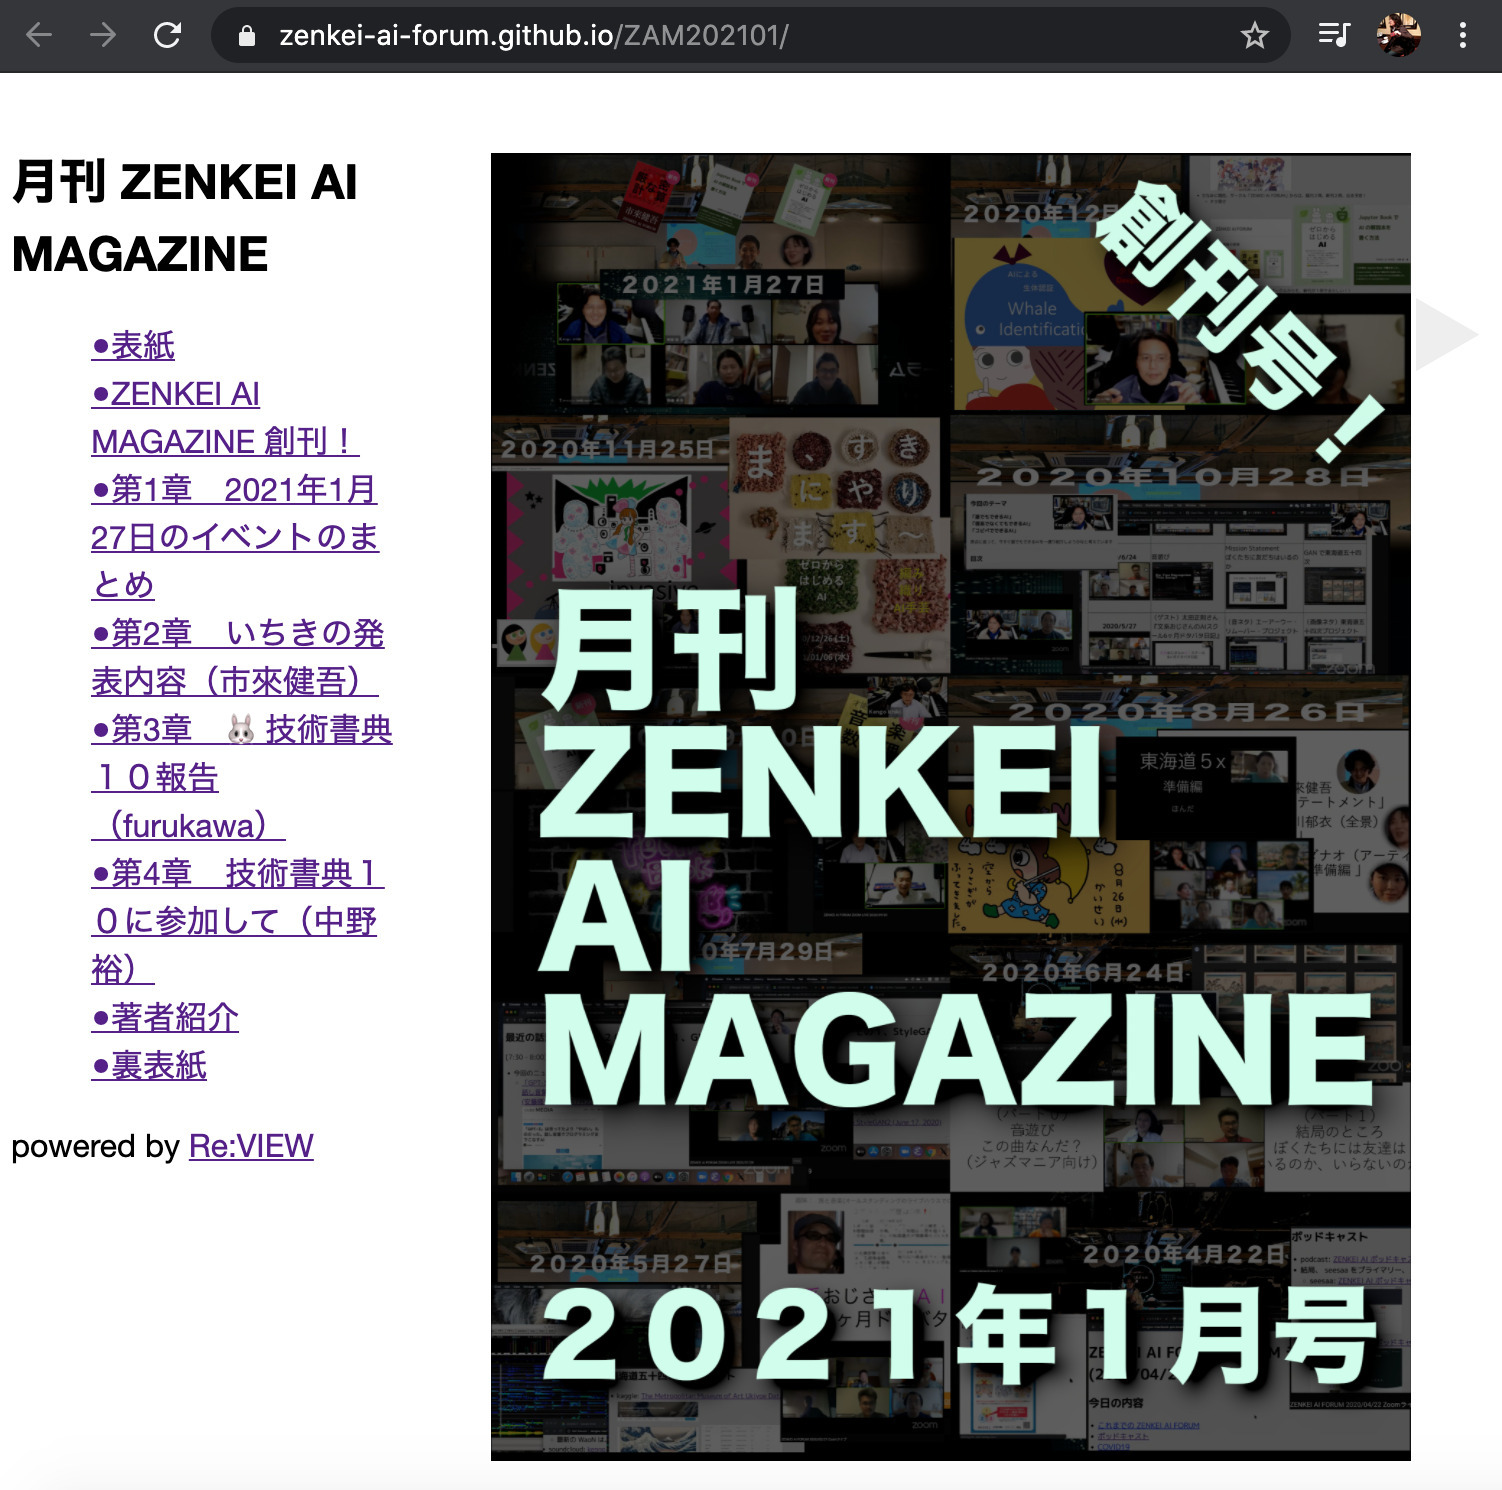
\includegraphics[height=0.18\textheight]
      {images/ZAM202101-web-01.jpg}
  };  
\end{tikzpicture}
\begin{tikzpicture}[remember picture, overlay]
  \node[xshift=-3.7cm,yshift=3.5cm] at (current page.center){
    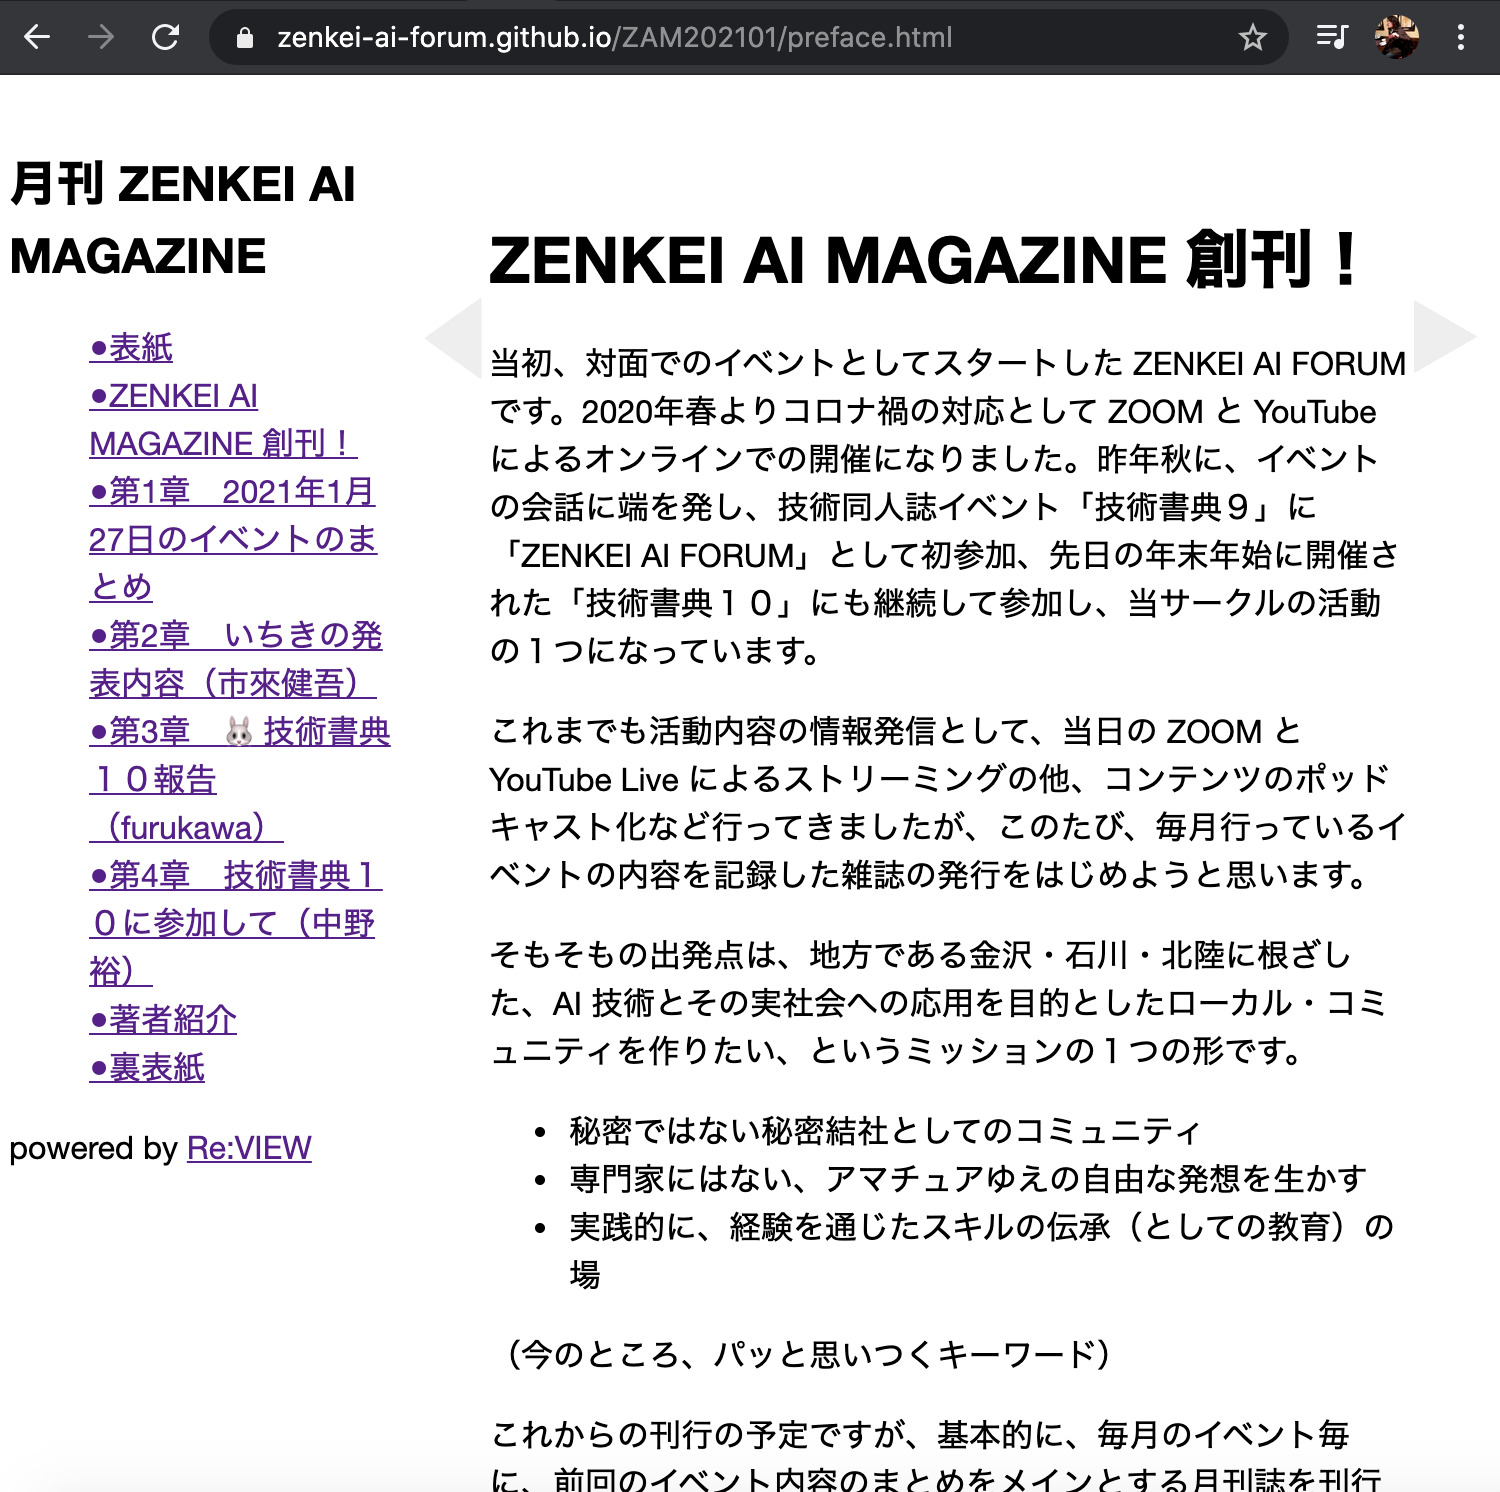
\includegraphics[height=0.18\textheight]
      {images/ZAM202101-web-02.jpg}
  };  
\end{tikzpicture}
\begin{tikzpicture}[remember picture, overlay]
  \node[xshift=0.0cm,yshift=3.5cm] at (current page.center){
    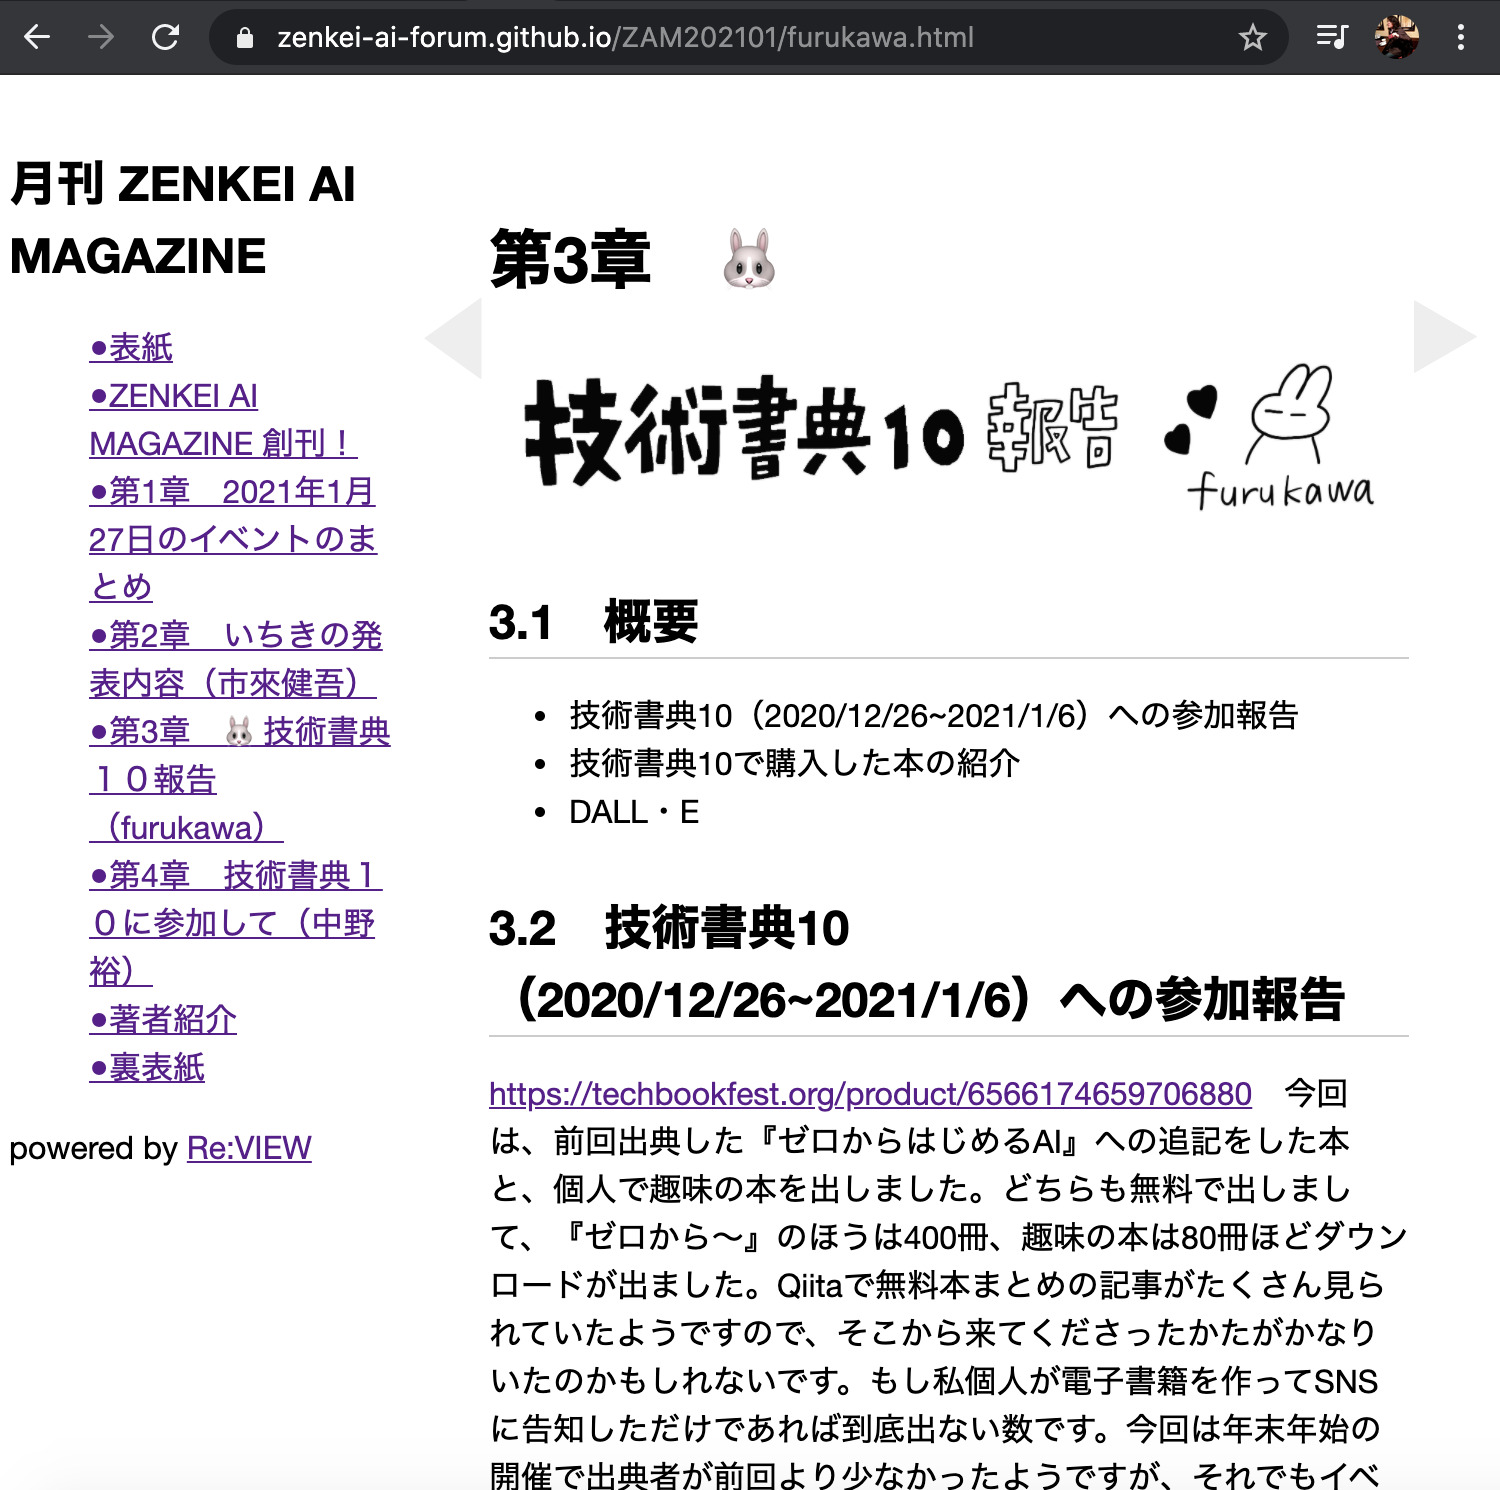
\includegraphics[height=0.18\textheight]
      {images/ZAM202101-web-03.jpg}
  };  
\end{tikzpicture}
\begin{tikzpicture}[remember picture, overlay]
  \node[xshift=3.7cm,yshift=3.5cm] at (current page.center){
    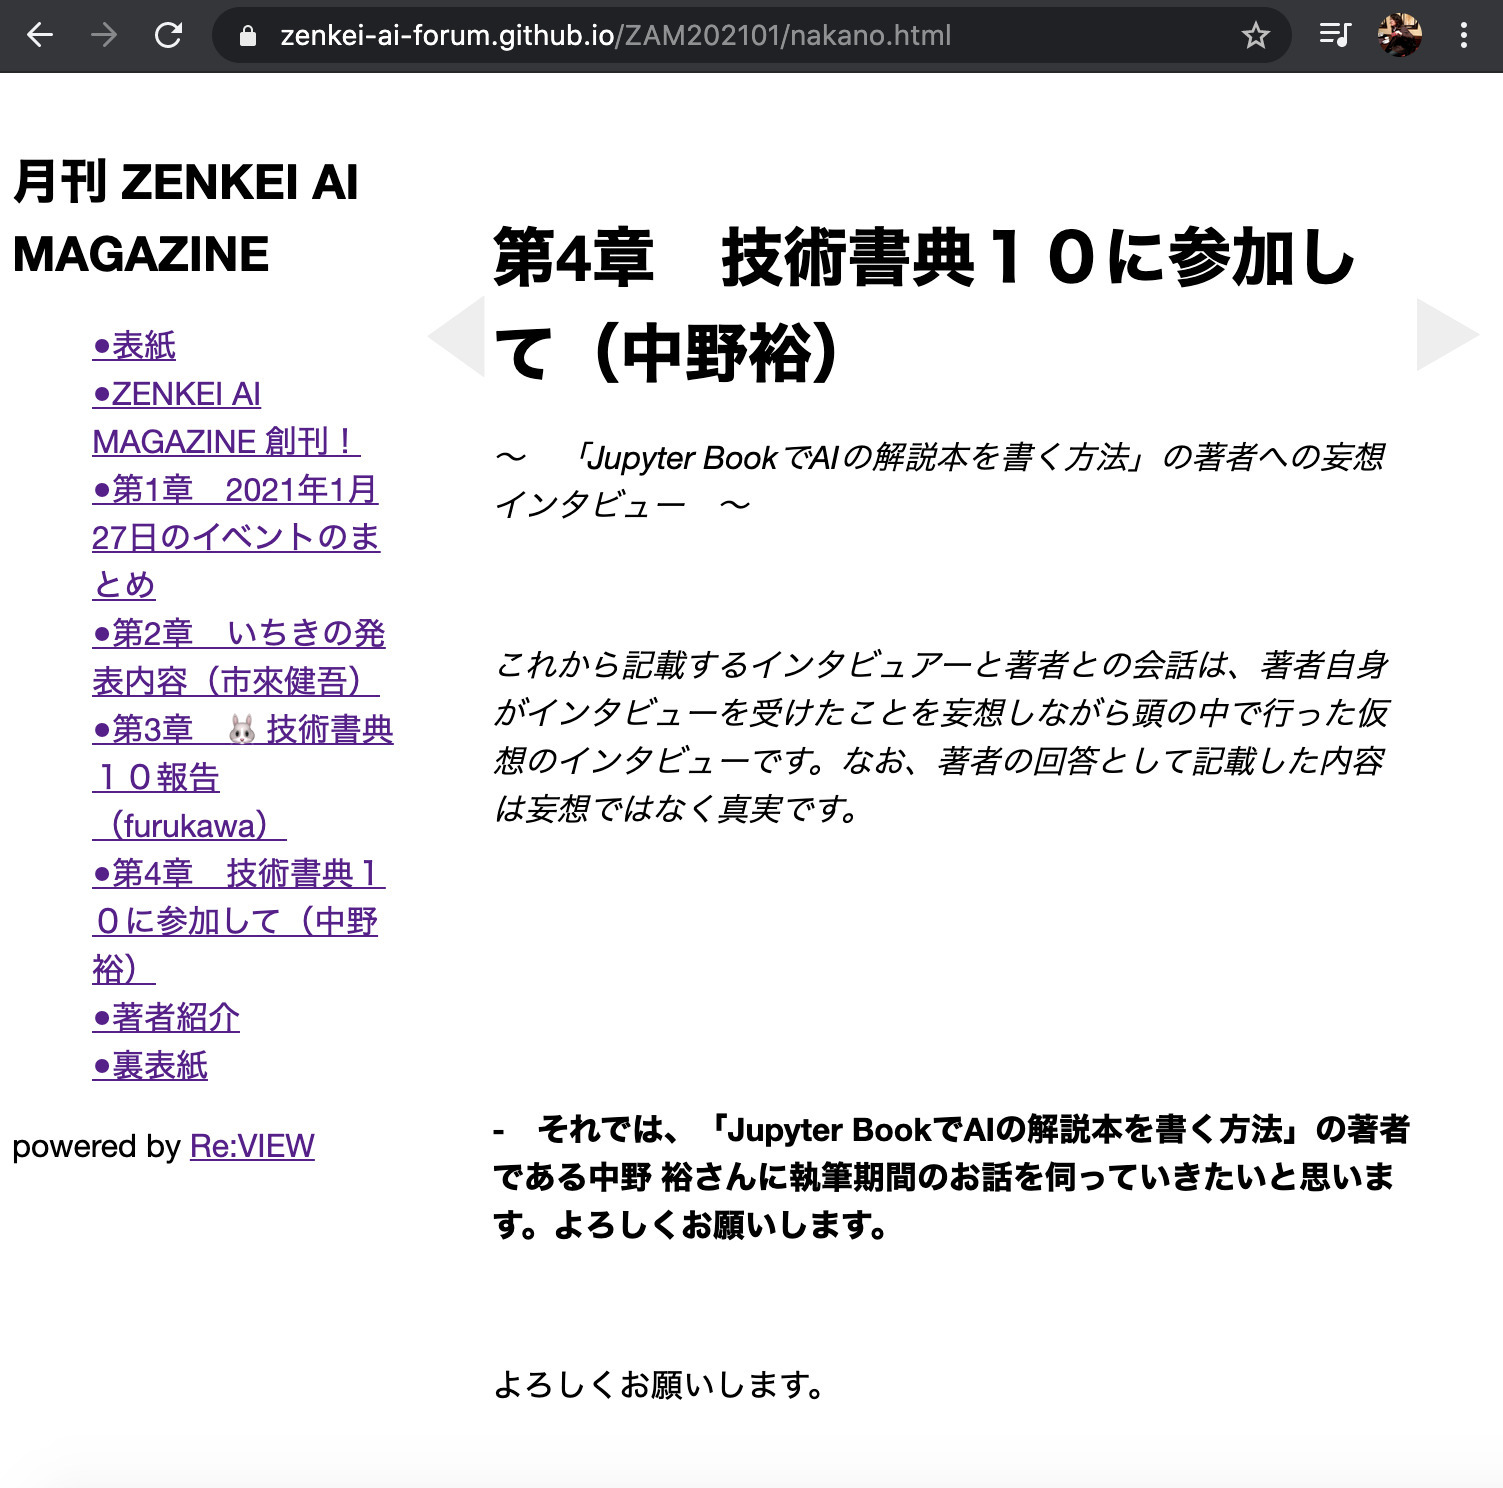
\includegraphics[height=0.18\textheight]
      {images/ZAM202101-web-04.jpg}
  };  
\end{tikzpicture}
\begin{tikzpicture}[remember picture, overlay]
  \node[xshift=7.4cm,yshift=3.5cm] at (current page.center){
    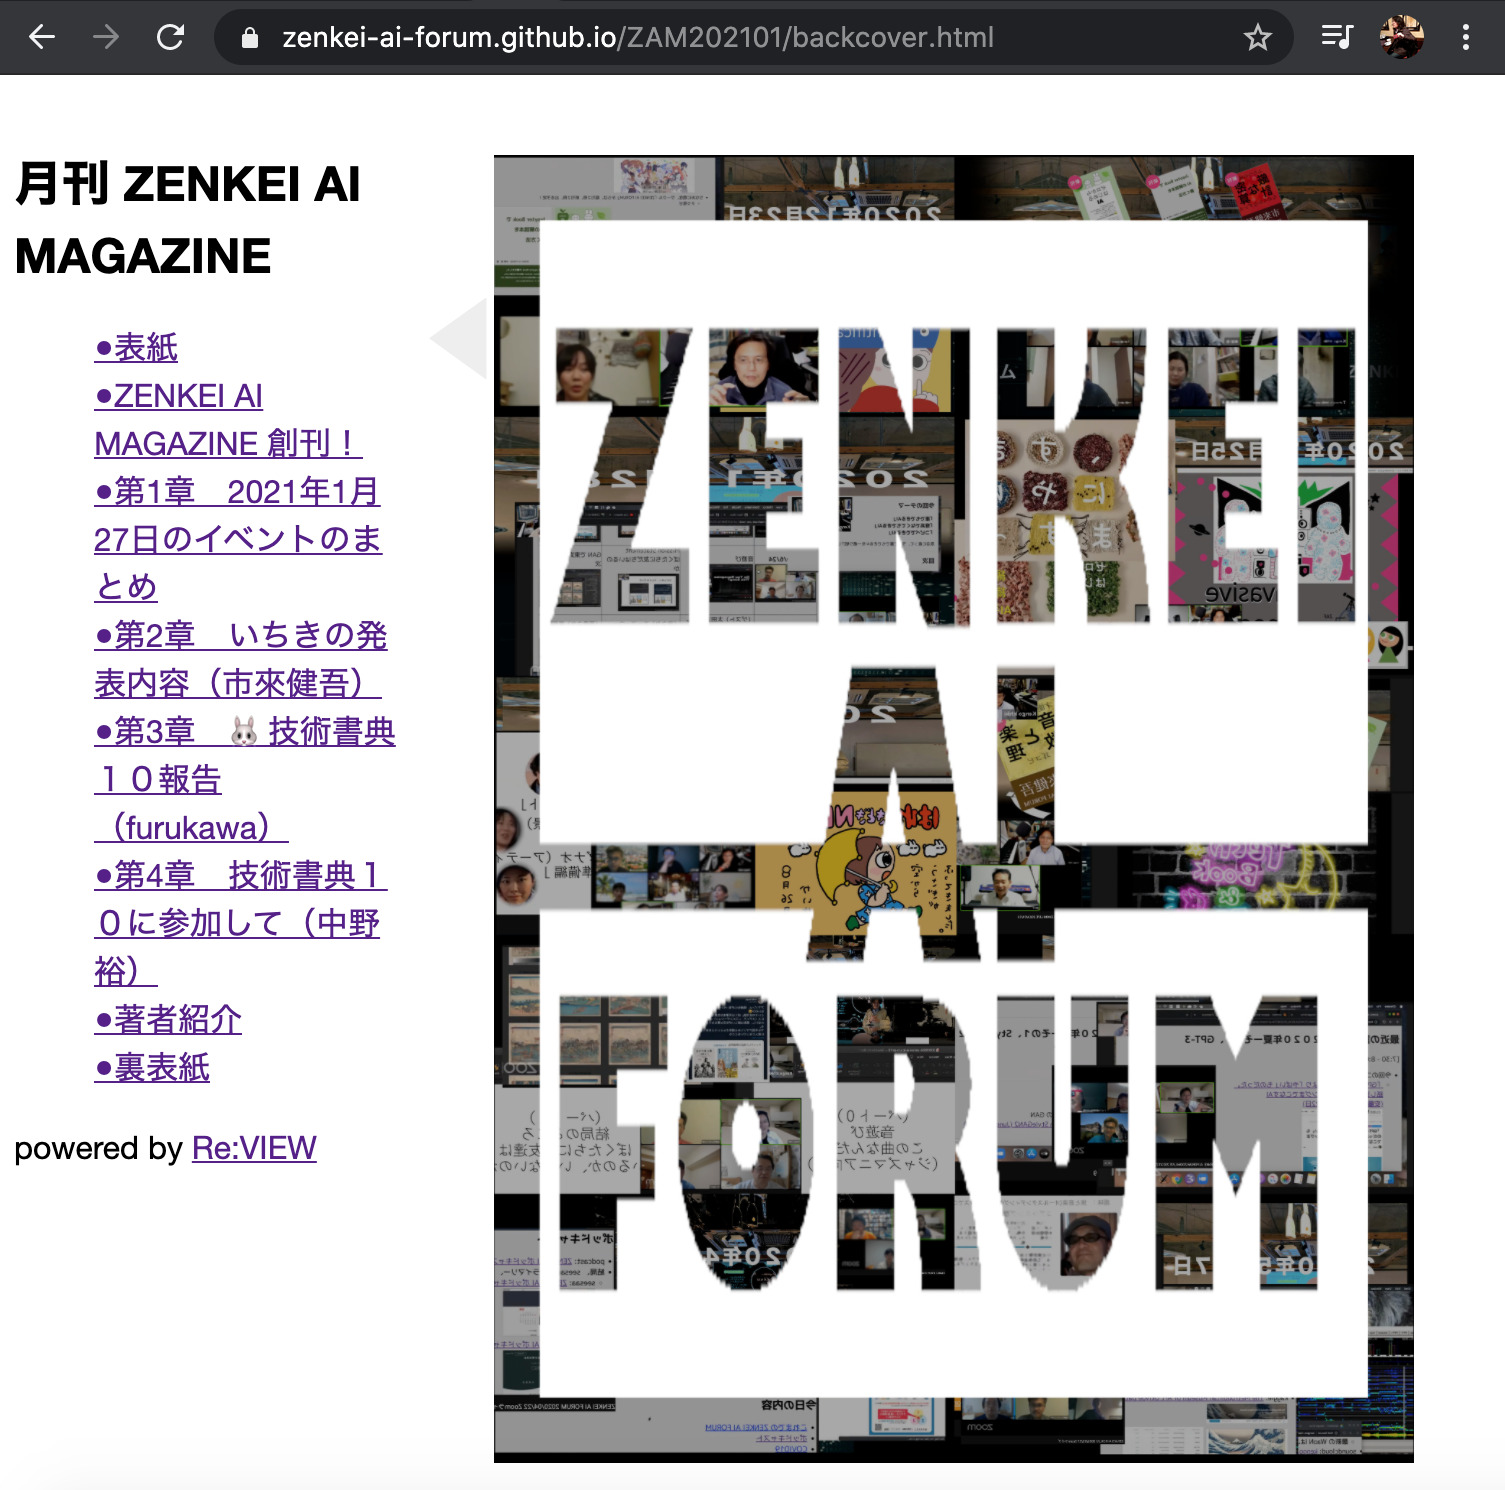
\includegraphics[height=0.18\textheight]
      {images/ZAM202101-web-05.jpg}
  };  
\end{tikzpicture}

\vspace{0.175\textheight}

\begin{center}
  web 版『月刊 ZAM』創刊号のスクショ
\end{center}

\begin{tikzpicture}[remember picture, overlay]
  \node[xshift=-7.4cm,yshift=-1.5cm] at (current page.center){
    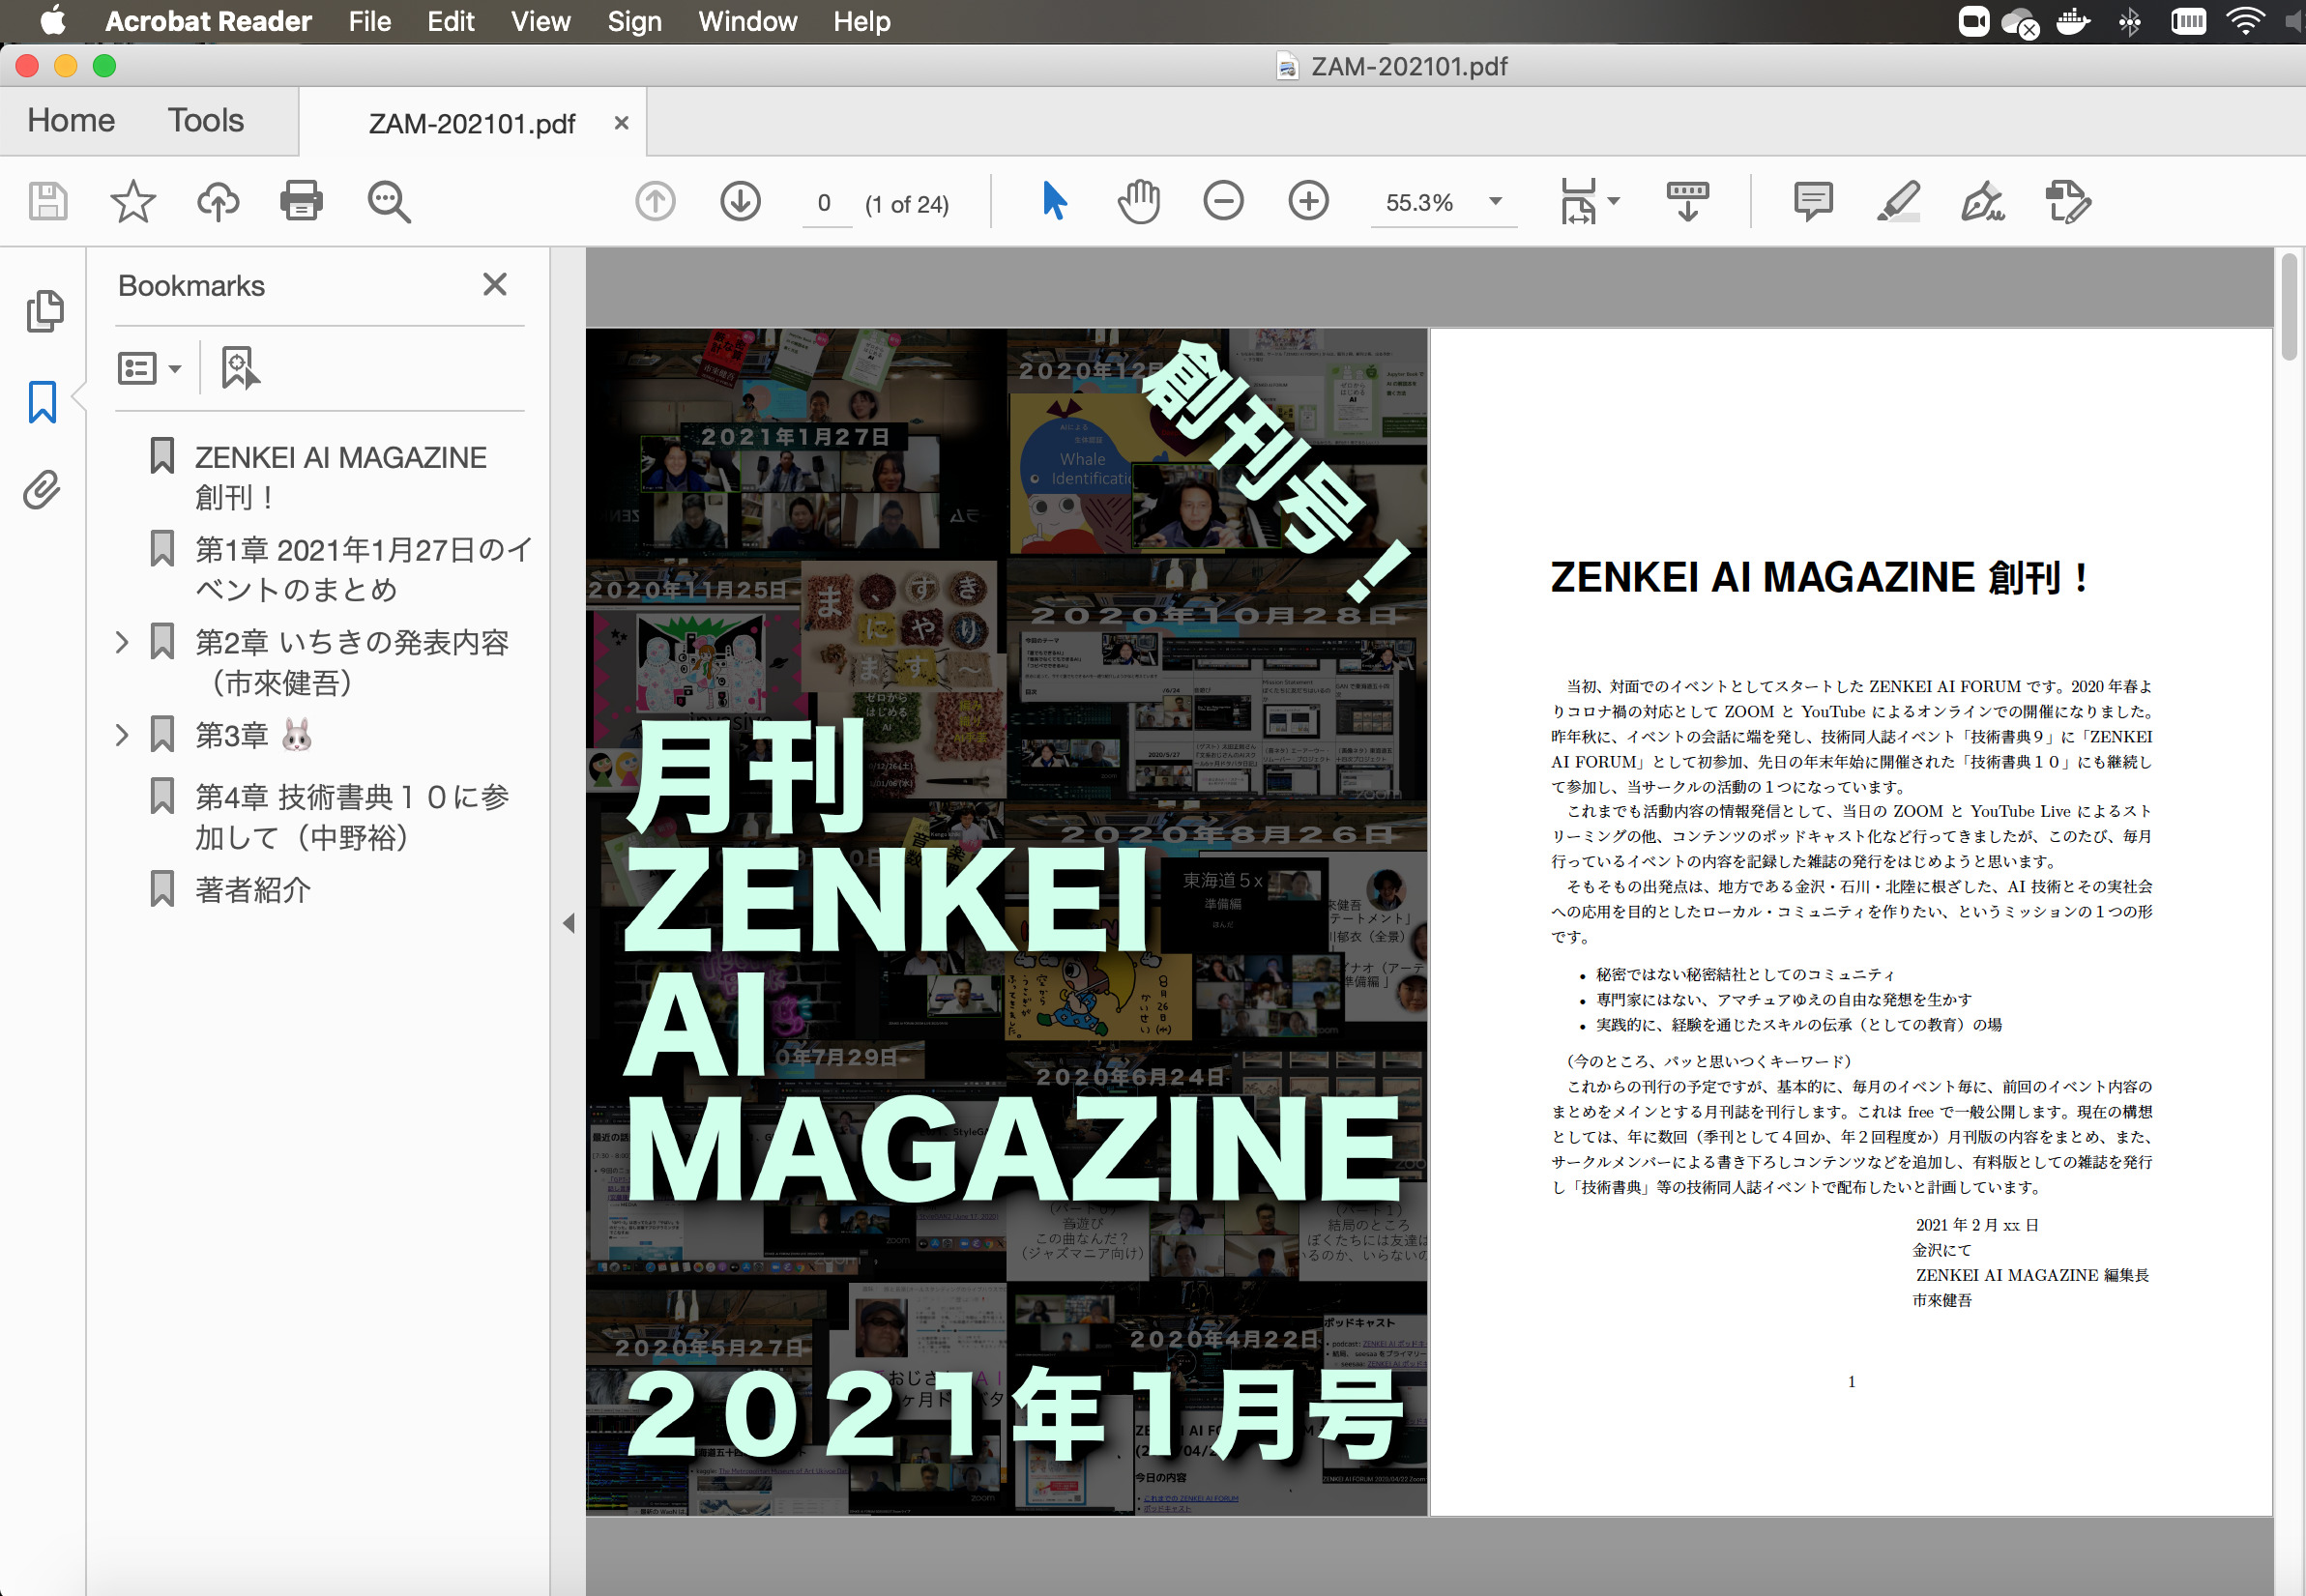
\includegraphics[height=0.18\textheight]
      {images/ZAM202101-pdf-01.jpg}
  };  
\end{tikzpicture}
\begin{tikzpicture}[remember picture, overlay]
  \node[xshift=-2.5cm,yshift=-1.5cm] at (current page.center){
    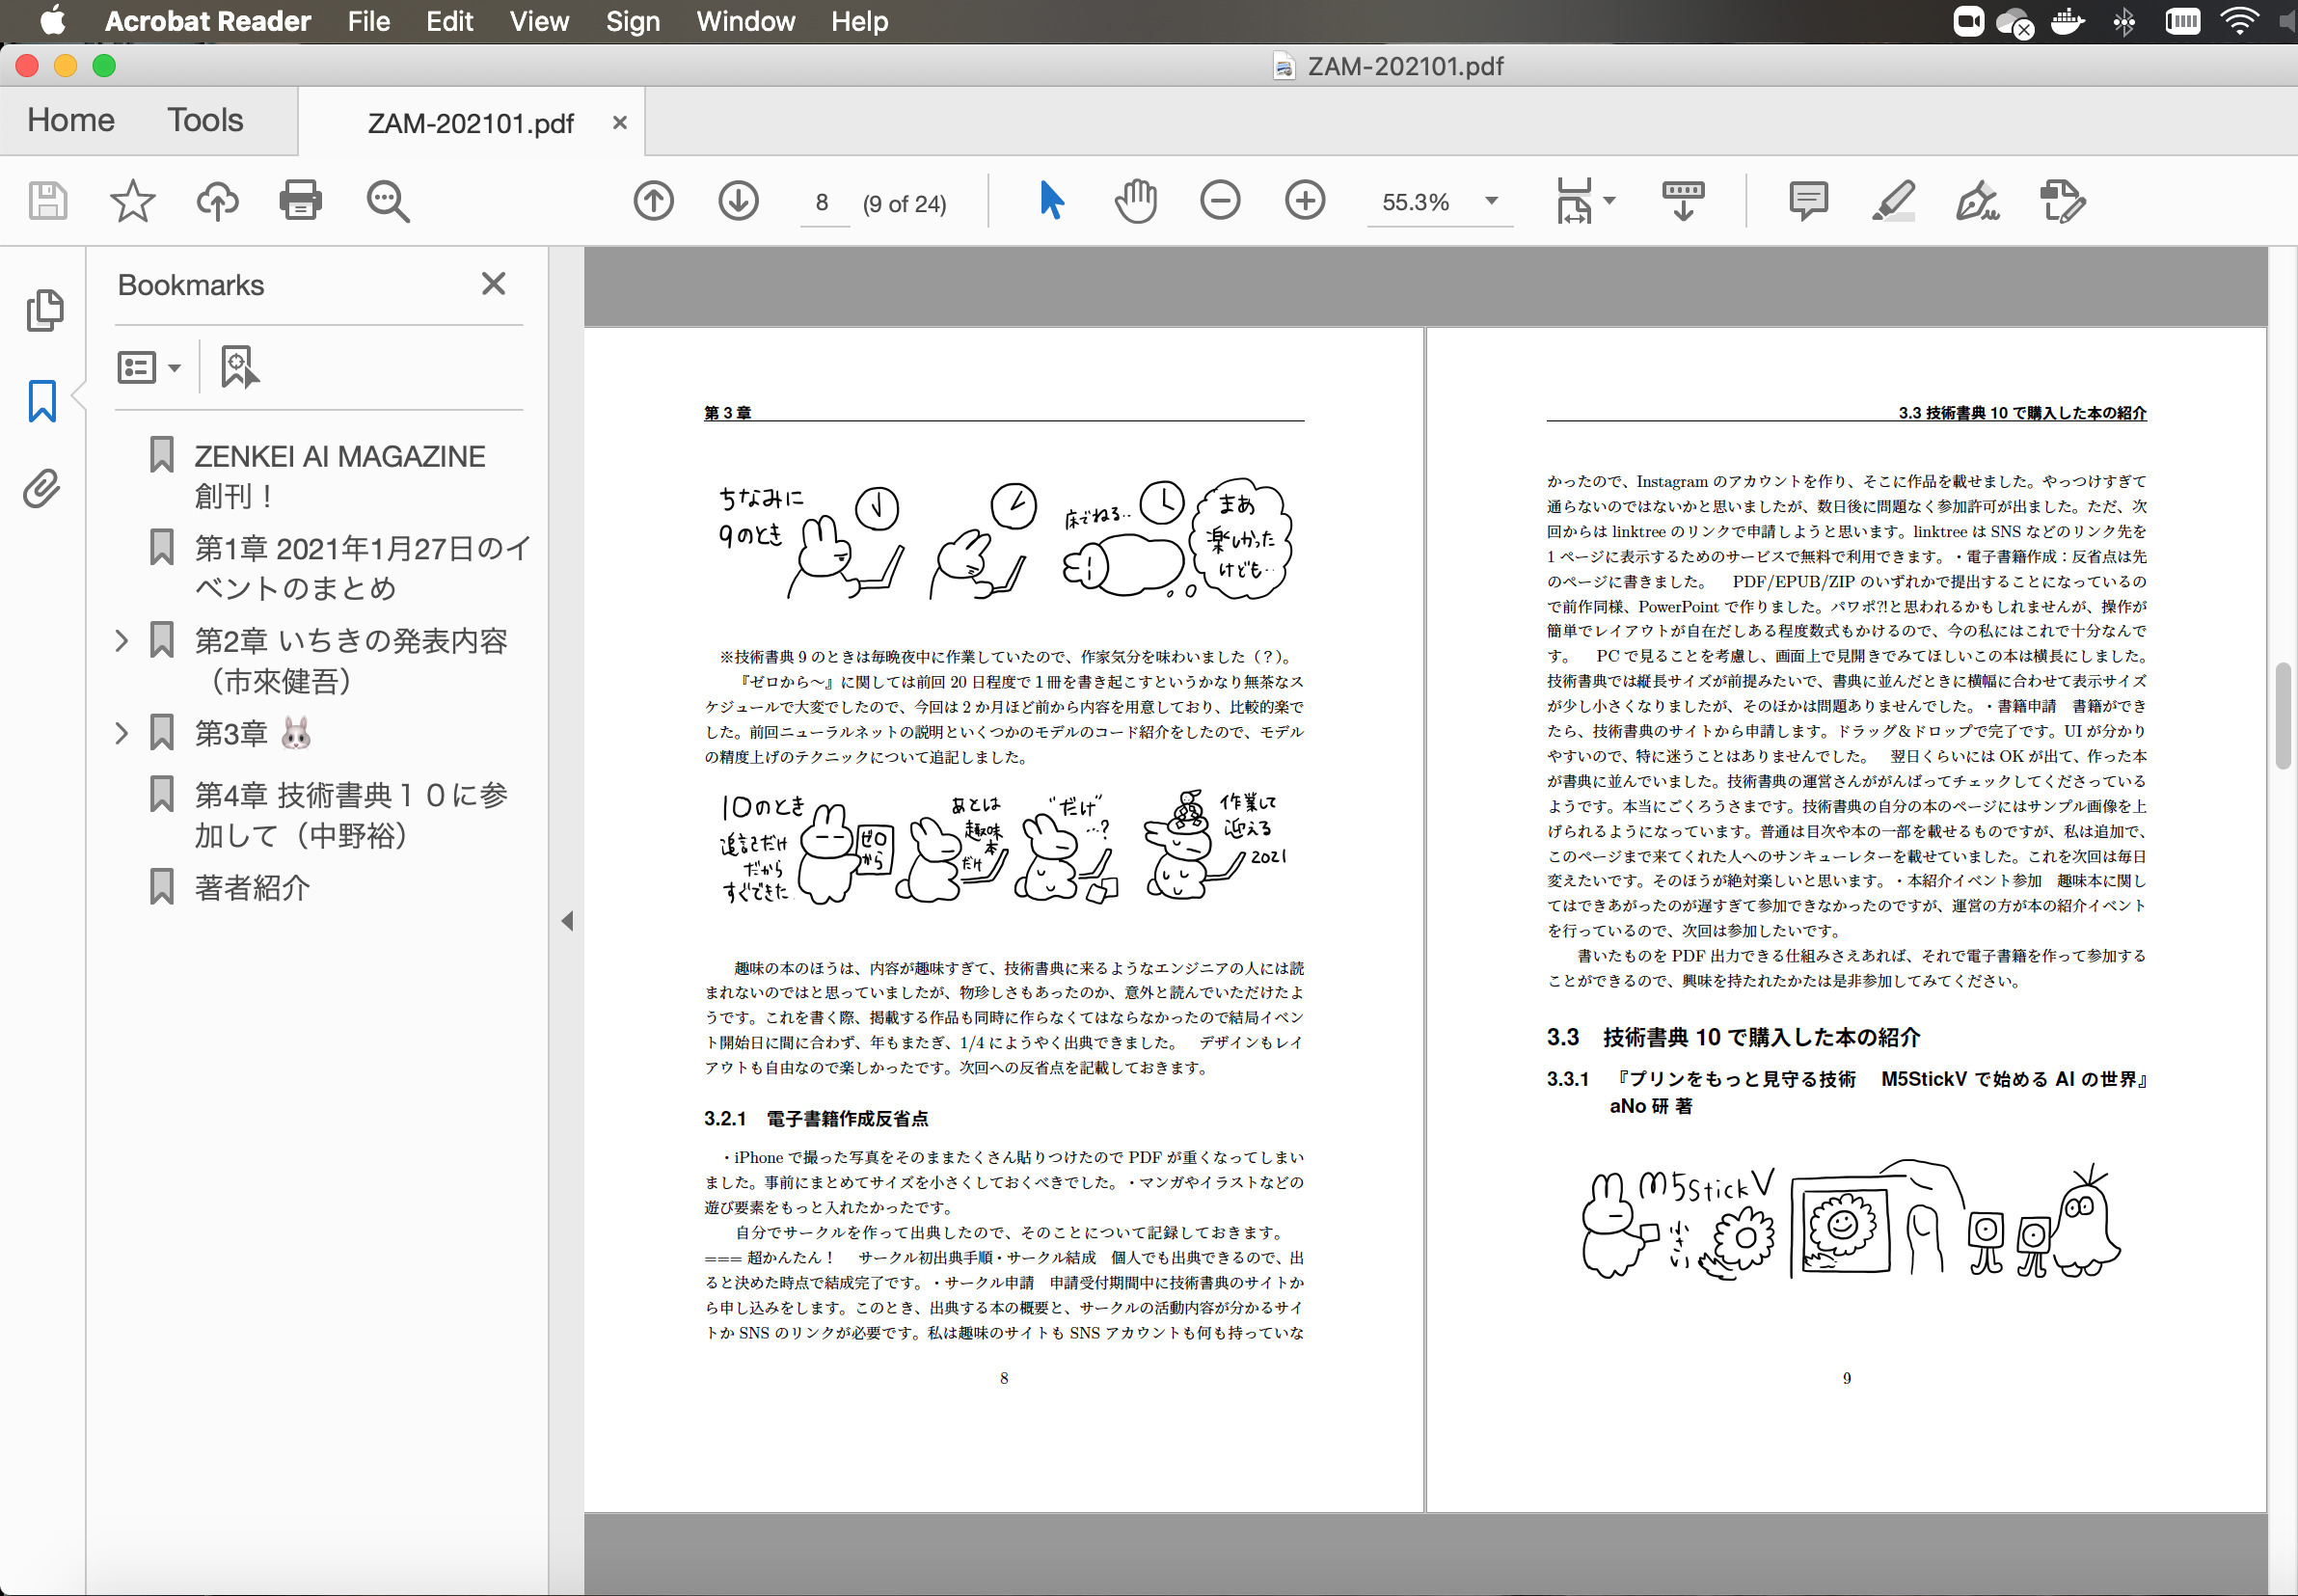
\includegraphics[height=0.18\textheight]
      {images/ZAM202101-pdf-02.jpg}
  };  
\end{tikzpicture}
\begin{tikzpicture}[remember picture, overlay]
  \node[xshift=2.5cm,yshift=-1.5cm] at (current page.center){
    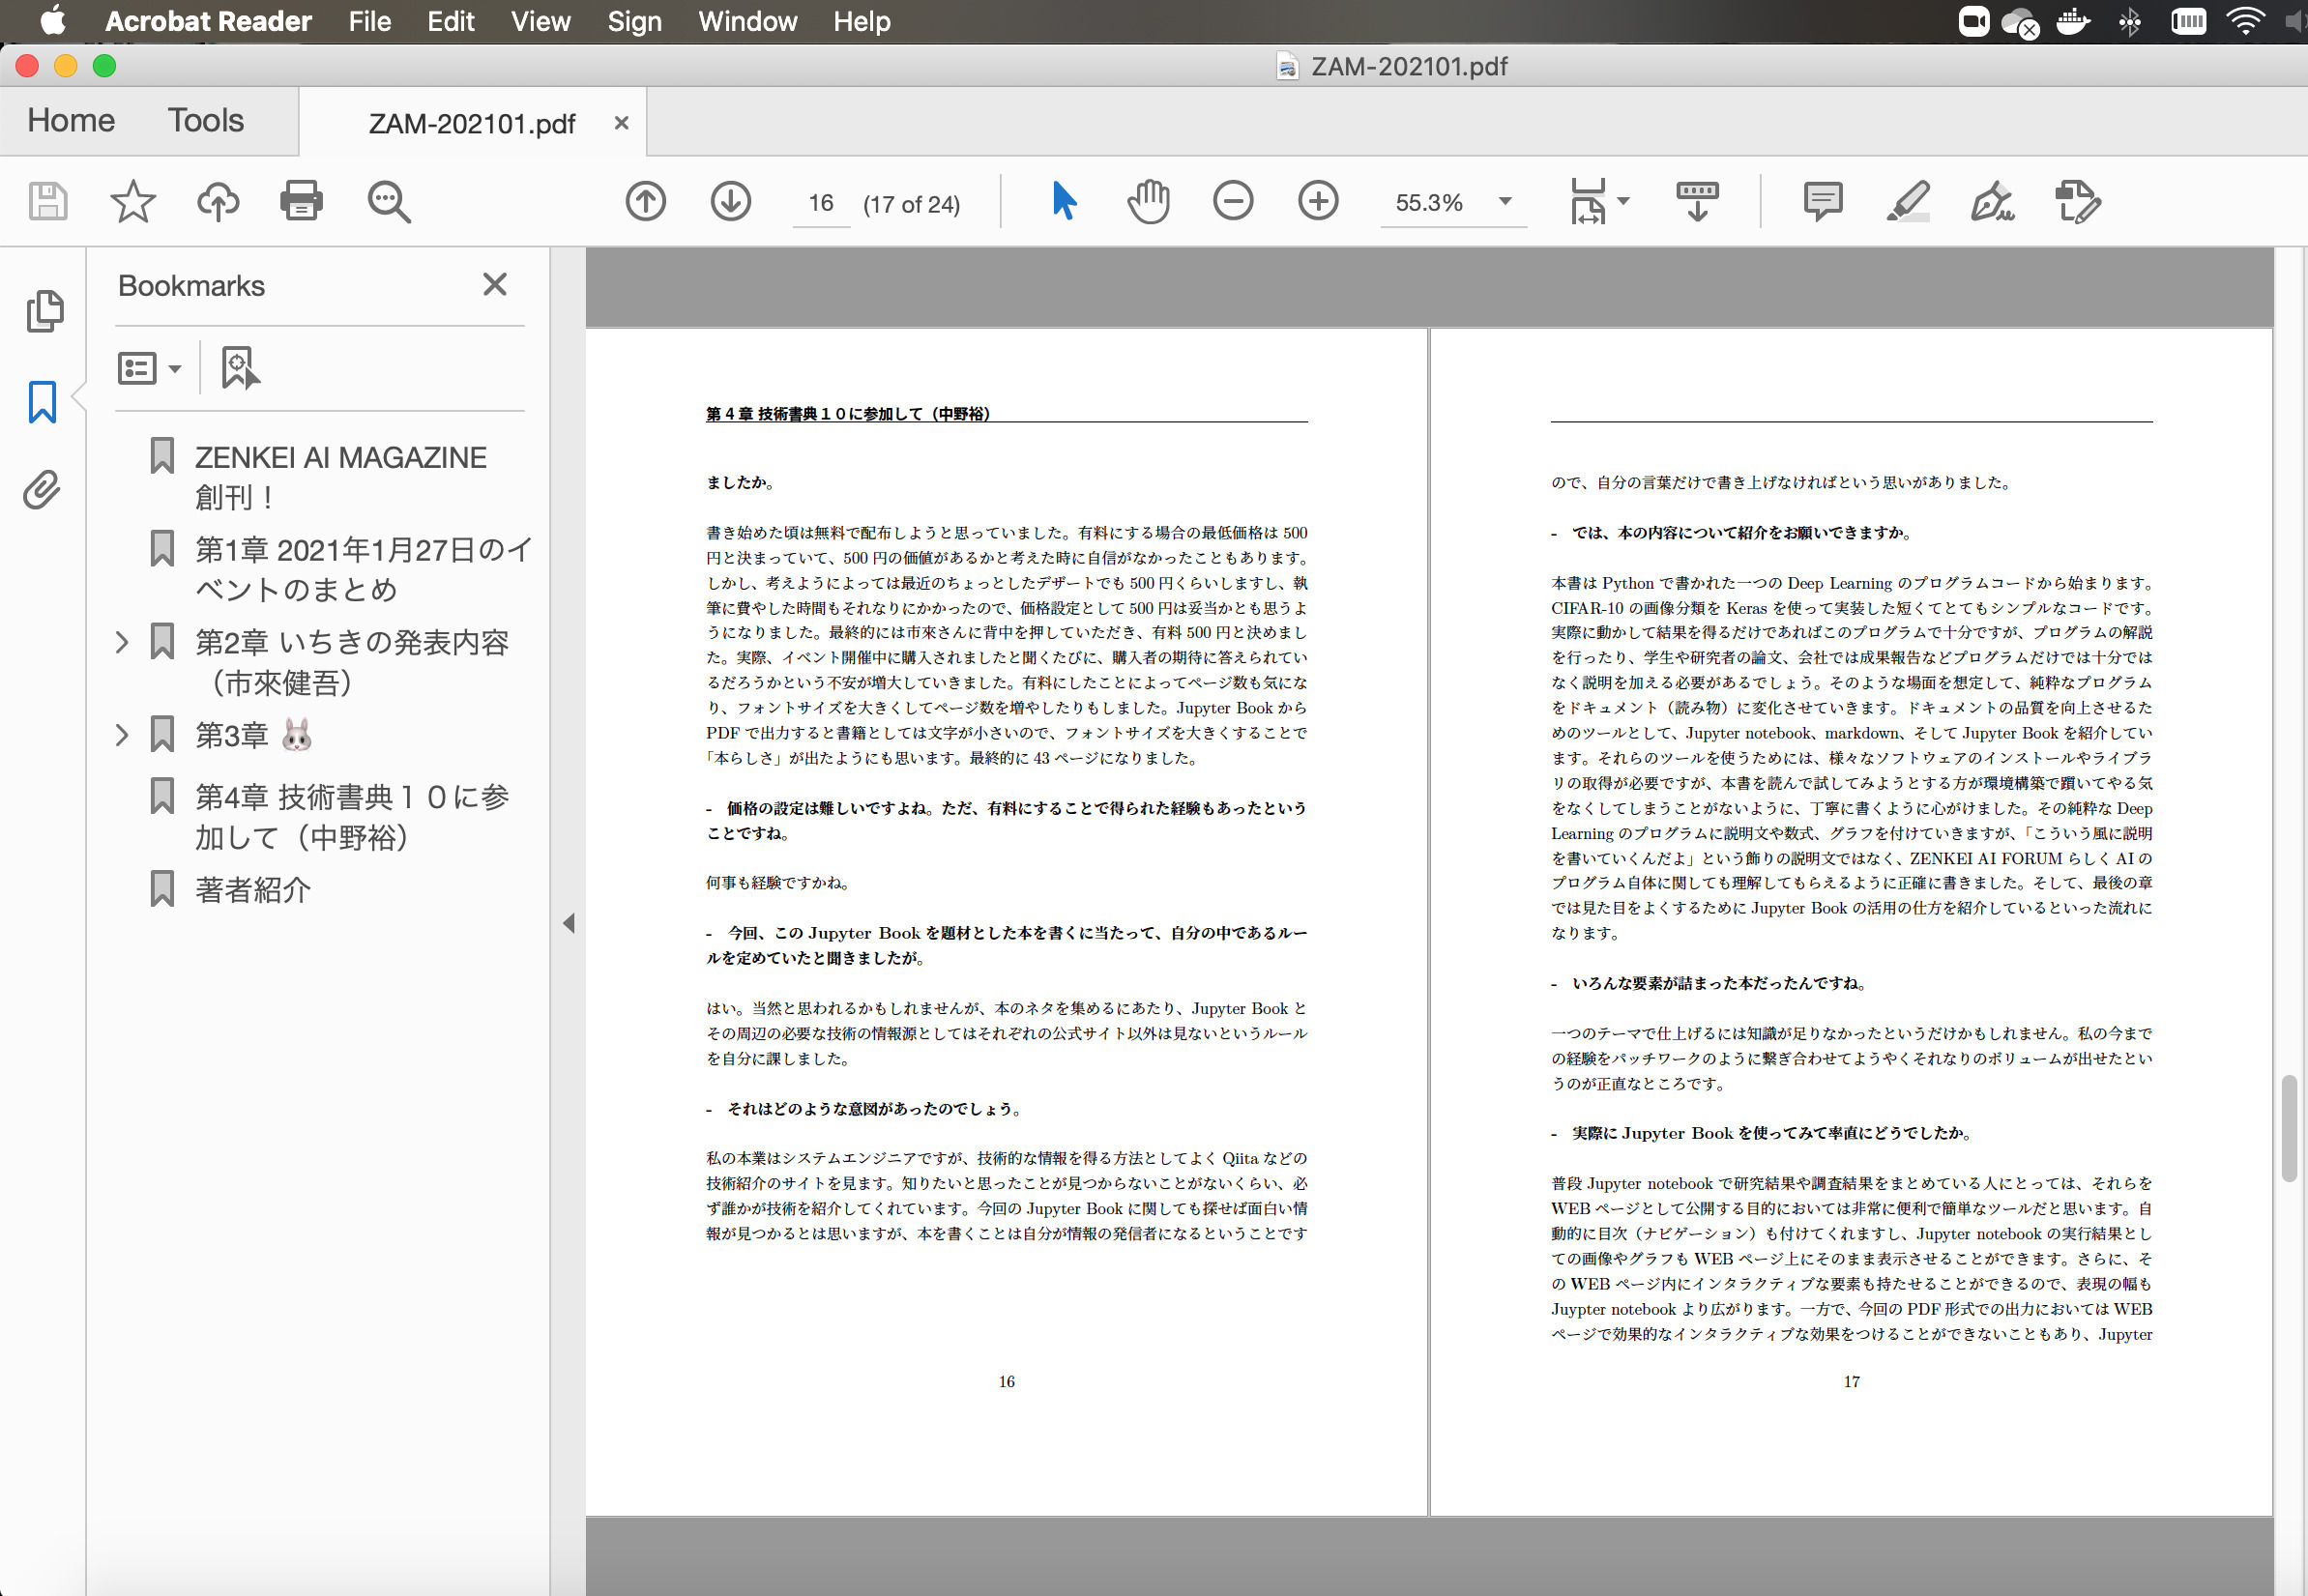
\includegraphics[height=0.18\textheight]
      {images/ZAM202101-pdf-03.jpg}
  };  
\end{tikzpicture}
\begin{tikzpicture}[remember picture, overlay]
  \node[xshift=7.4cm,yshift=-1.5cm] at (current page.center){
    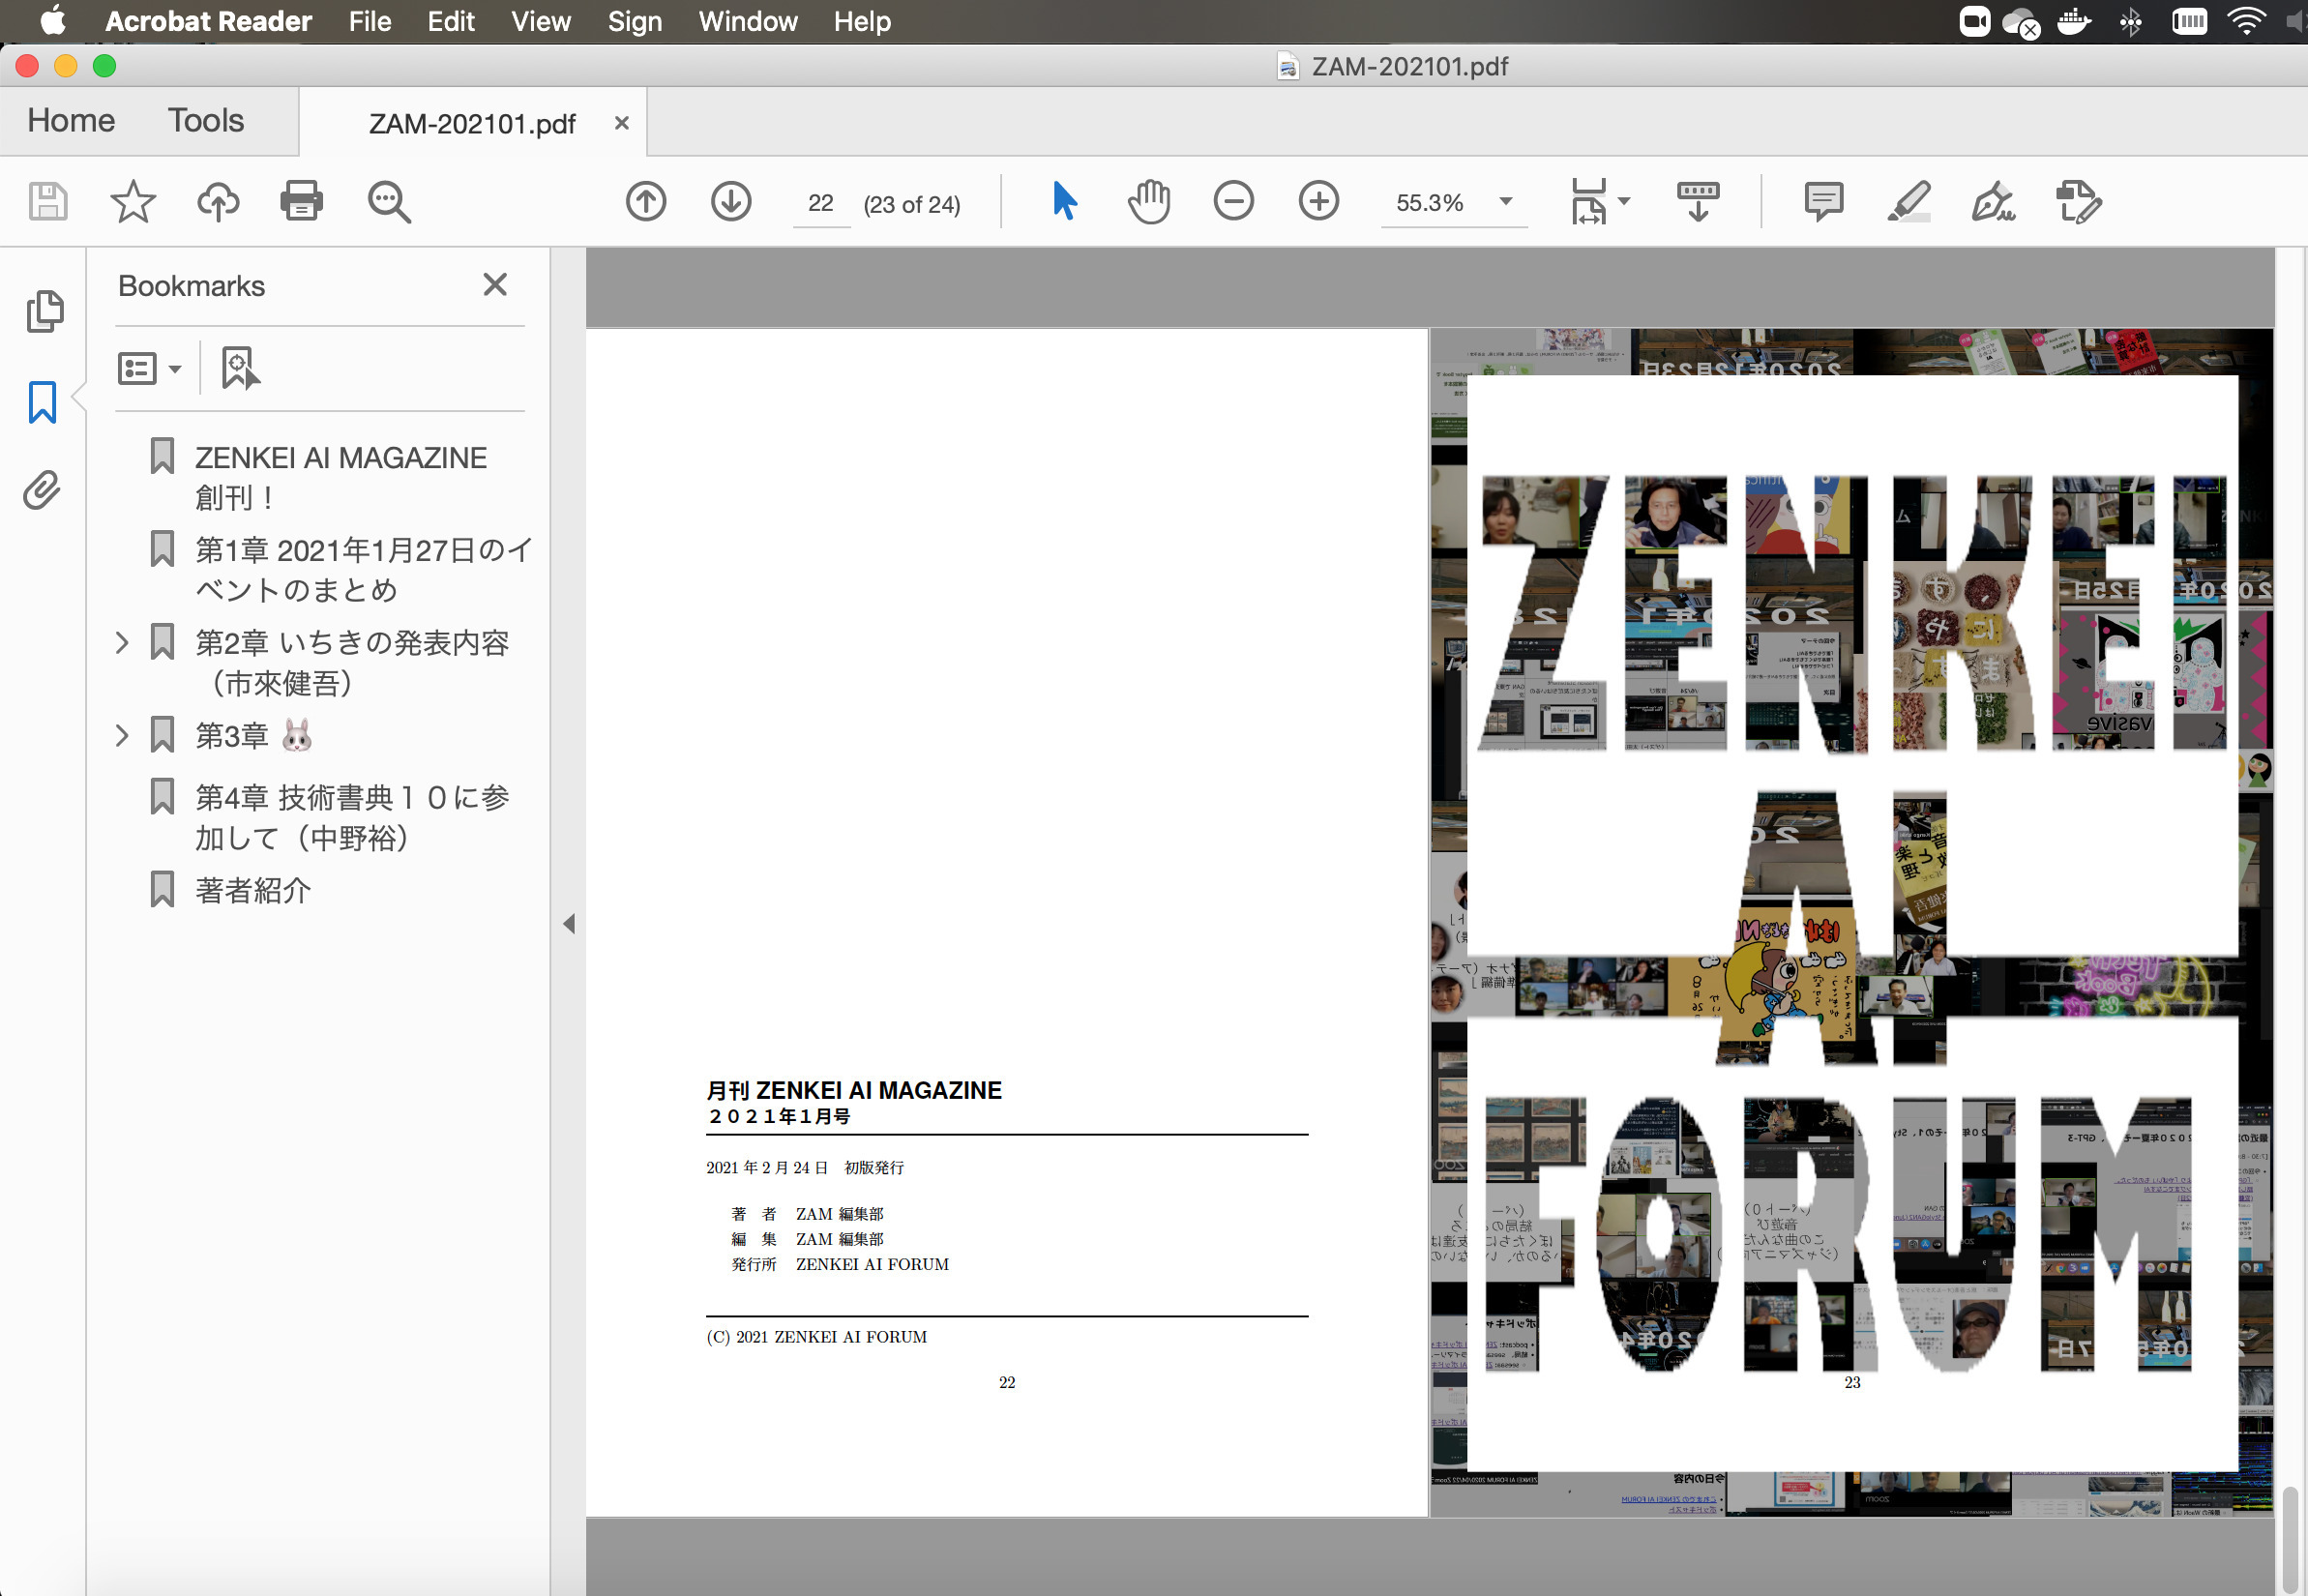
\includegraphics[height=0.18\textheight]
      {images/ZAM202101-pdf-04.jpg}
  };  
\end{tikzpicture}

\vspace{0.175\textheight}

\begin{center}
  PDF 版『月刊 ZAM』創刊号のスクショ
\end{center}

\hrule

\begin{multicols}{2}

\section{表紙について}
雑誌といえば、表紙ですね(もちろん中身も大事ですが)。
雑誌は定期刊行物であり、デザインはその雑誌の個性を反映する重要なファクターであり、
表紙はその中でも最も重要なデザイン要素になります。
わたしの見た感じだと、表紙のデザインに対して、大きく2通りの考え方があるようです。
\begin{itemize}
\item どの号も基本的に同じデザイン
\item 各号ごとに全く異なるデザイン
\end{itemize}
前者が majority かな?背景写真くらいが入れ替わったくらいで、
雑誌のタイトルが大きく入り、そのデザインはずっと同じデザインのタイプ。
後者は、各号おそらくデザイナーが変わって、内容に応じたデザインを採用するタイプ。
各号の特集に応じてガラッと異なった表紙デザインになっている
『WIRED』(日本語版)が印象に強くあります。
今回 ZAM を創刊するにあたり、わたしの念頭にはこんなイメージがありました。
実際に ZAF は話題が固定されていないし、
多様性 (diversity) こそが ZAF の目指すものだ、という思いもあります。

\end{multicols}

\hrule

\vspace{6cm}

\begin{tikzpicture}[remember picture, overlay]
  \node[xshift=0.0cm,yshift=1.0cm] at (current page.center){
    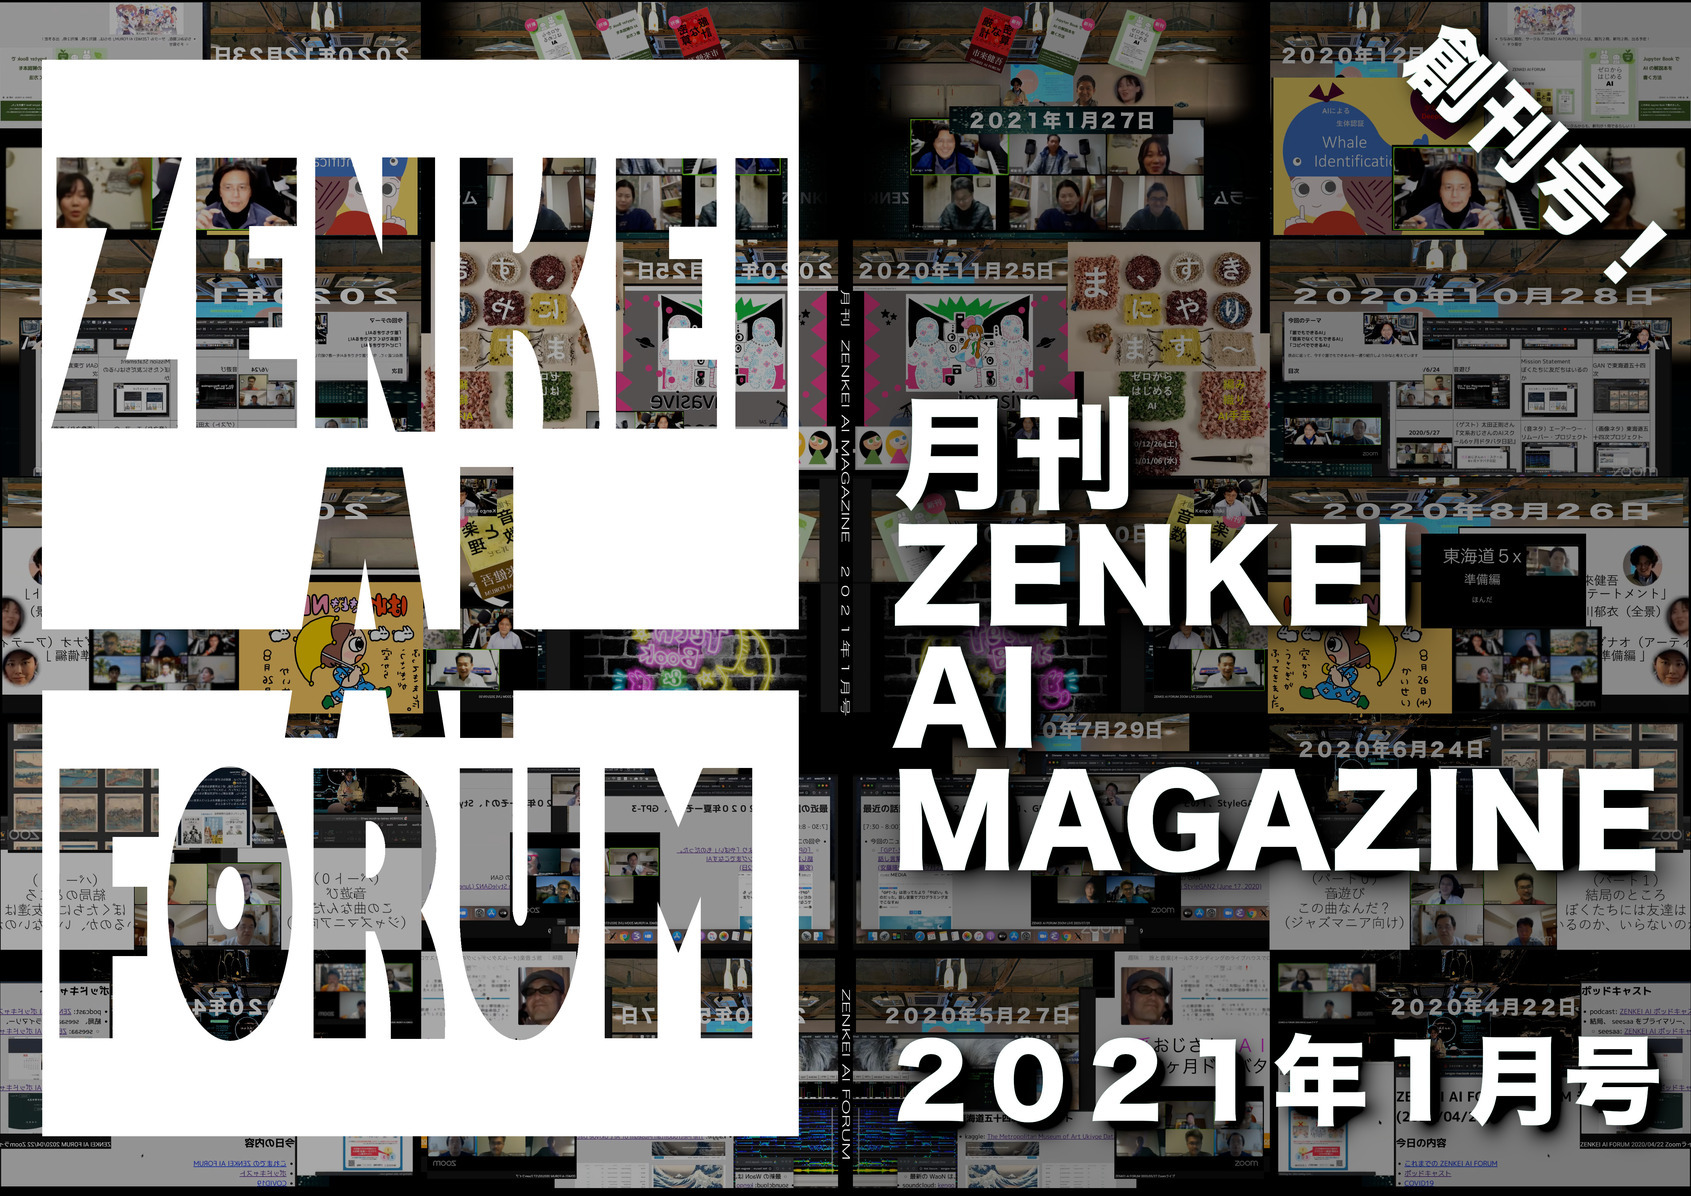
\includegraphics[width=1.3\textwidth]
      {images/ZAM202101-cover14.jpg}
  };  
\end{tikzpicture}

\vspace{8cm}

\hrule

\begin{multicols}{2}

そういうことで、創刊号の表紙デザインはわたしが担当しました。
コラージュって、なんか好きなんですよね。
レコード(CD)のジャケットとかでも
Pat Metheny Group は印象的でした。
素人デザインですが、これまでの ZAF を振り返りつつ、
いい感じにできたと自画自賛しています。

今後、各号の表紙デザインはそのときどき、才能あふれる ZAF メンバーなどに声をかけて、
見た目も楽しい雑誌になったらいいな、と思っています。

 % 全隠すページ

\end{multicols}

 % 全角スペース

\vspace{6cm}

\begin{multicols}{2}
\color{white}

\noindent
 % 全角スペース

 % 全角スペース

 % 全角スペース

 % 全角スペース
\begin{tikzpicture}[remember picture,overlay]
\node[xshift=3.7cm,yshift=-3.80cm,xscale=-1,color=white]
  at (current page.north){%
    ました。実際に ZAF は話題が固定されていな};
\node[xshift=3.7cm,yshift=-4.40cm,xscale=-1,color=white]
  at (current page.north){%
    いし、多様性 (diversity) こそが ZAF の目指す};
\node[xshift=-2.6cm,yshift=-3.80cm,xscale=-1,color=white]
  at (current page.north){%
    ものだ、という思いもあります。};
\node[xshift=-0.4cm,yshift=-4.40cm,color=white]
  at (current page.north){%
    ね};
\end{tikzpicture}

\end{multicols}

\hrule

\vspace{6cm}

\thispagestyle{fancy}
\lhead{\thepage}
\chead{}
\rhead{\leftmark}
\lfoot{}
\cfoot{}
\rfoot{}
\AddToShipoutPictureBG*{%
  \AtPageLowerLeft{%
    % Your background image here
    \includegraphics[width=\paperwidth,height=\paperheight]%
      {images/ZAM202102-p28-bg.jpg}
  }%
}%
\begin{tikzpicture}[remember picture, overlay]
  %\node[xshift=0.0cm,yshift=1.5cm] at (current page.center){
  \node[xshift=0.0cm,yshift=1.0cm] at (current page.center){
    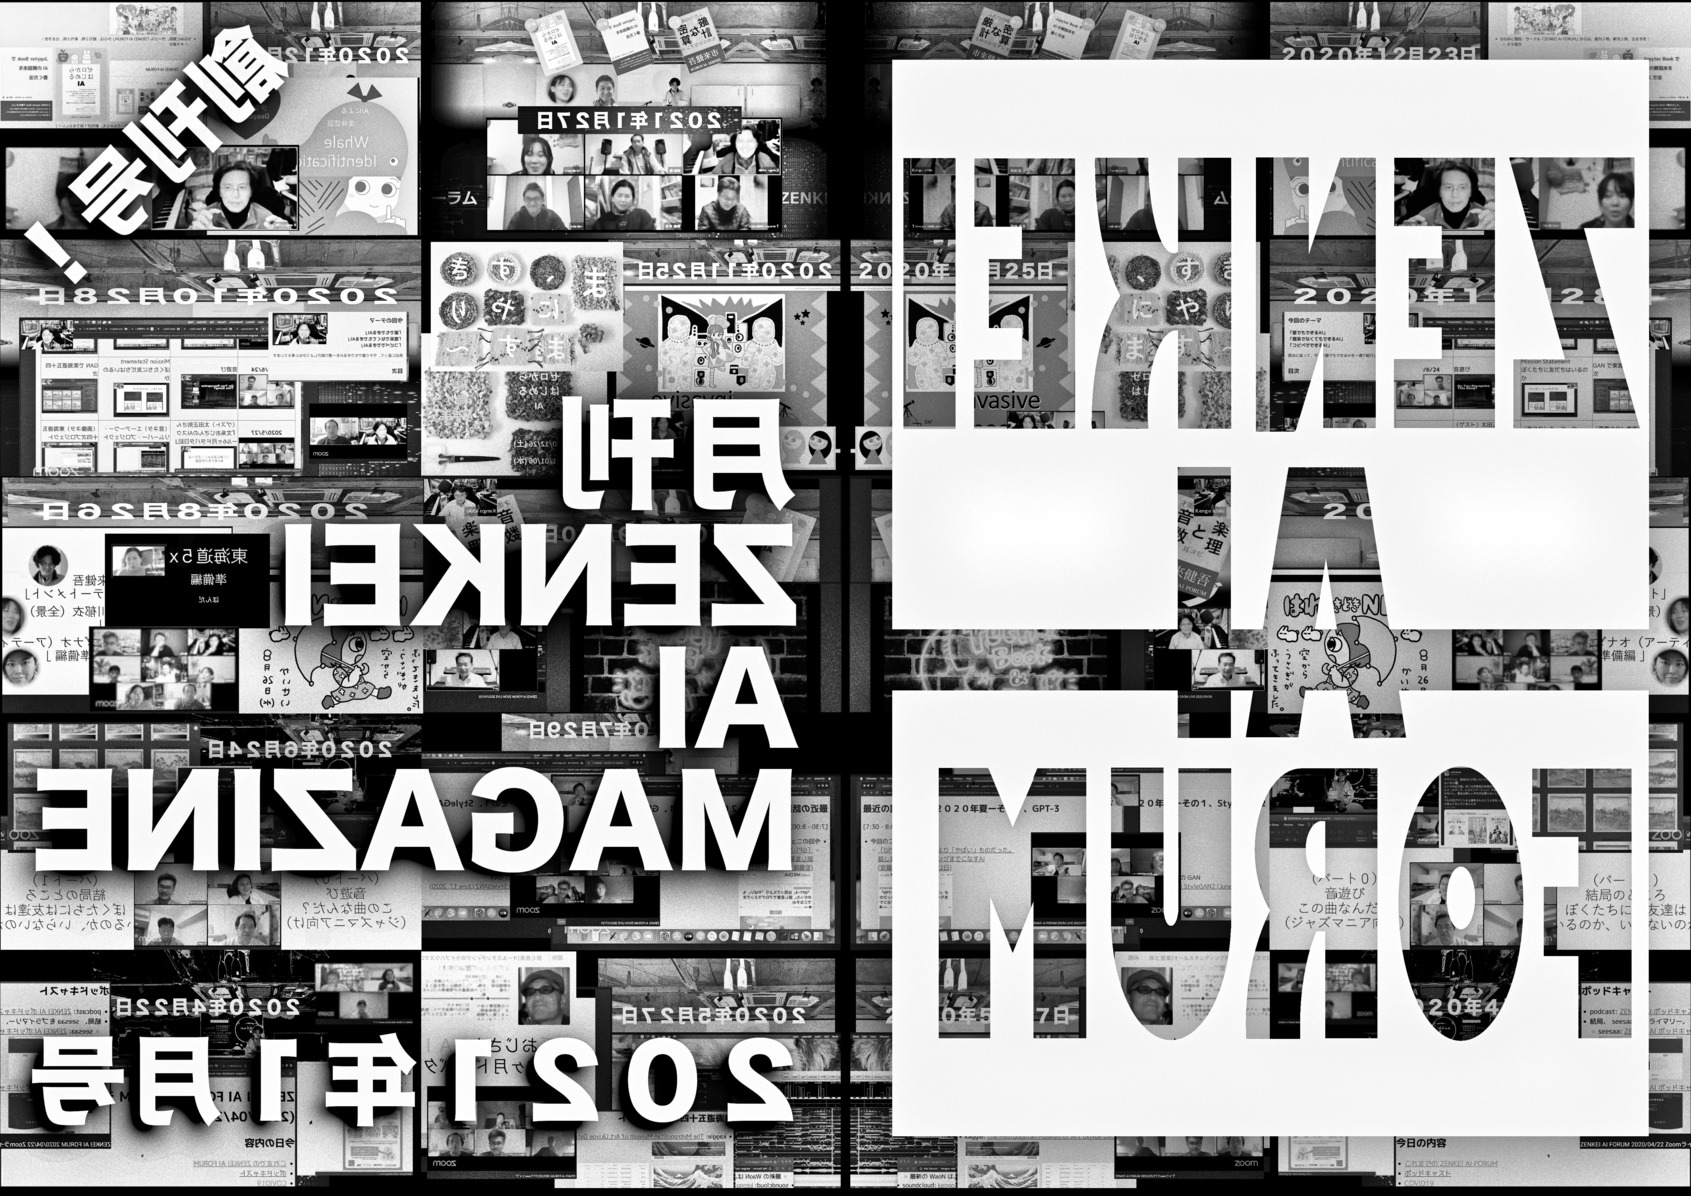
\includegraphics[width=1.3\textwidth]
      {images/ZAM202101-cover23.jpg}
  };  
\end{tikzpicture}

\vspace{8cm}

\hrule

\begin{multicols}{2}
\color{white}

 % 全角スペース

 % 全角スペース

 % 全角スペース

 % 全角スペース

 % 全角スペース

 % 全角スペース

 % 全角スペース

 % 全角スペース

 % 全角スペース

 % 全角スペース

 % 全角スペース

 % 全角スペース
\end{multicols}
\begin{tikzpicture}[remember picture,overlay]
\node[xshift=3.6cm,yshift=6.00cm,xscale=-1,color=white]
  at (current page.south){%
    そういうことで、創刊号の表紙デザインはわ};
\node[xshift=3.7cm,yshift=5.50cm,xscale=-1,color=white]
  at (current page.south){%
    たしが担当しました。コラージュって、なんか};
\node[xshift=3.7cm,yshift=5.00cm,xscale=-1,color=white]
  at (current page.south){%
    好きなんですよね。レコード(CD)のジャケッ};
\node[xshift=3.7cm,yshift=4.50cm,xscale=-1,color=lightgray]
  at (current page.south){%
    トとかでも Pat Metheny Group は印象的でし};
\node[xshift=3.7cm,yshift=4.00cm,xscale=-1,color=gray]
  at (current page.south){%
    た。素人デザインですが、これまでの ZAF を};
\node[xshift=3.7cm,yshift=3.50cm,xscale=-1,color=darkgray]
  at (current page.south){%
    振り返りつつ、いい感じにできたと自画自賛し};
\node[xshift=-1.0cm,yshift=6.00cm,xscale=-1,color=white]
  at (current page.south){%
    ています。};
\node[xshift=-3.5cm,yshift=5.50cm,xscale=-1,color=white]
  at (current page.south){%
    今後、各号の表紙デザインはそのときどき、};
\node[xshift=-3.7cm,yshift=5.00cm,xscale=-1,color=white]
  at (current page.south){%
    才能あふれる ZAF メンバーなどに声をかけて、};
\node[xshift=-3.7cm,yshift=4.50cm,xscale=-1,color=lightgray]
  at (current page.south){%
    見た目も楽しい雑誌になったらいいな、と思っ};
\node[xshift=-1.0cm,yshift=4.00cm,xscale=-1,color=gray]
  at (current page.south){%
    ています。};
\end{tikzpicture}
% 5
\begin{tikzpicture}[remember picture, overlay]
  \begin{scope}[thick,rounded corners=8pt, color=red,
      line width=8pt,
      %xscale=-1.3, yscale=1.3, xshift=-12.25cm, yshift=-1.2cm]
      xscale=-1.3, yscale=1.3, xshift=-12.2cm, yshift=-1.2cm]
  \draw (0, 2) -- (5, 2) -- (4, 0) [sharp corners] -- (5.5, 0)
    [rounded corners=8pt] -- (6.5, 2) [sharp corners] -- (7.5, 0)
    -- (8.5, 0);
  \draw (3.5, 0.8) -- (7.5, 0.8)
    -- (8.2, 2) -- (9.2, 0) -- (10.2, 2) -- (10.2, 0) -- (14, 0);
  \end{scope}
\end{tikzpicture}


\newpage
\thispagestyle{fancy}
\lhead{\rightmark}
\rhead{\thepage}
\color{white}

\begin{multicols}{2}

\AddToShipoutPictureBG*{%
  \AtPageLowerLeft{%
    % Your background image here
    \includegraphics[width=\paperwidth,height=\paperheight]%
      {images/ZAM202102-p29-bg.jpg}
  }%
}%
\section{終わって……ない}
という報告を持って、
めでたく2月の(わたし、市來健吾の独演会になってしまった)
ZENKEI AI FORUM は無事終了!

と思ったのですが、
実は ZAF の終わりは ZAM の始まり、
という仕組みを(自分で)作ったんですね。

そういうことで、この瞬間から ZAM 第2号の編集作業が始まります。
(と、今ここに必死にこの ZAM 第2号を仕上げるために書いています。)

ちなみに本号の表紙デザインは、
いつも ZAF や『技術書典』イベントでたくさんイラストを描いてくれている
furukawa さんにお願いしました。

\end{multicols}

% 5 - triple thickening
\begin{tikzpicture}[remember picture, overlay]
  \begin{scope}[thick,rounded corners=8pt, color=white,
      xscale=1.3, yscale=1.3, xshift=-1.75cm, yshift=-6.5cm]
  \draw (0, 2) -- (5, 2) -- (4, 0) -- (5.5, 0);
  \draw (5.5, 0) -- (6.5, 2) -- (7.5, 0);
  \draw (7.5, 0) -- (8.5, 0);
  \draw (3.5, 0.8) -- (7.5, 0.8)
    -- (8.2, 2) -- (9.2, 0) -- (10.2, 2) -- (10.2, 0) -- (14, 0);
  \end{scope}
  \begin{scope}[thick,rounded corners=8pt,
      line width=4pt,
      xscale=1.3, yscale=1.3, xshift=-1.75cm, yshift=-9.5cm]
  \draw (0, 2) -- (5, 2) -- (4, 0) [sharp corners] -- (5.5, 0)
    [rounded corners=8pt] -- (6.5, 2) [sharp corners] -- (7.5, 0)
    -- (8.5, 0);
  \draw (3.5, 0.8) -- (7.5, 0.8)
    -- (8.2, 2) -- (9.2, 0) -- (10.2, 2) -- (10.2, 0) -- (14, 0);
  \end{scope}
  \begin{scope}[thick,rounded corners=8pt,
      line width=8pt, color=red,
      xscale=1.3, yscale=1.3, xshift=-1.75cm, yshift=-12.5cm]
  \draw (0, 2) -- (5, 2) -- (4, 0) [sharp corners] -- (5.5, 0)
    [rounded corners=8pt] -- (6.5, 2) [sharp corners] -- (7.5, 0)
    -- (8.5, 0);
  \draw (3.5, 0.8) -- (7.5, 0.8)
    -- (8.2, 2) -- (9.2, 0) -- (10.2, 2) -- (10.2, 0) -- (14, 0);
  \end{scope}
\end{tikzpicture}

\pagecolor{white}
\color{black}

\titleformat{\chapter}[block]
{\gtfamily\bfseries \Huge} % style
{\bfseries \huge 第 \thechapter 章\\} % label
{0pt} % spacing
{} % in front of the title
[]

\chapter*{編集後記}
\addcontentsline{toc}{chapter}{編集後記}
\AddToShipoutPictureBG*{%
  \AtPageLowerLeft{%
    % Your background image here
    \includegraphics[width=\paperwidth,height=\paperheight]%
      {images/ZAM202102-p31-bg.jpg}
  }%
}%
\begin{tikzpicture}[
  remember picture, overlay]
\node[yshift=-8em,yscale=1.2,xslant=0.25,color=Gray] (text)
  at (current page.north){%
  \sffamily \large
  【月刊 ZENKEI AI MAGAZINE 2021年2月号】};
\node[anchor=south,yscale=0.8,color=BlueViolet]
  at (text.north){%
  \pgfornament[width=\textwidth]{71}};
\end{tikzpicture}

{\mcfamily\rmfamily
本文にもたくさん(愚痴のように)書きましたが、
なんとか『月刊 ZENKEI AI MAGAZIN』の2冊目、
2021年2月号が仕上がりました。

ZENKEI AI FORUM の文字化、ということで、
2月の登壇者がわたし一人という事態に(ZAM 2号目で)なってしまい、
結局これってこれまでの単行本書いてた『技術書典』じゃないか、
と思ったりもしました。
しかし書き終わった今、これも1つの通過儀礼だと思っています。

これからも、がんばります。

\begin{flushright}
  (市來健吾)
\end{flushright}
}

% rainbow
\begin{tikzpicture}[remember picture, overlay,
    xscale=1.5, yscale=1.5, xshift=-2.5cm, yshift=-7cm]
  \begin{scope}[thick, rounded corners=8pt,color=red]
  \draw (0, 2) -- (5, 2) -- (4, 0) -- (5.5, 0);
  \draw (5.5, 0) -- (6.5, 2) -- (7.5, 0);
  \draw (7.5, 0) -- (8.5, 0);
  \draw (3.5, 0.8) -- (7.5, 0.8)
    -- (8.2, 2) -- (9.2, 0) -- (10.2, 2) -- (10.2, 0) -- (14, 0);
  \end{scope}

  \begin{scope}[thick, rounded corners=8pt,color=orange,
      xshift=0.04cm,yshift=-0.1cm]
  \draw (0, 2) -- (5, 2) -- (4, 0) -- (5.5, 0);
  \draw (5.5, 0) -- (6.5, 2) -- (7.5, 0);
  \draw (7.5, 0) -- (8.5, 0);
  \draw (3.5, 0.8) -- (7.5, 0.8)
    -- (8.2, 2) -- (9.2, 0) -- (10.2, 2) -- (10.2, 0) -- (14, 0);
  \end{scope}

  \begin{scope}[thick, rounded corners=8pt,color=yellow,
      xshift=0.08cm,yshift=-0.2cm]
  \draw (0, 2) -- (5, 2) -- (4, 0) -- (5.5, 0);
  \draw (5.5, 0) -- (6.5, 2) -- (7.5, 0);
  \draw (7.5, 0) -- (8.5, 0);
  \draw (3.5, 0.8) -- (7.5, 0.8)
    -- (8.2, 2) -- (9.2, 0) -- (10.2, 2) -- (10.2, 0) -- (14, 0);
  \end{scope}

  \begin{scope}[thick, rounded corners=8pt,color=green,
      xshift=0.12cm,yshift=-0.3cm]
  \draw (0, 2) -- (5, 2) -- (4, 0) -- (5.5, 0);
  \draw (5.5, 0) -- (6.5, 2) -- (7.5, 0);
  \draw (7.5, 0) -- (8.5, 0);
  \draw (3.5, 0.8) -- (7.5, 0.8)
    -- (8.2, 2) -- (9.2, 0) -- (10.2, 2) -- (10.2, 0) -- (14, 0);
  \end{scope}

  \begin{scope}[thick, rounded corners=8pt,color=blue,
      xshift=0.16cm,yshift=-0.4cm]
  \draw (0, 2) -- (5, 2) -- (4, 0) -- (5.5, 0);
  \draw (5.5, 0) -- (6.5, 2) -- (7.5, 0);
  \draw (7.5, 0) -- (8.5, 0);
  \draw (3.5, 0.8) -- (7.5, 0.8)
    -- (8.2, 2) -- (9.2, 0) -- (10.2, 2) -- (10.2, 0) -- (14, 0);
  \end{scope}

  \begin{scope}[thick, rounded corners=8pt,color=BlueViolet,
      xshift=0.2cm,yshift=-0.5cm]
  \draw (0, 2) -- (5, 2) -- (4, 0) -- (5.5, 0);
  \draw (5.5, 0) -- (6.5, 2) -- (7.5, 0);
  \draw (7.5, 0) -- (8.5, 0);
  \draw (3.5, 0.8) -- (7.5, 0.8)
    -- (8.2, 2) -- (9.2, 0) -- (10.2, 2) -- (10.2, 0) -- (14, 0);
  \end{scope}

  \begin{scope}[thick, rounded corners=8pt,color=violet,
      xshift=0.24cm,yshift=-0.6cm]
  \draw (0, 2) -- (5, 2) -- (4, 0) -- (5.5, 0);
  \draw (5.5, 0) -- (6.5, 2) -- (7.5, 0);
  \draw (7.5, 0) -- (8.5, 0);
  \draw (3.5, 0.8) -- (7.5, 0.8)
    -- (8.2, 2) -- (9.2, 0) -- (10.2, 2) -- (10.2, 0) -- (14, 0);
  \end{scope}

\end{tikzpicture}

\newpage

\AddToShipoutPictureBG*{%
  \AtPageLowerLeft{%
    % Your background image here
    \includegraphics[width=\paperwidth,height=\paperheight]%
      {images/ZAM202102-p31-bg.jpg}
  }%
}%

 %全角スペース

\vspace{3cm}

\begin{center}
\begin{tikzpicture}[every node/.style={inner sep=0pt}]   
  \node[text width=8cm,align=center](Text){%
  {\Large {\gtfamily\bfseries 謝辞に代えて}}\\
  \vspace{24pt}
  ZENKEI AI FORUM のみなさま\\
  いつもありがとうございます。\\
  \bigskip
  本号は \LaTeX で版組みしました。\\
  奥村晴彦著『{\bfseries \LaTeXe 美文書作成入門}』の\\
  \texttt{jsbook} スタイルを使用しました。\\
  \bigskip
  今回はじめて使った全くの初心者ですが\\
  \texttt{tikz} で図や写真の配置など行いました。\\
  装飾は \href{http://altermundus.fr/includes/pgfornament.php}{\texttt{pgfornament}} パッケージを使用しました。\\
  \vspace{24pt}
  数多くの人に支えられてます。\\
  ありがとうございます。
} ;
%\color{teal}
%\color{olive}
\color{BlueViolet}
%\color{RedViolet}
\node[shift={(-1cm,1cm)},anchor=north west](CNW)  at (Text.north west)
               {\pgfornament[width=2cm]{61}};
\node[shift={(1cm,1cm)},anchor=north east](CNE)   at (Text.north east)
               {\pgfornament[width=2cm,symmetry=v]{61}}; 
\node[shift={(-1cm,-1cm)},anchor=south west](CSW) at (Text.south west)
               {\pgfornament[width=2cm,symmetry=h]{61}}; 
\node[shift={(1cm,-1cm)},anchor=south east](CSE)  at (Text.south east)   
               {\pgfornament[width=2cm,symmetry=c]{61}};  
\pgfornamenthline{CNW}{CNE}{north}{87}
\pgfornamenthline{CSW}{CSE}{south}{87}
\pgfornamentvline{CNW}{CSW}{west}{87}
\pgfornamentvline{CNE}{CSE}{east}{87} 
\color{black}
\end{tikzpicture}
\end{center}


 % 全角スペース
% 奥付ページ
% cf. https://yamaimo.hatenablog.jp/entry/2019/09/23/200000
\clearpage
%\thispagestyle{empty}
\thispagestyle{plain}
\makeatletter
    \ifodd\c@page
        %\hbox{}\newpage\thispagestyle{empty}
        \hbox{}\newpage\thispagestyle{plain}
    \fi
\makeatother

\AddToShipoutPictureBG*{%
  \AtPageLowerLeft{%
    % Your background image here
    \includegraphics[width=\paperwidth,height=\paperheight]%
      {images/ZAM202102-cover-2-v2-masked.jpg}
  }%
}%
\vspace*{\fill}

% 奥付
\begin{flushleft}
  \begin{tabular*}{\textwidth}{@{}l@{\extracolsep{\fill}}}
    {\LARGE \gtfamily\bfseries 月刊 ZENKEI AI MAGAZINE}\\
    {\Large \gtfamily\bfseries 2021年2月号}\\
    \bhline{1pt}
    \begin{tabular}{@{}r@{年\kern.5zw}r@{月\kern.5zw}r@{日\kern1.5zw}ll}
      2021 & 4 & 7 & 初版発行 & (オンライン)\\
      2021 & 4 & 15 & 改訂版発行 & (第1刷)\\
    \end{tabular} \\
    \\
    \begin{tabular}{@{}l@{\kern.5zw\textbf{:}\kern1zw}l}
      編 集 & ZAM 編集部\\
      発行所 & ZENKEI AI FORUM\\
      連絡先 & \url{https://forum.ai.zenkei.com/} \\
      表 紙 & furukawa \\
      印刷所 & ちょ古っ都製本工房 \url{https://www.chokotto.jp/} \\
    \end{tabular} \\
    \bhline{1pt}
    \texttt{%
      \textcopyright\quad
      ZENKEI AI FORUM\quad
      2021,\quad
      Printed in Japan
    }
  \end{tabular*}
\end{flushleft}

\end{document}
